\documentclass[a4paper,11pt,oneside]{book}
\title{\textbf{Applicazioni di una nuova teoria perturbativa multireference allo
studio dello stato fondamentale e degli stati eccitati di molecole di medie
dimensioni}}
\author{Stefano Borini}
\usepackage[italian]{babel}
\usepackage[latin1]{inputenc}
\usepackage[T1]{fontenc}
\usepackage{amssymb}
\usepackage{graphics}
\usepackage{amsmath}
\usepackage{geometry}
\usepackage{amssymb}
\usepackage{graphicx}
\usepackage{threeparttable}
\usepackage{wrapfig}
%\usepackage{floatflt}
%\usepackage{fancyhdr}
%\usepackage{acsarticle}
\usepackage[hang, bf]{caption}
%\usepackage{xymtex}
%\usepackage{chemist}

\geometry{a4paper,tmargin=28mm,bmargin=42mm,lmargin=4cm,rmargin=4cm}
%\geometry{a4paper,tmargin=50mm,bmargin=20mm,lmargin=4cm,rmargin=4cm}
%\addtolength\evensidemargin{7mm}
\headsep=10mm
\makeatletter
\@addtoreset{equation}{section}
\@addtoreset{table}{section}
\@addtoreset{figure}{section}
\makeatother
\renewcommand{\theequation}{\arabic{chapter}.\arabic{section}.\arabic{equation}}
\renewcommand{\thetable}{\arabic{chapter}.\arabic{section}.\arabic{table}}
\renewcommand{\thefigure}{\arabic{chapter}.\arabic{section}.\arabic{figure}}

% sommatorie 
\newcommand{\sumoneinf}[1]{\sum_{#1 = 1}^{+\infty}}
\newcommand{\sumonen}[1]{\sum_{#1 = 1}^{n}}
\newcommand{\sumonenprime}[1]{\sumonen{#1} \! {}^{\prime}}
\newcommand{\sumalpha}{\sum_{\alpha = 1}^{N}}
\newcommand{\sumidx}[1]{\sum_{#1}}
\newcommand{\sumidxprm}[1]{\sum_{#1} \! {}^{\prime}}

% alcune macro utili
\newcommand{\beq}{\begin{equation}}
\newcommand{\eeq}{\end{equation}}
\newcommand{\beqa}{\begin{eqnarray}}
\newcommand{\eeqa}{\end{eqnarray}}
\newcommand{\beqas}{\begin{eqnarray*}}
\newcommand{\eeqas}{\end{eqnarray*}}

% hamiltoniani ed altri operatori
\newcommand{\ham}{\hat{\mathcal{H}}}
\newcommand{\hamel}{\hat{\mathcal{H}}_{el}}
\newcommand{\hamtot}{\hat{\mathcal{H}}_{tot}}
\newcommand{\fock}{\hat{\mathcal{F}}}

% energia totale
\newcommand{\etot}{E_{tot}}

% psi (varie)
\newcommand{\psia}{\psi_a}
\newcommand{\psii}{\psi_i}
\newcommand{\psij}{\psi_j}
\newcommand{\psik}{\psi_k}
\newcommand{\psil}{\psi_l}
\newcommand{\psin}{\psi_n}
\newcommand{\psim}{\psi_m}
\newcommand{\psitilde}{\tilde{\psi}}
\newcommand{\psitot}{\psi_{tot}}
\newcommand{\psiixq}{\psii \left(x,\! Q\right)}
\newcommand{\psiixqp}{\psii \left(x;\! Q\right)}
\newcommand{\psitotxq}{\psitot \left(x,\! Q\right)}
\newcommand{\psitotxqp}{\psitot \left(x;\! Q\right)}

% costanti frequenti
\newcommand{\half}{\frac{1}{2}}
\newcommand{\hfrac}{\frac{\hbar^2}{2}}
\newcommand{\hfracm}{\frac{\hbar^2}{2 m} }

% derivate
\newcommand{\dpart}[1]{\frac{\partial}{\partial #1}}
\newcommand{\ddpart}[1]{\frac{\partial^2}{\partial #1^2}}
\newcommand{\dpartfrac}[2]{\frac{\partial #1}{\partial #2}}
\newcommand{\ddpartfrac}[2]{\frac{\partial^2 #1}{\partial #2^2}}
\newcommand{\nablavect}[1]{\overrightarrow{\nabla} \!\! _#1}
\newcommand{\nablaquad}[1]{\nabla^2 \! \! \! _#1}

% braket

\newcommand{\bra}[1]{\left\langle #1 \right|}
\newcommand{\ket}[1]{\left| #1 \right\rangle}
\newcommand{\vacuum}{\left| \mbox{vac} \right\rangle}
\newcommand{\braket}[3]{\left\langle #1 \left| #2 \right| #3 \right\rangle}
\newcommand{\integral}[2]{\left\langle #1 \left.\right| #2 \right\rangle}
\newcommand{\interact}[2]{\left\langle #1 \left| \right| #2 \right\rangle}

% altri

\newcommand{\adiab}{\hat{\Lambda}_{ki}}
\newcommand{\abs}[1]{\left| #1 \right|}

% orbitali e analoghi

\newcommand{\pistar}{\pi^{*}}
\newcommand{\detsl}[1]{\left\Vert #1 \right\Vert}

% simboli ricorrenti
\newcommand{\constr}[1]{a_{#1}^{+}}
\newcommand{\destr}[1]{a_{#1}}
\newcommand{\proj}[1]{\hat{\mathcal{P}}_{#1}}
\newcommand{\perturb}{\hat{\mathcal{V}}}
\newcommand{\resolvent}{\frac{\mathcal{Q}_0}{a}}

% varie sigle
\newcommand{\dalton}{\texttt{DALTON}}



\raggedbottom
\begin{document}
\begin{titlepage}
\begin{center}
\begin{tabular}{c}
{\Large \textbf{UNIVERSIT\`A DEGLI STUDI DI FERRARA}} \\
{\Large \textit{Facolt\`a di Scienze Matematiche, Fisiche, Naturali}} \\
{\Large \textit{Corso di laurea in Chimica}} \\
\hline
\end{tabular}

\vspace{5cm}
{\textsc{\fontsize{17}{5mm}\selectfont \textbf{Applicazioni di una nuova\\teoria perturbativa multireference\\allo studio dello stato fondamentale\\e degli stati eccitati di molecole\\di medie dimensioni}}}

\vspace{45mm}

{ 
\begin{tabular}{l} \large \textbf{Relatore} \\ \large \textbf{Prof. Renzo Cimiraglia}
\end{tabular} \hfill {\ } } \\
\vspace{13mm}
{ \begin{tabular}{l} \large \textbf{Corelatore} \\ \large \textbf{Dott. Celestino Angeli}\end{tabular} } \hfill { \begin{tabular}{l} \large \textbf{Laureando} \\ \large \textbf{Stefano Borini} \end{tabular} }

\vspace{26mm}
\begin{tabular}{c}
\hline
{\large \textbf{ANNO ACCADEMICO 2001/2002}} \\
\hline
\end{tabular}

\end{center}
\end{titlepage}
%\newpage\thispagestyle{empty}\ \newpage
\pagenumbering{Roman}
\tableofcontents
\pagebreak
\thispagestyle{empty}

{ \Large \textbf{Ringraziamenti}}
\vspace{6mm}

Dopo una vita di impegno e di studio giungo, con questo lavoro di tesi,
ad una conclusione certamente ambita da tempo, ragionata, all'inseguimento
costante di quello che ho sempre desiderato ottenere prima di ogni cosa:
la conoscenza.

Tuttavia, la conoscenza \`e ben lungi dall'essere istintiva. \`E fatta di
buone basi, di sviluppi attenti e mirati, di interesse personale alimentato
da chi mi circondava e mi circonda tuttora, fornendomi la possibilit\`a di
accedere e comprendere le tante sfaccettature del mondo scientifico.

Per questa ragione, devo il raggiungimento di questo traguardo a chi mi ha
fornito gli strumenti e la cultura, ma soprattutto la fiducia.

Ringrazio quindi il Prof. Cimiraglia per aver tracciato un cammino di
apprendimento sicuro e razionale verso una disciplina complessa ma
affascinante, ricca di risvolti e collegamenti sempre pi\`u profondi
man mano che nuove conoscenze si aggiungevano a quelle gi\`a acquisite.

Ringrazio il Dott. Angeli, per la guida attenta e puntuale sugli sviluppi di
questo lavoro.

Ringrazio la Prof. Ruggiero, per avermi fornito gli strumenti adatti alla
comprensione di questa disciplina.

Ringrazio tutti gli insegnanti del mio percorso didattico, che grazie alla
loro passione e alle loro capacit\`a, sono stati in grado di infondere in me
sia le basi che il desiderio di apprendere e perfezionare sempre pi\`u le mie
conoscenze.

Ringrazio infine i miei genitori, che come insegnanti e come educatori mi
hanno fornito le capacit\`a e la forza di tenere duro nonostante le
difficolt\`a.

A tutti, grazie di cuore.



%\newpage\thispagestyle{empty}\ \newpage
\chapter{Introduzione}
\pagenumbering{arabic}

In questa prima parte verranno affrontate le teorie e le tecniche computazionali
utilizzate nell'elaborazione di questo lavoro di tesi. Di centrale importanza sar\`a
evidenziare le modalit\`a di risoluzione per l'approccio di studio \textit{ab initio}
su sistemi di modeste dimensioni, nonch\'e approfondire formalismi a livello
teorico per poter meglio apprezzare le successive fasi teoriche e applicative.

In primis ci occuperemo dell'approccio variazionale e perturbativo per ottenere
l'energia e la funzione d'onda adatta a descrivere uno stato elettronico.
Questi concetti
sono centrali sia dal punto di vista formale, permettendo un agevole metodo di
analisi attraverso l'algebra lineare, sia dal punto di vista numerico e
computazionale, perch\'e consentono di ottenere valori numerici da confrontare
con il dato sperimentale.

Successivamente, sar\`a presentata una concisa panoramica dei concetti base
della chimica teorica, per poi considerare in maniera pi\`u dettagliata la teoria
perturbativa NEV-PT, centrale nello sviluppo di questa tesi.

% DONE
\section{Principio variazionale}

Sia $\tilde{\Psi}$ una funzione d'onda arbitraria e si definisca il rapporto
\beq
\label{eqn:varia1}
\epsilon = \frac{\braket{\tilde{\Psi}}{\ham}{\tilde{\Psi}}}{\integral{\tilde{\Psi}}{\tilde{\Psi}}}
\eeq

Secondo il teorema variazionale, l'energia $E_0$, autovalore dello stato fondamentale $\Psi_0$ sull'hamiltoniano,
\`e un limite inferiore per $\epsilon$. In altri termini vale
\beq
\epsilon \ge E_0 \quad \forall \tilde{\Psi} \quad \mbox{,} \quad \epsilon = E_0 \Leftrightarrow
\tilde{\Psi} = \Psi_{0}
\eeq

Il teorema \`e facilmente dimostrabile, e per la dimostrazione rimandiamo ad
un qualsiasi testo di chimica quantistica (ad esempio \cite{szabo-mqc}), ed
che, scelta una generica funzione $\tilde{\Psi}$, l'energia calcolata
da essa sar\`a maggiore (o eventualmente uguale, se la funzione $\tilde{\Psi}$ \`e la giusta funzione
per lo stato considerato) dell'energia vera.
Di conseguenza, una volta parametrizzata la funzione $\tilde{\Psi}$, \`e possibile ottimizzare tali
parametri in modo da rendere minima la differenza tra il valore di energia ottenuto e il valore vero.
Data una parametrizzazione sui coefficienti $c_i$ su un set di funzioni base $\Phi_i$, la funzione
$\tilde{\Psi}$ sar\`a espressa come 
\beq
\label{eqn:varia1_1}
\tilde{\Psi} = \sumidx{i}c_i\Phi_i
\eeq
e la condizione di minimizzazione tale da soddisfare il teorema variazionale sar\`a
\beq
\dpartfrac{\epsilon}{c_i} = 0 \quad \forall i
\eeq
quindi, supponendo $c_i$ reali
\beqa
\epsilon &=& \frac{\sumidx{i,j} c_i c_j \braket{\Phi_i}{\ham}{\Phi_j}}{\sumidx{i,j} c_i c_j \integral{\Phi_i}{\Phi_j}} \nonumber \\
&=& \frac{\sumidx{i,j} c_i c_j H_{ij}}{\sumidx{i,j} c_i c_j S_{ij}}
\eeqa
Differenziando ora rispetto ad un generico $c_k$ si ha
\beqa
\dpartfrac{\epsilon}{c_k} &=& \frac{\sumidx{j}c_j H_{kj} + \sumidx{i}c_i H_{ik} }{\sumidx{i,j}c_i c_j S_{ij}} - \frac{\left( \sumidx{j}c_j S_{kj} + \sumidx{i} c_i S_{ik} \right) \sumidx{i,j} c_i c_j H_{ij}}{\left( \sumidx{i,j} c_i c_j S_{ij} \right)^2} \nonumber \\
&=& \frac{\sumidx{j}c_j \left( H_{kj} - \epsilon S_{kj} \right)}{\sumidx{i,j}c_i c_j S_{ij}} + \frac{\sumidx{i}c_i \left( H_{ik} - \epsilon S_{ik} \right)}{\sumidx{i,j}c_i c_j S_{ij}} = 0
\eeqa
Questa relazione \`e soddisfatta se i numeratori sono nulli, ovvero quando
\beq
\sumidx{i}c_i \left( H_{ki} - \epsilon S_{ki} \right) = 0
\eeq
che in notazione matriciale diventa
\beq
\label{eqn:varia2}
\mathbf{H}\mathbf{c} = \epsilon \mathbf{S} \mathbf{c}
\eeq
Il vettore colonna $\mathbf{c}$ rappresenta una combinazione lineare della base iniziale
(v.~\ref{eqn:varia1_1}) che fornisce il valore minimo di energia, secondo il
teorema variazionale. Un ulteriore teorema garantisce che ognuna delle
soluzioni $\epsilon_i$ ottenute dalla risoluzione
del sistema \ref{eqn:varia2} \`e un limite superiore per lo stato $E_i$. Lo stato
fondamentale \`e un caso particolare di tale teorema, in cui $\epsilon_0$
\`e il limite superiore dell'energia vera dello stato fondamentale $E_0$.


\section{Teoria della perturbazione}
\label{sec:perturbazione}

Sia dato l'hamiltoniano vero $\ham$. \`E possibile esprimere tale hamiltoniano come
una espansione di Taylor interrotta al primo termine
\beq
\label{eqn:pert1}
\ham = \ham^{(0)} + \lambda \hat{V}
\eeq
dove $\ham^{(0)}$ \`e un hamiltoniano modello, $\lambda$ \`e un parametro numerico che
esprime l'intensit\`a dell'effetto perturbativo e $\hat{V}$ \`e un
operatore perturbativo.

Nell'ipotesi di conoscere tutti gli autovalori e autovettori dell'hamiltoniano modello
$\ham^{(0)}$, ovvero di conoscerne la sua decomposizione spettrale, si avr\`a
\beq
\label{eqn:pert2}
\ham^{(0)} \Psi_n^{(0)} = E_n^{(0)} \Psi_n^{(0)} \quad n=0,1,2,\ldots
\eeq
dove le $\Psi_n^{(0)}$ (abbreviate in $\ket{n}$) costituiscono una base
completa di funzioni d'onda.

Ovviamente, in assenza di azione perturbativa la funzione descrittiva per lo stato
$n$ sar\`a $\Psi_n^{(0)}$ e la sua energia $E_n^{(0)}$, come indicato
dall'equazione \ref{eqn:pert2}. In seguito alla perturbazione, la descrizione
dello stato e dell'energia cambieranno, e saranno funzioni del parametro
perturbativo $\lambda$: per la funzione d'onda sar\`a
\beq
\label{eqn:pert2-1}
\Psi_n = \Psi_n^{(0)} + \lambda \Psi_n^{(1)} + \lambda^2 \Psi_n^{(2)} + \ldots
\eeq
e per l'energia
\beq
\label{eqn:pert2-2}
E_n = E_n^{(0)} + \lambda E_n^{(1)} + \lambda^2 E_n^{(2)} + \ldots
\eeq
ovvero espansioni di Taylor sul parametro $\lambda$.

Dal momento che l'equazione di cui si ricerca soluzione \`e
\beq
\ham \Psi_n = E_n \Psi_n
\eeq
attraverso opportuna sostituzione, utilizzando le relazioni \ref{eqn:pert2-1}
e \ref{eqn:pert2-2} e successivamente raccogliendo le potenze di $\lambda^n$
si ottiene
\beqa
& & \lambda^0 \left( \ham^{(0)} \Psi_n^{(0)} - E_n^{(0)} \Psi_n^{(0)} \right) \nonumber \\ 
&+& \lambda^1 \left( \ham^{(0)} \Psi_n^{(1)} + \hat{V} \Psi_n^{(0)} - E_n^{(0)} \Psi_n^{(1)} - E_n^{(1)} \Psi_n^{(0)} \right) \nonumber \\
&+& \lambda^2 \left( \ham^{(0)}\Psi_n^{(2)} + \hat{V}\Psi_n^{(1)} - E_n^{(0)} \Psi_n^{(2)} - E_n^{(1)} \Psi_n^{(1)} - E_n^{(2)} \Psi_n^{(0)} \right) \nonumber \\
&+& \ldots = 0
\eeqa
Affinch\'e tale uguaglianza sia soddisfatta, \`e necessario che ogni coefficiente di $\lambda$ sia nullo.
Ne risultano quindi le seguenti equazioni
\beqa
\label{eqn:pert3}
\ham^{(0)} \Psi_n^{(0)} &=& E_n^{(0)} \Psi_n^{(0)} \\
\label{eqn:pert4}
\left( \ham^{(0)} - E_n^{(0)} \right) \Psi_n^{(1)} &=& \left( E_n^{(1)} - \hat{V} \right) \Psi_n^{(0)} \\
\label{eqn:pert5}
\left( \ham^{(0)} - E_n^{(0)} \right) \Psi_n^{(2)} &=& \! E_n^{(2)} \Psi_n^{(0)} \! + \left( E_n^{(1)} - \hat{V} \right) \Psi_n^{(1)} \\
& \vdots & \nonumber
\eeqa
La soluzione dell'equazione \ref{eqn:pert3} \`e conosciuta e fornisce l'ordine zero della perturbazione.
L'equazione \ref{eqn:pert4} rende invece conto della correzione perturbativa al prim'ordine della
funzione. 
\`E possibile esprimere la correzione al primo ordine $\Psi_n^{(1)}$ come 
combinazione lineare di funzioni all'ordine zero, in quanto tale set
\`e una base per lo spazio funzionale trattato. Di conseguenza
\beq
\Psi_n^{(1)} = \sumidx{k}c_k \Psi_k^{(0)}
\eeq
Sostituendo questa espressione nell'equazione \ref{eqn:pert4} si ottiene
\beqa
\sumidx{k} c_k \left( \ham^{(0)} - E_n^{(0)} \right) \ket{k} &=& \left( E_n^{(1)} - \hat{V} \right) \ket{n} \nonumber \\
\label{eqn:pert6}
\sumidx{k} c_k \left( E_k^{(0)} - E_n^{(0)} \right) \ket{k} &=& \left( E_n^{(1)} - \hat{V} \right) \ket{n}
\eeqa
ed applicando ora il bra $\bra{n}$
\beqa
\sumidx{k} c_k \left( E_k^{(0)} - E_n^{(0)} \right) \delta_{nk} &=& E_n^{(1)} - \braket{n}{\hat{V}}{n} \nonumber \\
0 &=& E_n^{(1)} - \braket{n}{\hat{V}}{n} \nonumber \\
E_n^{(1)} &=& \braket{n}{\hat{V}}{n}
\eeqa
si ottiene la correzione dell'energia al primo ordine.

Per ottenere la correzione della funzione d'onda al primo ordine, \`e sufficiente applicare il bra $\bra{l}$,
con $l$ generico diverso da $\bra{n}$, all'equazione \ref{eqn:pert6}
\beqa
\sumidx{k} c_k \left( E_k^{(0)} - E_n^{(0)} \right) \delta_{kl} &=& E_n^{(1)} \integral{l}{n} - \braket{l}{\hat{V}}{n} \nonumber \\
c_l \left( E_l^{(0)} - E_n^{(0)} \right) &=& - \braket{l}{\hat{V}}{n} \nonumber \\
\label{eqn:pert7}
c_l &=& \frac{\braket{l}{\hat{V}}{n}}{E_n^{(0)} - E_l^{(0)}}
\eeqa
L'espressione \ref{eqn:pert7} \`e limitata a casi non degeneri (nel qual caso $E_n^{(0)} - E_l^{(0)}$ potrebbe essere $0$ per $l \neq n$).

Si otterr\`a una migliore rappresentazione della funzione $\Psi_n$
\beq
\Psi_n = \Psi_n^{(0)} + \sumidx{k \neq n} \left( \frac{\braket{k}{\hat{V}}{n}}{E_n^{(0)} - E_k^{(0)}} \right) \Psi_k^{(0)}
\eeq
L'effetto perturbativo di conseguenza introduce, per meglio descrivere la funzione
d'onda, dei livelli eccitati appartenenti all'ordine zero secondo degli
opportuni coefficienti.


% DONE
\section{Requisito di antisimmetria}
\label{sec:antisimmetria}

Una legge naturale generale indica che, per particelle fermioniche quali gli elettroni,
la funzione d'onda descrittiva di uno stato deve necessariamente essere antisimmetrica
in seguito allo scambio di due particelle. Pi\`u in dettaglio, nel caso della semplice
funzione bielettronica $\Psi(1,2)$, deve valere
\beq
\label{eqn:antisimm1}
\Psi(2,1) = - \Psi(1,2)
\eeq
ovvero lo scambio di due particelle si traduce in una variazione del segno
della funzione descrittiva dello stato.

Data una funzione polielettronica, \`e sempre possibile esprimere tale funzione
come opportuna combinazione di prodotti di funzioni monoparticella. Questa possibilit\`a deve
tuttavia soddisfare il vincolo naturale di antisimmetria.
Al fine di garantire ci\`o, sia $\Psi(1,2,\ldots,n)$ una funzione a $n$ particelle.
Parametrizzando la posizione delle particelle $(2,\ldots,n)$, la funzione
ottenuta, presentando una sola variabile dinamica, pu\`o essere espansa su una base
spinorbitalica monoparticella $\left\{ \psi_i \right\} $ ortonormale
\beq
\Psi(1,\underbrace{2,\ldots,n}_{\mbox{fissate}}) = \Psi(1) = \sumidx{i} c_i(2,\ldots,n) \psi_i(1)
\eeq
Nei coefficienti $c_i$ risiede la dipendenza dalle variabili fissate, e quindi tali coefficienti
sono funzioni dei parametri. \`E possibile ripetere la procedura sulla
funzione $c_i(2,\ldots,n)$, parametrizzando le coordinate $(3,\ldots,n)$ ed espandendola
sulla medesima base spinorbitalica
\beq
c_i(2,\underbrace{3,\ldots,n}_{\mbox{fissate}}) = c_i(2) = \sumidx{j} c^{\prime}_{ij}(3,\ldots,n) \psi_j(2)
\eeq
Ripetendo la procedura per le $n$ coordinate, si ottiene
\beq
\Psi(1,2,\ldots,n) = \sumidx{i,j,k,\ldots,l} c_{ijk\ldots l} \psii(1) \psij(2) \psik(3) \ldots \psi_l(n)
\eeq
con $c_{ijk\ldots}$ coefficiente puramente numerico.
Applicando quanto detto ad un caso a due particelle si ha
\beqa
\Psi(1,2) &=& \sumidx{i,j} c_{ij} \psii(1) \psij(2) \nonumber \\
          &=& c_{11} \psi_1(1) \psi_1(2) + c_{12} \psi_1(1) \psi_2(2) + c_{21} \psi_2(1) \psi_1(2) \nonumber \\
	  &&  + c_{22} \psi_2(1) \psi_2(2) + \ldots
\eeqa
La necessit\`a di soddisfare l'equazione \ref{eqn:antisimm1} impone di
considerare anche
\beqa
\Psi(2,1) &=& c_{11} \psi_1(2) \psi_1(1) + c_{12} \psi_1(2) \psi_2(1) + c_{21} \psi_2(2) \psi_1(1) \nonumber \\
	  &&  + c_{22} \psi_2(2) \psi_2(1) + \ldots
\eeqa
e di conseguenza
\beqa
c_{ii} &=& - c_{ii} \rightarrow c_{ii} = 0 \nonumber \\
c_{ij} &=& - c_{ji} \nonumber
\eeqa
Quindi, la sommatoria si riduce a
\beqa
\Psi(1,2) &=& c_{12} \left( \psi_1(1) \psi_2(2) - \psi_2(1) \psi_1(2) \right) \nonumber \\
	  && + c_{13} \left( \psi_1(1) \psi_3(2) - \psi_3(1) \psi_1(2) \right) + \ldots \nonumber \\
	  &=& \sumidx{i<j} c_{ij} \left( \psi_i(1) \psi_j(2) - \psi_j(1) \psi_i(2) \right) \nonumber \\
	  &\rightarrow& \sumidx{i<j} c_{ij} \detsl{\psii \psij}
\eeqa
dove, con la scrittura
\beq
\detsl{\psii \psij} = 2^{-\frac{1}{2}} \left|
\begin{array}{cc}
\psii(1) & \psij(1) \\
\psii(2) & \psij(2) \\
\end{array}
\right|
\eeq
intendiamo, previa normalizzazione, il \textbf{determinante di Slater} normalizzato per un sistema bielettronico.
Generalizzando a $n$ elettroni, si avr\`a
\beqa
\Psi(1,2,\ldots,n) &=& \sumidx{i_1 < i_2 < \ldots < i_n } c_{i_1,i_2,\ldots,i_n} \detsl{\psi_{{i}_1} \psi_{{i}_2} \ldots \psi_{{i}_n}} \\
&=& \sumidx{I} c_I \Phi_I
\eeqa
con
\beqa
\detsl{\psi_{{i}_1} \psi_{{i}_2} \ldots \psi_{{i}_n}} &=&
(n!)^{-\frac{1}{2}} \left|
\begin{array}{cccc}
\psi_{{i}_1}(1) & \psi_{{i}_2}(1) & \ldots & \psi_{{i}_n}(1) \\
\psi_{{i}_1}(2) & \psi_{{i}_2}(2) & \ldots & \psi_{{i}_n}(2) \\
\vdots          &  \vdots         & \ddots &  \vdots          \\
\psi_{{i}_1}(n) & \psi_{{i}_2}(n) & \ldots & \psi_{{i}_n}(n) \\
\end{array}
\right|
\eeqa

Concludendo, una funzione d'onda pu\`o essere espressa come una combinazione
lineare di determinanti di Slater, ciascuno dei quali descrive una possibile
scelta di $n$ spinorbitali da occupare (configurazione elettronica).
Il determinante di Slater soddisfa automaticamente il requisito di
antisimmetria, dal momento che lo scambio di due particelle viene tradotto
nello scambio di colonne della matrice di Slater, operazione
che comporta un cambiamento di segno del determinante stesso.

Nel caso in cui due particelle (1 e 2) occupassero lo
stesso spinorbitale $\psi_{{i}_1}$ il determinante rappresentativo
sarebbe
\beqa
\detsl{\psi_{{i}_1} \psi_{{i}_1} \ldots \psi_{{i}_n}} =
(n!)^{-\frac{1}{2}}
\left|
\begin{array}{cccc}
\psi_{{i}_1} (1) & \psi_{{i}_1} (1) & \ldots & \psi_{{i}_n} (1) \\
\psi_{{i}_1} (2) & \psi_{{i}_1} (2) & \ldots & \psi_{{i}_n} (2) \\
\vdots           &   \vdots         & \ddots &  \vdots          \\
\psi_{{i}_1} (n) & \psi_{{i}_1} (n) & \ldots & \psi_{{i}_n} (n) \\
\end{array}
\right|
\eeqa
che \`e nullo dal momento che presenta due colonne uguali. Il principio di
esclusione di Pauli \`e diretta conseguenza del principio di antisimmetria.


\section{Approssimazione Hartree-Fock e metodo SCF}

Nelle sezioni precedenti si \`e fatto riferimento alla possibilit\`a di
ottenere la migliore descrizione possibile per lo stato fondamentale di
un sistema sfruttando il teorema variazionale.
Questa possibilit\`a passa attraverso l'ottimizzazione
di certi parametri caratterizzanti la funzione d'onda stessa.
L'approccio visto nella sezione \ref{sec:antisimmetria} ha permesso inoltre
di delineare una possibile ed efficiente rappresentazione di una funzione
d'onda polielettronica come combinazione lineare di entit\`a antisimmetrizzate,
i determinanti di Slater, ciascuno dei quali rappresenta una particolare
disposizione elettronica sugli spinorbitali monoelettronici deputati a base del
nostro sistema.

Una prima e semplicistica approssimazione, che tuttavia fornisce buoni risultati
per sistemi semplici ed in determinate condizioni, \`e considerare l'espansione
\beqa
\label{eqn:espansione}
\Psi(1,2,\ldots,n) &=& \sumidx{i_1 < i_2 < \ldots < i_n } c_{i_1,i_2,\ldots,i_n} \detsl{\psi_{{i}_1} \psi_{{i}_2} \ldots \psi_{{i}_n}} \\
&=& \sumidx{I} c_I \Phi_I
\eeqa
limitata ad un solo determinante, ovvero si ammette
\beqas
c_I &=& 0  \qquad \forall I \neq 0 \\
c_0 &=& 1
\eeqas
e di conseguenza
\beq
\Psi(1,2,\ldots,n) = \Phi_0
\eeq
Questa drastica approssimazione funziona piuttosto bene in molecole
nello stato di singoletto, in cui gli orbitali spaziali sono doppiamente
occupati, ed in prossimit\`a della geometria di equilibrio.
Il processo che porta all'individuazione dei migliori orbitali molecolari
va sotto il nome di \textit{Self Consistent Field} od ottimizzazione SCF.
La funzione d'onda polielettronica
\beqa
\Psi(1,2,\ldots,n) &=& \detsl{\psi_1 \psi_2 \ldots \psi_n} \nonumber \\
&=& (n!)^{-1/2} \mbox{det}\left| \psi_1 \psi_2 \ldots \psi_n \right|
\eeqa
dovr\`a quindi essere ottimizzata sui singoli spinorbitali $\psi_i$.

\`E dimostrabile che i migliori spinorbitali per l'approssimazione
monodeterminantale sono le autofunzioni di un operatore monoelettronico
$\fock$ detto operatore di Fock. L'equazione
\beq
\label{eqn:fock}
\fock \psi = \epsilon \psi
\eeq
\`e detta \textit{equazione di Hartree-Fock} e fornisce un set di
spinorbitali monoelettronici che meglio descrivono la situazione elettronica
rappresentata da un singolo determinante. Tali spinorbitali sono detti
\textit{canonici}.

L'autovalore corrispondente $\epsilon$ ha una diretta interpretazione fisica,
in quanto rappresenta, cambiato di segno, un'approssimazione dell'energia
necessaria a rimuovere l'elettrone presente nello spinorbitale $\psi$,
detta energia di ionizzazione per l'estrazione dell'elettrone dall'orbitale $\psi$.

L'equazione \ref{eqn:fock} possiede, su uno spazio spinorbitalico infinito,
infinite soluzioni. Di queste, solo un numero pari agli elettroni
presenti, e precisamente quelle a pi\`u bassa energia orbitalica $\epsilon$,
sono occupate. Il restante spazio complementare \`e detto \textit{spazio
virtuale}, a cui appartengono spinorbitali vuoti.
In un caso reale, il numero di orbitali \`e limitato dalla
dimensionalit\`a della base scelta. In generale, tale base deriva da un set
di $k$ orbitali spaziali $\{ \phi_i \}$ che generano $ 2k $ spinorbitali $\{
\phi_i \alpha , \phi_i \beta \}$. Per $ k \rightarrow \infty $, l'algoritmo
SCF possiede via via maggiori gradi di libert\`a su cui effettuare
l'ottimizzazione HF, e di conseguenza l'energia attesa $ E_0 =
\braket{\Psi_0}{\ham}{\Psi_0} $ tende a diminuire fino a raggiungere un limite
denominato \textit{limite di Hartree-Fock}.
Come conseguenza, per qualsiasi $k$ intero positivo ragionevole, l'energia
sar\`a sempre maggiore del limite di Hartree-Fock.

\subsection{Teorema di Brillouin}

L'equazione Hartree-Fock fornisce un set di spinorbitali, di cui $n$
sono utilizzati per costruire $\ket{\Psi_0}$. Questa funzione d'onda non \`e tuttavia l'unica
disposizione elettronica attuabile con il set dato, come abbiamo visto
nell'equazione \ref{eqn:espansione}. Ogni ulteriore disposizione
elettronica attuabile pu\`o essere pensata come eccitazione di un dato 
numero di elettroni dagli orbitali occupati del determinante HF agli
orbitali virtuali vuoti.
Con tale premessa, l'espansione \ref{eqn:espansione} pu\`o essere
formulata come
\beqa
\label{eqn:mr}
\Psi &=& c_0 \ket{\Phi_0} + \sumidx{ra} c_a^r \Phi_a^r + \sumidx{rsab} c_{ab}^{rs} \Phi_{ab}^{rs} + \ldots
\eeqa
dove gli indici $r$ ed $a$ intendono la promozione di un elettrone
dallo spinorbitale $\psi_a$ allo spinorbitale $\psi_r$.
Volendo descrivere la funzione d'onda come combinazione di determinanti, 
nel tentativo di migliorarne la descrizione, si potrebbe troncare la somma
\ref{eqn:mr} ai contributi singolarmente eccitati diagonalizzando
l'hamiltoniano nello spazio del determinante di Fock e delle sue singole
eccitazioni $\{ \Phi_0 , \{ \Phi_a^r \} \}$:
\beq
\left(
\begin{array}{cc}
\braket{\Phi_0}{\ham}{\Phi_0} & \braket{\Phi_0}{\ham}{\Phi^r_a} \\
& \\
\braket{\Phi^r_a}{\ham}{\Phi_0} & \braket{\Phi^r_a}{\ham}{\Phi^{r^{\prime}}_{a^{\prime}}} \\
\end{array}
\right)
\left(
\begin{array}{c}
c_0 \\
c^r_a \\
\end{array}
\right) = E_0
\left(
\begin{array}{c}
c_0 \\
c^r_a \\
\end{array}
\right)
\eeq
Il teorema di Brillouin (Cfr. \cite{asi-71-1933} e \cite{asi-159-1934})
assicura che, se gli orbitali soddisfano l'equazione di Hartree-Fock, tutte
le interazioni $\braket{\Phi_0}{\ham}{\Phi^r_a}$ sono nulle, e dunque
l'energia non \`e migliorabile ulteriormente limitando l'espansione
\ref{eqn:mr} alle sole singole eccitazioni.


\section{Teoria MCSCF}
\subsection{Introduzione}

Il successo della teoria HF \`e dovuto alla sua relativa efficienza
applicato a sistemi closed shell. Grazie a tale teoria, \`e possibile
ottenere un set spinorbitalico (orbitali canonici) da
utilizzare in successive trattazioni.
Si pu\`o ricavare che, al fine di minimizzare l'energia di un 
monodeterminante $\Phi = \detsl{\psi_1 \ldots \psi_n} $, deve essere, per il
teorema di Brillouin
\beq
\braket{\Phi}{\ham}{\Phi_i^a} = 0 
\eeq
ovvero non ci deve essere interazione tra lo stato $\Phi$ e una sua
singola eccitazione. Questo conduce, grazie alle regole di Slater,
alla relazione tra spinorbitali
\beq
\braket{\psia}{\fock}{\psii} = 0
\eeq

Di conseguenza, $\fock\psii$ \`e uno spinorbitale totalmente
ortogonale allo spazio degli spinorbitali virtuali, e come tale
appartiene allo spazio degli occupati. Da ci\`o si ottiene
\beq
\fock\psii = \sumonen{j}\psij\epsilon_{ji}
\eeq

Esister\`a quindi un particolare set spinorbitalico che, oltre a
soddisfare il teorema di Brillouin (e quindi rendere minima l'energia
HF), diagonalizza anche la matrice $\epsilon_{ji}$, il set di orbitali
canonici. 

I valori diagonali di tale matrice prendono il nome di \textbf{energie
orbitaliche}, e per il teorema di Koopmans (Cfr. \cite{tp-1-1933-104})
\beq
E_+^i-E_0 = -\epsilon_i
\eeq
rappresentano approssimativamente l'energia di ionizzazione in gioco
durante la rimozione di un elettrone dall'orbitale \textit{i}-esimo (Cfr.
\cite{jce-75-11-1998-1494})

Tale trattazione \`e tuttavia insoddisfacente per molecole con una geometria
non prossima a quella di equilibrio, durante l'analisi di
legami in via di dissociazione o per lo studio di stati eccitati. 
La principale approssimazione deriva dal supporre che la configurazione
della molecola in studio sia data esclusivamente dal monodeterminante di
Slater considerato. Tale approssimazione si ripercuote in una errata
valutazione dell'energia. L'errore commesso va sotto il nome di
\textbf{energia di correlazione}, e la sua stima \`e centrale in tutte le
trattazioni post Hartree-Fock.

Per questa ragione, una prima via alla valutazione del contributo
correlativo \`e descrivere la molecola come una sovrapposizione
di pi\`u configurazioni elettroniche (approccio multiconfigurazionale).
Durante la rottura di legami, ma anche in molti altri casi, specie quando
stati quasi degeneri entrano in gioco, una descrizione monodeterminantale
non \`e sufficiente a garantire che la descrizione HF sia una
approssimazione sufficiente dello stato di interesse.

\subsection{Un caso semplice: l'idrogeno}
\label{subsec:idrogeno}
La molecola di idrogeno \`e il caso accademico pi\`u noto. Gli orbitali
molecolari sono comunemente scritti come combinazione lineare di orbitali
atomici (Linear Combination of Atomic Orbitals, LCAO) dei due atomi, per cui:
\beq
\varphi_1=N_1 \left(1s_a + 1s_b \right)
\eeq

Dal momento che tale orbitale spaziale \`e doppiamente occupato,
il determinante di Slater sar\`a ovviamente
\beq
\Phi_1 = \varphi_1(1) \varphi_1(2) \frac{\alpha \beta - \beta \alpha}{\sqrt{2}}
\eeq
Utilizzando tale descrizione elettronica per la distanza di equilibrio, i risultati
ottenuti sono in ragionevole accordo con il dato sperimentale.

Svolgendo il prodotto della funzione $ \Phi_1 $
\beqa
\Phi_1 &=& N_1^2 \left( 1s_a (1) + 1s_b (1)\right) \left( 1s_a (2) + 1s_b (2)\right) \mathcal{S}_0 (s_1,s_2) \nonumber \\
&=& N_1^2 \left[ \left( 1s_a (1) 1s_a (2) + 1s_b (1) 1s_b (2) \right) \right. \nonumber \\
& & + \left. \left( 1s_a (1) 1s_b (2) +  1s_b (1) 1s_a (2) \right) \right] \mathcal{S}_0 (s_1,s_2)
\eeqa
dove con $\mathcal{S}_0 (s_1, s_2)$ si indica la funzione di spin
$\frac{\alpha \beta - \beta \alpha}{\sqrt{2}}$, \`e possibile riconoscere una
componente ionica (che vede la coppia elettronica in possesso di un solo
atomo) e una componente covalente (che vede gli elettroni equamente
distribuiti su entrambi gli atomi).  Tale trattazione assegna alle
componenti lo stesso peso, a qualsiasi
distanza interatomica.
Come conseguenza, l'energia SCF ottenuta da tale trattazione \`e
totalmente errata a grandi distanze internucleari, dove soltanto la
componente covalente sopravvive.
\begin{center}
\vspace{0.3cm}
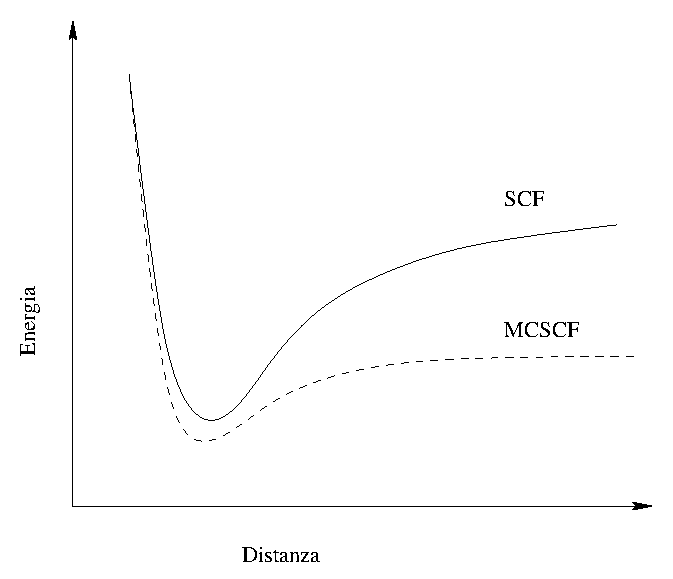
\includegraphics{immagini/SCF-MCSCF.eps} 
\vspace{0.3cm}
\end{center}

Possiamo migliorare la trattazione ipotizzando che la funzione sia descritta
da una combinazione lineare di stati, aggiungendo l'antilegame
\beq
\varphi_2=N_2 \left( 1s_a - 1s_b \right)
\eeq
e scrivendo quindi la funzione d'onda MC
\beq
\Psi_{MC} = c_1 \Phi_1 + c_2 \Phi_2
\eeq
dove
\beq
\Phi_2 = \varphi_2(1) \varphi_2(2) \frac{\alpha \beta - \beta \alpha}{\sqrt{2}}
\eeq
Questa funzione presenta una combinazione, variabile con la distanza, tra le
componenti covalente e ionica, e mostra il corretto comportamento asintotico.

In questo semplice caso, due elettroni vengono distribuiti
su 2 orbitali. Purtroppo anche in molecole semplici, come ossigeno e
azoto, il numero di orbitali e di elettroni con cui trattare risulta
abbastanza elevato. Questo si traduce in una eccessiva complessit\`a computazionale,
nel caso in cui lo scopo fosse una trattazione completa delle possibili distribuzioni
elettroniche. Questa modalit\`a di risoluzione, denominata Full-CI, prende in
considerazione tutte le possibili distribuzioni degli elettroni negli orbitali,
ed \`e la tecnica che fornisce il miglior risultato, per una data
base spinorbitalica. Sebbene ideale, questa strategia \`e raramente 
percorribile proprio a causa dell'eccessivo peso computazionale anche su molecole
piccole.

Al fine di semplificare, e di aprire la possibilit\`a di trattare molecole
di maggiori dimensioni senza pregiudicare il risultato ottenuto, si \`e
optato per includere all'interno della funzione d'onda solo quei determinanti
che si ritengono necessari alla descrizione della molecola. Si parla in questo caso di funzioni
di tipo Multi Reference. Lo schema di selezione dei determinanti da considerare
delinea il metodo multireference scelto.
Uno dei pi\`u noti metodi di selezione, il CAS (Complete Active Space) prevede la
suddivisione dello spazio orbitalico in 3 insiemi: 
\begin{itemize}
\item orbitali virtuali, sempre vuoti
\item orbitali attivi, riempiti in tutti i modi possibili (0, 1, 2
elettroni)
\item orbitali di core, completamente riempiti.
\end{itemize}

Il metodo si basa sulla semplificazione di considerare tutte le possibili
disposizioni degli elettroni solo internamente allo spazio degli
orbitali attivi. Questo riduce la complessit\`a computazionale, e al
tempo stesso tenta di introdurre i maggiori contributi correlativi rispetto
alla semplice funzione HF.

\subsection{Metodo MCSCF e seconda quantizzazione}

Si abbia un set spinorbitalico $ \left\{ \psi_1 \psi_2
\ldots \psi_{n} \right\}$. Usando tali spinorbitali, \`e possibile costruire
un generico determinante di Slater per 3 elettroni
\beq
\Phi = \detsl{\psi_1 \psi_2 \psi_5}
\eeq
Definiamo ora gli operatori di creazione e distruzione, la cui azione
rispettivamente \`e l'aggiunta o la rimozione di uno spinorbitale ad un
determinante, secondo le seguenti regole: per il distruttore, indicato con
la simbologia $\destr{i}$, se lo spinorbitale bersaglio $i$ \`e presente
\beqas
\destr{i}
\detsl{\psi_1,\psi_2,\ldots,\psi_{i-1},\psi_i,\psi_{i+1},\ldots,\psi_{2n}} & = &
(-1)^{p_i} \detsl{\psi_1,\psi_2,\ldots,\psi_{i-1},\psi_{i+1},\ldots,\psi_{2n}}
\eeqas
dove $p_i$ \`e il numero di trasposizioni necessarie a portare lo spinorbitale
bersaglio $i$ in prima posizione nel determinante.
Nel caso lo spinorbitale sia assente, il risultato \`e zero.

Per l'operatore di creazione, indicato con la simbologia $\constr{i}$, se
lo spinorbitale bersaglio $i$ \`e assente
\beqas
\constr{i} \detsl{\psi_1 \psi_2 \ldots } & = &
\detsl{\psi_i \psi_1 \psi_{2} \ldots }
\eeqas
in caso contrario (spinorbitale gi\`a presente), il risultato \`e zero.

\`E utile ricordare le regole di anticommutazione per gli operatori di
creazione e distruzione
\beqas
\constr{i}\constr{j}+\constr{j}\constr{i} = 0 \\
\destr{i}\destr{j}+\destr{j}\destr{i} = 0 \\
\constr{i}\destr{j}+\destr{j}\constr{i} = \delta_{ij}
\eeqas
come anche l'operatore di eccitazione/diseccitazione $\constr{i}\destr{j}$ che
sostituisce in un determinante lo spinorbitale $\psi_j$ con $\psi_i$
\beq
\constr{i}\destr{j} \detsl{\psi_1 \psi_2 \ldots \psi_j \ldots \psi_n} =
\detsl{\psi_1 \psi_2 \ldots \psi_i \ldots \psi_n}
\eeq
Possiamo anche definire un operatore spin traced
\beq
E_{ij} = \left( \constr{i\alpha}\destr{j\alpha} +
\constr{i\beta}\destr{j\beta} \right)
\eeq
che si riferisce agli orbitali molecolari spaziali,
indipendentemente dal fattore di spin.

Valgono le propriet\`a
\begin{itemize}
\item $ \left[ E_{ij}, E_{kl} \right] = E_{il}\delta_{jk} -
E_{kj}\delta_{il} $
\item $ E^{+}_{ij} = E_{ji} $
\end{itemize}

\subsection{Operatori in seconda quantizzazione}

Mediante il formalismo della seconda quantizzazione, \`e possibile
scrivere gli operatori quantistici secondo un differente approccio.
Un generico operatore monoelettronico pu\`o essere espanso sulla base di
operatori di creazione e distruzione
$$
\hat{F} = \sumidx{i,j} F_{ij} \constr{i}\destr{j}
$$
dove $F_{ij}$ \`e l'elemento di matrice
$$
F_{ij} = \int \! \psii^{*}(x)\hat{F}(x)\psij(x) \: dx
$$

Utilizzando gli operatori $E_{ij}$ si pu\`o ottenere
$$
\hat{F} = \sumidx{i,j} F_{ij}E_{ij}
$$
dove gli indici $i$ e $j$ ora sono indici orbitalici puramente spaziali
e l'integrale $F_{ij}$ \`e ora definito su una base spaziale.

Analogamente possiamo definire un operatore bielettronico
$$
\hat{G} = \sumidx{i,j,k,l} g_{ijkl} \constr{i}\constr{j}\destr{l}\destr{k}
$$
dove $g_{ijkl}$ \`e l'integrale
$$
g_{ijkl} = \int \! \! \! \! \int \! \psii^*(x_1) \psij^*(x_2) \hat{G}(x_1,x_2) \psik(x_1)
\psil(x_2) \, dx_1 dx_2
$$

Sommando sullo spin, dopo alcune manipolazioni, \`e possibile ottenere il
risultato
$$
\hat{G} = \half \sumidx{i,j,k,l} g_{ijkl} \left( E_{ik} E_{jl} -
\delta_{jk} E_{il} \right)
$$
dove, al solito, gli indici corrono ora su orbitali puramente spaziali.

In conclusione, l'hamiltoniano in seconda quantizzazione \`e scrivibile
come
$$
\ham = \sumidx{i,j} h_{ij} E_{ij} + \half \sumidx{i,j,k,l} g_{ijkl}
\left( E_{ik} E_{jl} - \delta_{kj} E_{il} \right)
$$

\subsection{Trasformazione di base}

Al fine di rendere minima l'energia, occorre effettuare una trasformazione 
sia sui coefficienti della nostra funzione MC, sia sulla base spinorbitalica 
su cui costruiamo i vari determinanti.

Le trasformazioni della base spinorbitalica possono essere viste come rotazioni in uno spazio
orbitalico, attuate da un operatore opportuno. Dal momento che la
rotazione non cambia la dimensionalit\`a della base, il risultato
appartiene ancora allo spazio delle funzioni spinorbitaliche di
partenza, e come tale \`e esprimibile come una opportuna combinazione
lineare dei vettori della base iniziale
$$
\mbox{\boldmath $\varphi$}^{\prime} = \mbox{\boldmath $\varphi$}\mathbf{U}
$$
dove {\boldmath $\varphi$} \`e un vettore riga contenente gli spinorbitali di
partenza, {\boldmath $\varphi^{\prime}$} \`e la base ottenuta dalla trasformazione e
$\mathbf{U}$ \`e una matrice unitaria che attua la trasformazione stessa.

Dal momento che viene attuata una trasformazione sulla base, anche gli
operatori di creazione e distruzione andranno incontro ad una trasformazione.
\`E possibile esprimere tale trasformazione attraverso
la relazione
\beq
\constr{i}{}^\prime = e^{\left(-\hat{T}\right)} \constr{i}
e^{\left(\hat{T}\right)}
\eeq
e analogamente per il distruttore. L'operatore $\hat{T}$ \`e
antihermitiano, che pu\`o essere espanso, come operatore
monoelettronico, nella forma
\beq
\hat{T}=\sumidx{i,j}T_{ij}\constr{i}\destr{j}
\eeq
dove i coefficienti $T_{ij}$ definiscono una matrice $\mathbf{T}$ antihermitiana (ovvero
\mbox{$\mathbf{T}^{+} = - \mathbf{T}$})

Si dimostra che \`e possibile trasformare un generico determinante di 
Slater applicando l'operatore $e^{-\hat{T}}$:
\beqas
% 
\ket{m'}= a{'}_i^+ a{'}_j^+ \ldots\vacuum & = &
e^{\left(-\hat{T}\right)} \constr{i} e^{\left(\hat{T}\right)}
e^{\left(-\hat{T}\right)}\constr{j} e^{\left(\hat{T}\right)}\ldots\vacuum
\\
% 
& = & e^{\left(-\hat{T}\right)}\constr{i} \constr{j}\ldots\vacuum \\
%
& = & e^{\left(-\hat{T}\right)}\ket{m}
\eeqas

Dal momento che la trasformazione attuata sugli orbitali
avviene esclusivamente sulla parte spaziale, la matrice di
trasformazione $\mathbf{T}$ \`e partizionata in 4 sottomatrici
\beq
\mathbf{T} = \left(
\begin{array}{cc}
\mathbf{T}_{\alpha\alpha} & \mathbf{T}_{\alpha\beta} \\
\mathbf{T}_{\beta\alpha} & \mathbf{T}_{\beta\beta}
\end{array}
\right)
\eeq

Se, in seguito al cambiamento di base, non si effettua mescolamento tra
orbitali con occupazione $\alpha$ e orbitali con occupazione $\beta$, i
termini delle sottomatrici fuori  diagonale $\mathbf{T}_{\alpha\beta}$ e
$\mathbf{T}_{\beta\alpha}$ sono nulli. Inoltre, dato che le trasformazioni
sono le stesse per lo stesso set spaziale, $\mathbf{T}_{\alpha\alpha} = \mathbf{T}_{\beta\beta}$.
Con queste relazioni, l'operatore $\hat{T}$ risulta
\beqa
%
\hat{T} & = & \sumidx{i,j} \left( T_{ij}^{\alpha\alpha} \constr{i\alpha}
\destr{j\alpha} 
+ T_{ij}^{\alpha\beta} \constr{i\alpha} \destr{j\beta}
+ T_{ij}^{\beta\alpha} \constr{i\beta} \destr{j\alpha}
+ T_{ij}^{\beta\beta} \constr{i\beta} \destr{j\beta} \right) \nonumber \\
%
& = & \sumidx{i,j} T_{ij} \left( \constr{i\alpha} \destr{j\alpha} +
\constr{i\beta} \destr{j\beta} \right) \nonumber \\
%
& = & \sumidx{i,j} T_{ij}E_{ij}
\eeqa
supponendo la matrice antihermitiana $\mathbf{T}$ reale, si avr\`a $T_{ij} = -T_{ji}$ e
quindi
\beq
\hat{T} = \sumidx{i>j} T_{ij}\left(E_{ij} - E_{ji}\right) 
= \sumidx{i>j} T_{ij} E_{ij}^-
\eeq
dove con l'ultimo termine si esprime una scrittura abbreviata.

\subsection{Metodo risolutivo Newton-Raphson}

L'ottimizzazione di una funzione d'onda multiconfigurazionale prevede
di modificare sia gli orbitali base, sia i coefficienti della combinazione
lineare di determinanti.
Uno dei metodi di risoluzione \`e conosciuto come metodo Newton-Raphson, o
metodo NR: l'assunto di partenza \`e considerare l'energia del sistema $E$ come
funzione di un vettore di parametri $\mathbf{p}$, e quindi espandere
tale dipendenza in serie di Taylor attorno un punto $\mathbf{p}_0$.
Si avr\`a
\beq
E(\mathbf{p}) = E(\mathbf{p}_0) + \sumidx{i} \left( \frac{\partial E}{\partial
p_i}\right)_{\mathbf{p}_0} p_i + \half \sumidx{i,j} p_i \left( \frac{\partial^2 E}{\partial
p_i \partial p_j} \right)_{\mathbf{p}_0} p_j + \ldots
\eeq
che in notazione matriciale diventa
\beq
E(\mathbf{p}) = E(\mathbf{p}_0) + \mathbf{g}^+\mathbf{p} + \half
\mathbf{p}^+\mathbf{H}\mathbf{p} + \ldots
\eeq
dove $\mathbf{g}$ \`e un vettore detto \textit{gradiente energia} e
$\mathbf{H}$ \`e la \textit{matrice Hessiana} dell'energia.

Affinch\`e si abbia un minimo, la derivata prima dell'energia rispetto 
a tutti i parametri deve essere zero, ovvero il vettore gradiente nullo.
Per risolvere tale problema, si ricorre ad una procedura iterativa 
che prevede la risoluzione dell'equazione lineare
\beq
\mathbf{g} + \mathbf{Hp} = \mathbf{0} 
\eeq

\subsection{Ottimizzazione dei parametri e degli orbitali}

L'ottimizzazione dei parametri e degli orbitali passa attraverso l'uso
di operatori unitari. \`E gi\`a stato presentato l'operatore $\hat{T}$, 
che attua una rotazione dello spazio orbitalico. Analogamente,
\`e possibile definire un operatore unitario $\hat{S}$ che attua una
trasformazione sui coefficienti della combinazione lineare.

L'energia dello stato MC $\ket{0}$ sar\`a quindi definita
\beq
E(\mathbf{T},\mathbf{S}) =
\braket{0}{e^{\left(-\hat{S}\right)}e^{\left(-\hat{T}\right)}\ham e^{\left(\hat{T}\right)}e^{\left(\hat{S}\right)}}{0}
\eeq
Espandendo con l'identit\`a di Glauber\footnote{Ricordiamo l'identit\`a di Glauber 
\beqas
e^{\hat{A}}\hat{B}e^{-\hat{A}} & = & \hat{B} + \left[ \hat{A} , \hat{B}
\right] + \frac{1}{2!} \left[ \hat{A} , \left[ \hat{A} , \hat{B} \right]
\right] + \frac{1}{3!} \left[ \hat{A} , \left[ \hat{A} , \left[ \hat{A} ,
\hat{B} \right] \right] \right] + \ldots
\eeqas
} tale espressione, si ottiene
\beqas
E(\mathbf{T},\mathbf{S}) & = & \left\langle 0 \left| \ham + \left[\ham,\hat{T}\right] 
+ \left[\ham,\hat{S}\right] 
+ \half \left[ \left[ \ham,\hat{T}\right],\hat{T}\right] \right. \right. \\
& & \left. \left. + \half \left[ \left[ \ham,\hat{S}\right],\hat{S}\right]
+ \left[ \left[ \ham,\hat{T}\right],\hat{S}\right]
+ \ldots \right| 0 \right\rangle
\eeqas

Il primo termine rende conto dell'energia di ordine zero
$E(\mathbf{0},\mathbf{0})$. Il successivo pu\`o essere sviluppato
\beqas
\braket{0}{\left[\ham,\hat{T}\right]}{0} & = & \sumidx{i,j} T_{ij}
\braket{0}{\left[\ham,E_{ij}\right]}{0} \\
%
& = & \sumidx{i,j} T_{ij} g_{ij}^{(o)}
\eeqas
dove abbiamo posto
\beq
g_{ij}^{(o)} = \braket{0}{\left[\ham,E_{ij}\right]}{0}
\eeq
Il simbolo $(o)$ indica che la trasformazione \`e a carico degli
orbitali.

Ora \`e necessario ottenere l'operatore per la trasformazione a
carico dei coefficienti. Sia innanzitutto definito l'operatore di rotazione
sui coefficienti $\hat{S}$ come
\beq
\hat{S} = \sumidx{K\neq0} S_{K0} \left(\ket{K}\bra{0} - \ket{0}\bra{K}
\right)
\eeq
dove $\ket{K}$ sono generici stati, espansi sulla medesima base
spinorbitalica, tali da essere ortogonali tra loro.

Svolgendo opportunamente il commutatore
\beq
\braket{0}{\left[\ham,\hat{S}\right]}{0} =
\sumidx{K\neq0}S_{K0} \left( \braket{0}{\ham}{K} + \braket{K}{\ham}{0}
\right)
\eeq
che con autofunzioni reali, per hermitianit\`a, conduce ad ottenere
\beq
g_K^{(c)} = 2 \braket{0}{\ham}{K}
\eeq
vettore che esprime la derivata prima effettuata su una
variazione dei coefficienti della funzione MC.

\`E possibile procedere in modo analogo ricavando la matrice
\textit{hessiana}, responsabile della trasformazione al secondo ordine.
Si otterranno 3 contributi: un contributo (oo) di trasformazione sugli 
orbitali, un contributo (cc) di trasformazione sui coefficienti e 
un contributo (co) = (oc) di variazione accoppiata orbitali-coefficienti.

Ora, riprendendo e riadattando
\beqas
\mathbf{g} + \mathbf{Hp} = \mathbf{0} \\
\mathbf{Hp} = - \mathbf{g}
\eeqas
si pu\`o scrivere, in definitiva
\beq
\left(
\begin{array}{cc}
\half \mathbf{H}^{(cc)} & \half \mathbf{H}^{(co)} \\
\left( \half \mathbf{H}^{(co)} \right)^+ & \half \mathbf{H}^{(oo)} \\
\end{array}
\right) 
\left(
\begin{array}{c}
\mathbf{S} \\
\mathbf{T} \\
\end{array}
\right) = -
\left(
\begin{array}{c}
\half \mathbf{g}^{c} \\
\half \mathbf{g}^{o} \\
\end{array}
\right)
\eeq

Il metodo Newton-Raphson prevede la risoluzione iterativa di questo
sistema o analoghi (al fine di semplificare il metodo computazionale),
tuttavia richiede che il vettore di guess per il processo iterativo
sia sufficientemente vicino al minimo locale verso cui si vuole convergere. In
caso contrario, il metodo pu\`o convergere molto lentamente o addirittura
divergere. Sono quindi necessarie procedure per identificare una zona
di minimo, in cui definire in modo approssimativo un vettore di guess.

\subsection{Metodo Super-CI}
Un metodo alternativo all'approccio Newton-Raphson \`e il cosiddetto
metodo Super-CI.
Tale metodo prevede di annullare l'interazione con gli stati
monoeccitati mediante una procedura iterativa.
Per risolvere tale problema, si costruisce una funzione Super-CI come
$$
\ket{SCI} = \ket{0} + \sumidx{p>q}t_{pq}E_{pq}^-\ket{0}
$$
dove $E_{pq}^- = E_{pq} - E_{qp}$.
La funzione d'onda SCI \`e una combinazione di uno stato base MC e delle
sue eccitazioni. Il metodo prevede di ottenere la convergenza quando
$\braket{0}{\ham}{E_{pq}^- 0} = 0$ come affermato dal teorema di Brillouin,
esteso a casi multireference (Cfr. \cite{ijqc-2-1968-307}).

Una particolarit\`a del metodo risiede nella non ortogonalit\`a delle
singole eccitazioni
\beqas
S_{pq,rs} &=& \integral{E_{pq}^-0}{E_{rs}^-0} \\
&=& \braket{0}{E_{qp}^-E_{rs}^-}{0} \\
& \neq & \delta_{pq,rs}
\eeqas
le funzioni non sono nemmeno normalizzate ($S_{pq,pq} \neq 1$).

Gli elementi di matrice dell'hamiltoniano hanno la forma
\beqas
\braket{0}{\ham}{pq} &=& \braket{0}{\ham E_{pq}^-}{0} = w_{pq} \\
\braket{pq}{\ham}{rs} &=& \braket{0}{E_{qp}^-\ham E_{rs}^-}{0} = d_{pq,rs}
\eeqas
L'equazione secolare da risolvere sar\`a quindi
$$
\left(
\begin{array}{cc}
E_{MC} & \mathbf{w}^+ \\
\mathbf{w} & \mathbf{d}
\end{array} \right)
\left(
\begin{array}{c}
1 \\
\mathbf{t} \\
\end{array}
\right)
= E_{SCI}
\left(
\begin{array}{cc}
1 & \mathbf{0} \\
\mathbf{0} & \mathbf{S}
\end{array}
\right)
\left(
\begin{array}{c}
1 \\
\mathbf{t} \\
\end{array}
\right)
$$
che pu\`o anche essere riscritta come
$$
\left(
\begin{array}{cc}
0 & \mathbf{w}^+ \\
\mathbf{w} & \mathbf{d}-E_{MC}\mathbf{S}
\end{array} \right)
\left(
\begin{array}{c}
1 \\
\mathbf{t} \\
\end{array}
\right)
= \left( E_{SCI} - E_{MC} \right)
\left(
\begin{array}{cc}
1 & \mathbf{0} \\
\mathbf{0} & \mathbf{S}
\end{array}
\right)
\left(
\begin{array}{c}
1 \\
\mathbf{t} \\
\end{array}
\right)
$$

Il metodo Super-CI converge sempre in un minimo locale, al contrario del
metodo Newton-Raphson che pu\`o convergere anche in punti di sella.



\chapter{Teoria perturbativa NEV-PT}

\section{Introduzione}

\`E stato possibile vedere come la migliore accuratezza possibile per
un dato sistema sia ottenibile, in linea di principio, con una espansione
Full-CI su una base data. Questo approccio \`e percorribile con difficolt\`a 
a causa della complessit\`a computazionale eccessiva. Per porre
rimedio a tale limitazione, definire uno schema di selezione per gli orbitali
pu\`o essere una buona approssimazione, se tale schema prende in
considerazione gli orbitali maggiormente significativi.
Questo approccio multireference pu\`o essere eventualmente migliorato 
applicando una correzione perturbativa alle funzioni d'onda e alle relative
energie.

Le teorie perturbative multireference (MRPT) costituiscono uno strumento
prezioso per il calcolo dell'energia di correlazione in molecole di piccole
e medie dimensioni. Sebbene i primi tentativi di formulare teorie MRPT
risalgano ad oltre trent'anni fa (Cfr. \cite{rmp-39-1967-771},
\cite{jcp-58-1973-5745}) \`e solamente nell'ultima decade che tali strumenti
sono diventati di utilizzo comune. Lo scopo delle teorie perturbative
multireference \`e di fornire uno strumento agile e preciso, che ricalchi il
famoso approccio M{\o}ller-Plesset (Cfr. \cite{pr-46-1934-618}) per il caso
di una funzione d'onda monodeterminantale.
Come \`e noto, nel caso di una molecola che sia ben descritta da un singolo
determinante di Slater (come la maggior parte delle molecole nello stato
fondamentale ed alla geometria di equilibrio) l'applicazione della teoria
perturbativa al secondo ordine nell'energia, nell'approccio
M{\o}ller-Plesset (MP2) fornisce spesso oltre il 90 \% dell'energia di
correlazione.
L'hamiltoniano di ordine zero della teoria MP \`e molto semplice, e consiste
nell'operatore di Fock a $n$ particelle
\beq
\ham_0 = \sumonen{i} \fock(i)
\eeq
Applicando quanto esposto nella sezione \ref{sec:perturbazione} si ottiene
subito, al secondo ordine
\beq
E_0^{(2)} = - \sum_{i,j}^{\mbox{occ}} \sum_{r,s}^{\mbox{virt}} \frac{\left|
\interact{rs}{ij}\right|^{2}}{\epsilon_r + \epsilon_s - \epsilon_i -
\epsilon_j }
\eeq

Nel caso di una MRPT, la funzione d'onda di ordine zero \`e multireference,
ossia una combinazione lineare di determinanti di Slater. Di conseguenza,
non \`e ovvio come si possa arrivare ad una efficace definizione
dell'hamiltoniano di ordine zero. I vari metodi MRPT rientrano in due
distinte categorie: la prima viene indicata come "\textit{perturb then diagonalize}"
e si basa sulla possibilit\`a di costruire un hamiltoniano efficace,
definito perturbativamente, che sar\`a diagonalizzato (Cfr. \cite{rmp-39-1967-771} e
\cite{jpa-18-1985-809})

La seconda categoria, nota invece come "\textit{diagonalize then perturb}",
parte da una funzione d'onda variazionale ed applica a questa la teoria
perturbativa. A questa categoria appartengono le tecniche CIPSI, iniziate a
Parigi da Huron \textit{et al.} (Cfr. \cite{jcp-58-1973-5745}) e
successivamente proseguite a Pisa (Cfr. \cite{jcc-8-1987-39}) e 
Ferrara (Cfr. \cite{ijqc-60-1996-167}, \cite{tca-98-1997-57} e
\cite{tca-98-1997-117}), le quali si basano sull'uso
dei semplici determinanti di Slater come funzioni perturbatrici, e la
tecnica CASPT2 (Cfr. \cite{jpc-94-1990-5483} e \cite{jcp-96-1992-1218}) che
utilizza invece funzioni "contratte" (particolari combinazioni di
determinanti) nella teoria perturbativa.

Tra le propriet\`a pi\`u desiderabili di una teoria perturbativa
multireference citiamo le seguenti:
\begin{itemize}
\item size consistence (o strict separability). Si vorrebbe che nel calcolo
di un sistema consistente di due parti non interagenti (AB) l'energia
risultasse uguale alla somma delle due parti (E$_{AB} = $E$_A + $E$_B$)
\item assenza di "intruder states". Le funzioni che correggono la funzione
d'onda all'ordine zero dovrebbero avere energie ben distinte da quella della
funzione d'ordine zero stessa, in maniera da evitare divergenza. La semplice
formula di M{\o}ller-Plesset soddisfa questo requisito: le funzioni
perturbatrici sono i semplici determinanti di doppia sostituzione
$\Phi_{ij}^{rs}$ che, data la forma adottata per $\ham_0$ hanno come energia
$E_0 + \epsilon_r + \epsilon_s - \epsilon_i - \epsilon_j$, ben distinta da
$E_0$.
\item L'accuratezza nel calcolo degli stati elettronicamente eccitati
dovrebbe essere comparabile con quella ottenuta per lo stato fondamentale.
\end{itemize}

Per svariati motivi, le teorie perturbative fin qui citate falliscono
nell'esaudire uno o pi\`u di questi requisiti.
L'approccio perturbativo $n$-Electron Valence Perturbation Theory (NEV-PT)
(Cfr. \cite{jcp-114-23-2001-10252}), sviluppato in collaborazione tra il
nostro gruppo di Ferrara e quello del Prof. Malrieu dell'universit\`a di
Tolosa, risolve in modo formale sia le necessit\`a di size-consistency, sia
il problema di stati intrusi, che sono le principali necessit\`a di una
teoria perturbativa, ed inoltre si comporta come un approccio
M{\o}ller-Plesset se applicato ad una funzione
single reference.

Nello sviluppo dell'approccio NEV-PT si \`e giocato su due variabili:
\begin{itemize}
\item il grado di contrazione dello spazio perturbatore
\item la scelta dell'hamiltoniano
\end{itemize}

In alcuni casi, si \`e fatto uso dell'hamiltoniano proposto da Dyall (Cfr.
\cite{jcp-102-1995-4909}). Tale hamiltoniano risolve il problema formale che
nasce nel momento in cui la funzione d'onda multireference all'ordine zero
incorpora effetti di interazione bielettronica, mentre qualsiasi trattazione
perturbativa che si rifaccia all'hamiltoniano M{\o}ller-Plesset fa uso di
un hamiltoniano puramente monoelettronico.
L'Hamiltoniano di Dyall \`e un hamiltoniano approssimato bielettronico, che
quindi si presta meglio, dal punto di vista formale, alle trattazioni a
seguire.

\section{Teoria}

La teoria perturbativa NEV-PT necessita di una funzione all'ordine zero
definita su uno spazio CAS
\beq
\Psi_m^{(0)} = \sumidx{I \in \mbox{CAS}} C_{I,m} \ket{I}
\eeq
ottenuto diagonalizzando $\ham$ nello spazio CAS
\beq
\proj{\mbox{CAS}}\ham\proj{\mbox{CAS}}\ket{\Psi_m^{(0)}} = E_m^{(0)} \ket{\Psi_m^{(0)}}
\eeq
dove $\proj{CAS}$ \`e il proiettore all'interno dello spazio CAS
\beq
\proj{\mbox{CAS}} = \sum_{M}^{\mbox{CAS}} \ket{\mbox{M}} \bra{\mbox{M}}
\eeq
Le funzioni perturbatrici sono esterne a tale spazio, e quelle di interesse
per il metodo NEV-PT sono classificabili nel seguente schema: la funzione
d'onda all'ordine zero \`e scrivibile come un prodotto antisimmetrizzato di
una parte inattiva con $n_c$ elettroni e di una funzione
multireference di valenza con $n_v$ elettroni
\beq
\ket{\Psi_m^{(0)}} = \ket{\Phi_c \Psi_m^v}
\eeq
e in modo analogo le funzioni perturbatrici avranno la forma
\beq
\ket{\Phi_l^{-k} \Psi_{\mu}^{v+k}}
\eeq
dove $k$ \`e il numero di elettroni rimossi dallo spazio inattivo e
introdotti nello spazio attivo ed $l$ denota gli orbitali inattivi (core + virtuale).
Al secondo ordine di perturbazione $k$ \`e
compreso tra -2 e 2.
Richiediamo inoltre che non esista interazione tra due funzioni
perturbatrici appartenenti alla medesima classe, individuata dagli indici
$k$ e $l$. In altri termini, deve valere
\beq
\braket{\Phi_l^{-k} \Psi_{\mu}^{v+k}}{\ham}{\Phi_l^{-k} \Psi_{\nu}^{v+k}} =
0 \qquad \mbox{per }\mu \neq \nu
\eeq

Il modo migliore per definire tali funzioni perturbatrici \`e espanderle su
una base di uno spazio $S_l^k$  individuato dai determinanti con la
medesima parte inattiva $\Phi_l^{-k}$ e tutte le possibili parti attive
$\Phi_I^{+k}$. In altri termini, tale spazio avr\`a come base il set di
determinanti
\beq
\left\{ \Phi_l^{-k} \Phi_I^{+k} \right\}
\eeq
e le funzioni perturbatrici saranno combinazioni lineari opportune
all'interno di tale spazio. Questo tipo di approccio sfrutta l'intera
dimensionalit\`a offerta dallo spazio perturbatore $S_l^k$ e viene denominato
\textbf{totalmente non contratto}.

Per ottenere le funzioni pertubatrici sar\`a sufficiente diagonalizzare
l'hamiltoniano all'interno di tale spazio
\beq
\label{eqn:teoria1_1}
\proj{S_l^k}\ham\proj{S_l^k} \ket{\Phi_l^{-k} \Psi_{\mu}^{v+k}} = E_{l,\mu}
\ket{\Phi_l^{-k} \Psi_{\mu}^{v+k}}
\eeq
tuttavia tale procedura \`e computazionalmente pesante. Una possibile
semplificazione si ottiene con l'utilizzo dell'hamiltoniano di Dyall,
che \`e definito nel modo seguente
\beqa
\ham^D &=& \ham^D_i + \ham^D_v \\
\ham^D_i &=& \sumidx{i} \epsilon_i \constr{i} \destr{i} + \sumidx{r}
\epsilon_r \constr{r} \destr{r} + C \\
\ham^D_v &=& \sumidx{ab} h_{ab}^{\mbox{eff}} \constr{a} \destr{b} +
\frac{1}{2} \sumidx{abcd} \integral{ab}{cd} \constr{a}\constr{b}
\destr{d}\destr{c}
\eeqa
dove con indici $i,j,\ldots$, $a,b,\ldots$, $r,s,\ldots$ si indicano
rispettivamente orbitali di core, attivi e virtuali e definiamo 
$ h_{ab}^{\mbox{eff}} = \braket{a}{h+\sumidx{i}\left( J_i - K_i \right)}{b}$.

$\ham^D$ gode della propriet\`a di comportarsi esattamente come l'hamiltoniano
vero all'interno dello spazio CAS, dopo un'appropriata scelta della costante C.
Come conseguenza, tale hamiltoniano possiede gli stessi autovalori e gli stessi
autovettori dell'hamiltoniano vero proiettato all'interno dello spazio CAS.

%La struttura dell'hamiltoniano di Dyall permette inoltre di considerare che,
%nell'equazione \ref{eqn:teoria1_1} relativa a questo hamiltoniano, le energie
%$E_{l,\mu}$ possono essere ricavate da una traslazione energetica
%appropriata (e determinata esclusivamente dalla distribuzione elettronica
%della parte inattiva) rispetto al valore $E_{\mu,k}$ restituito dalla
%relazione
%\beq
%\ham_v^D \ket{ {\Psi^{\prime}}_{\mu}^{v+k}} = E_{l,\mu} \ket{
%{\Psi^{\prime}}_{\mu}^{v+k}}
%\eeq
%che interessa esclusivamente la parte attiva, in quanto la parte inattiva
%pu\`o essere operata a parte in virt\`u della forma dell'operatore di Dyall,
%e comporta appunto una traslazione energetica, come enunciato poco sopra.

\subsection{Approccio partially contracted}

L'approccio sopra enunciato fa uso dell'intera dimensionalit\`a degli spazi
$S_l^k$. Una alternativa computazionalmente pi\`u semplice \`e l'utilizzo di
un sottospazio di $S_l^k$, definito dall'applicazione di un operatore di perturbazione
$\perturb$ alle funzioni d'onda CAS $\Psi_m^{(0)}$. \`E possibile
dimostrare che l'operatore di perturbazione \`e scrivibile come una somma di
contributi
\beqa
\perturb^u &=& \perturb^{(0)} + \perturb^{(+1)} + \perturb^{(-1)} +
\perturb^{(+2)} + \perturb^{(-2)} + \perturb^{\prime(+1)} \nonumber \\
& & + \perturb^{\prime(-1)} + \perturb^{\prime(0)}
\eeqa

Ciascun contributo \`e costituito da una somma di termini dell'hamiltoniano,
i quali, applicati a $\Psi_m^{(0)}$, generano funzioni appartenenti ai vari
spazi $S_l^k$. Nel complesso, tali funzioni generano sottospazi di
$S_l^k$, che indicheremo con $\overline{S}_l^k$.

Ad esempio, l'operatore $\perturb^{(+1)}$, che rappresenta la componente
perturbativa il cui effetto \`e di promuovere un elettrone dagli orbitali di
core a quelli attivi e un altro elettrone dagli orbitali di core ai
virtuali, sar\`a
\beq
\perturb^{(+1)} = \sumidx{i<j} \sumidx{r} \sumidx{a} \interact{ra}{ji}
\constr{r}\constr{a}\destr{i}\destr{j} = \sumidx{i<j}\sumidx{r}
\perturb_{ijr}^{(+1)}
\eeq
e ciascuno degli elementi di $\perturb_{ijr}^{(+1)}$ genera funzioni del
tipo $\ket{\Phi_l^{-1} \constr{a} \Psi_{m}^{v}}$ che appartengono allo spazio
$S_l^{(+1)}$. Il set di funzioni $\left\{ \ket{\Phi_l^{-1} \constr{a} \Psi_{m}^{v}} \right\}$
genera uno spazio $\overline{S}_l^{+1}$ la cui dimensionalit\`a \`e uguale
al numero degli orbitali attivi. La diagonalizzazione dell'hamiltoniano
completo o di Dyall in ciascuno di questi sottospazi fornisce le funzioni
perturbatrici necessarie, ottimizzate variazionalmente, e le relative
energie. Tale risoluzione pu\`o essere applicata a qualsiasi componente sopra
presentato, e generer\`a funzioni che apparterranno ad opportuni sottospazi.

Una particolarit\`a \`e fornita dall'operatore $\perturb_{ijrs}^{(0)}$. Lo
spazio ridotto $\overline{S}_l^{0}$, per una data scelta degli indici $i,j,r,s$,
contiene una sola funzione
significativa per il calcolo perturbativo, che descrive una doppia eccitazione
dallo spazio di core allo spazio virtuale. 
L'energia associata a tale funzione perturbatrice quando si adoperi
l'hamiltoniano di Dyall non \`e altro che l'energia della funzione CAS
corretta con l'aggiunta del termine $\epsilon_r + \epsilon_s - \epsilon_i -\epsilon_j$,
ovvero la differenza delle energie degli orbitali interessati all'eccitazione.

La correzione perturbativa al primo ordine della funzione d'onda
per tale caso sar\`a data da
\beqa
\Psi_{m}^{(1)}(\perturb^{(0)}) &=& - \sumidx{i<j} \sumidx{r<s} 
\ket{\constr{r}\constr{s}\destr{i}\destr{j} \Phi_{c} \Psi_m^v} \nonumber \\
& & \times \frac{\braket{\constr{r}\constr{s}\destr{i}\destr{j} \Phi_{c}
\Psi_m^v}{\ham}{\Psi_m^{(0)}}}{\epsilon_r + \epsilon_s - \epsilon_i
- \epsilon_j}
\eeqa

e conseguentemente la correzione al secondo ordine per l'energia sar\`a data
dal valore
\beq
\braket{\Psi_{m}^{(0)}}{\ham}{\Psi_{m}^{(1)}(\perturb^{(0)})}
\eeq
ovvero
\beq
E_{m}^{(2)}(\perturb^{(0)}) = - \sumidx{i<j} \sumidx{r<s} \frac{\left| \left< rs \left|
\right| ji \right> \right|^2}{\epsilon_r + \epsilon_s -
\epsilon_i-\epsilon_j}
\eeq

che non \`e altro che il contributo M{\o}ller-Plesset MP2, nel caso di una funzione HF.
La teoria NEV-PT di conseguenza si riduce ad una trattazione M{\o}ller-Plesset
nel momento in cui lo spazio attivo non esista (come nel caso
dell'approssimazione monodeterminantale,
a cui la perturbazione MP2 fa riferimento).

Nel caso dei termini di $\perturb$ che coinvolgano lo spazio attivo, la
trattazione \`e pi\`u complessa. Le funzioni saranno del tipo $\ket{\constr{r}
\destr{i}\destr{j}\Phi_c \Psi_{\mu}^{(+1)}}$, dove la parte attiva \`e
caratterizzata da un elettrone in pi\`u rispetto alla funzione CAS.
La correzione alla funzione d'onda al primo ordine sar\`a
\beqa
\Psi_{m}^{(1)}(\perturb^{(+1)}) &=& - \sumidx{i<j} \sumidx{r} \sumidx{\mu}
\ket{\constr{r}\destr{i}\destr{j}\Phi_c \Psi_{\mu}^{(+1)}} \nonumber \\ 
&\times& \frac{\braket{\constr{r}\destr{i}\destr{j}\Phi_c \Psi_{\mu}^{(+1)}}{\ham}{\Psi_m^{(0)}}}{E_{\mu}^{(+1)} - E_m^{(0)} + \epsilon_r - \epsilon_i - \epsilon_j}
\eeqa

Si dovr\`a quindi calcolare una interazione del tipo
\beq
\braket{\constr{r}\destr{i}\destr{j}\Phi_c\Psi_{\mu}^{(+1)}}
{\ham}{\Psi_m^{(0)}}
\eeq

Siccome l'interazione avviene esclusivamente attraverso
il termine perturbatore, risulter\`a
\beq
\braket{\constr{r}\destr{i}\destr{j}\Phi_c\Psi_{\mu}^{(+1)}} {\perturb^{(+1)}_{ijr}}{\Psi_m^{(0)}}
\eeq
dalla quale, per svolgimento dell'operatore e dopo alcuni passaggi, si
otterr\`a
\beqas
\integral{\constr{r}\destr{i}\destr{j}\Phi_c\Psi_{\mu}^{(+1)}}{\sumidx{a}\interact{ra}{ji}\constr{r}\destr{i}\destr{j}\Phi_c\constr{a}\Psi_m^v} = 
\eeqas
\beqa
&=& \sumidx{a} \interact{ra}{ji} \integral{\Psi_\mu^{(+1)}}{\constr{a}\Psi_m^v} \nonumber \\
&=& \sumidx{a} \interact{ra}{ji} S_{\mu a} \stackrel{\mbox{\tiny def}}{=}
\interact{r\mu}{ji}
\eeqa

Nella formula precedente, il termine $\sumidx{a} \interact{ra}{ji} S_{\mu a}$ \`e stato ridotto
ad un solo integrale bielettronico efficace che coinvolge una ``quasi-particella'' nella valenza.
Di conseguenza, tale termine pu\`o essere scritto tramite il semplice integrale
$\interact{r\mu}{ji}$ e la correzione perturbativa al secondo ordine 
sull'energia sar\`a
\beq
E_{(+1),m}^{(2)} = - \sumidx{i<j} \sumidx{r} \sumidx{\mu}
\frac{\left| \interact{r\mu}{ji} \right| ^2}{E^{(+1)}_{\mu} - E_m^{(0)} + \epsilon_r -
\epsilon_i - \epsilon_j }
\eeq

Analogamente, gli altri contributi rappresentano l'inserimento di
``quasi-buche'' o ``quasi-coppie'' all'interno dello strato di valenza.
Si otterranno quindi una serie di contributi all'energia per la correzione
perturbativa, che saranno centrali nell'analisi dei dati attuata nel
seguito di questa tesi.

\subsection{Approccio strongly contracted}

Un'ulteriore semplificazione pu\`o essere introdotta riducendo ancora la 
dimensione dello spazio perturbativo. Ogni termine $\hat{\mathcal{V}}$,
come \`e stato visto in precedenza, genera un sottospazio perturbativo la
cui dimensione dipende in modo diretto da quella dello spazio attivo
selezionato. \`E tuttavia possibile utilizzare gli operatori perturbativi in
modo da fornire una sola funzione appartenente a ciascuno
spazio, ed attuare la trattazione esclusivamente con tali funzioni.

Al fine di ottenere ci\`o, nel caso di esempio $\perturb^{(+1)}$, avremo
\beq
\ket{\phi_{ijr}} = \perturb_{ijr}^{(+1)} \ket{\Psi_m^{(0)}} = \constr{r}
\destr{i} \destr{j} \Phi_c \sumidx{a}\interact{ra}{ji} \constr{a}
\Psi^{v}_{m}
\eeq

Questa funzione d'onda, generalmente non normalizzata, definisce uno spazio
monodimensionale $\tilde{S}_l^k$ che sar\`a considerato al fine della
trattazione perturbativa per la parte $\perturb^{(+1)}$.
La norma di tale funzione assume un significato molto importante, in quanto
\`e direttamente implicata nel trattamento perturbativo, e pu\`o facilmente
essere ottenuta da:
\beqa
N_{ijr} = \integral{\phi_{ijr}}{\phi_{ijr}} &=& \left( \sumidx{a} \interact{ra}{ji}
\ket{\constr{a}\Psi_m^{v}} \right) \left( \sumidx{b} \interact{rb}{ji}
\ket{\constr{b}\Psi_m^v} \right) \nonumber \\
&=& \sumidx{ab} \interact{ra}{ji} \integral{\constr{a} \Psi_m^v}{\constr{b}
\Psi_m^v} \interact{rb}{ji} \nonumber \\
&=& \sumidx{ab} \interact{ra}{ji} \tilde{\rho}_{ba} \interact{rb}{ji}
\eeqa
dove $\tilde{\rho}_{ba} =
\braket{\Psi_m^{(0)}}{\destr{a}\constr{b}}{\Psi_m^{(0)}}$ \`e la matrice
densit\`a ad una buca (legata alla matrice densit\`a ad una particella dalla
relazione $\tilde{\rho}_{ba} = \delta_{ab} - \rho_{ab}$)

Quindi la funzione d'onda normalizzata sar\`a data da 
\beq
\ket{\phi_{ijr}^{\prime}} = \frac{1}{\sqrt{N_{ijr}}} \ket{\phi_{ijr}}
\eeq

Da questa \`e possibile ricavare i coefficienti della correzione perturbativa
al primo ordine:
\beqa
C_{ijr}^{(1)} &=& \frac{\braket{\phi^{\prime}_{ijr}}{\ham}{\Psi_m^{(0)}}}{E_m^{(0)} - E_{ijr}} \nonumber \\
&=& \frac{\braket{\phi^{\prime}_{ijr}}{\perturb_{ijr}^{(+1)}}{\Psi_m^{(0)}}}{E_m^{(0)} - E_{ijr}} \nonumber \\
&=& \frac{\integral{\phi^{\prime}_{ijr}}{\phi_{ijr}}}{E_m^{(0)} - E_{ijr}} \nonumber \\
&=& \frac{\sqrt{N_{ijr}}}{E_m^{(0)} - E_{ijr}}
\eeqa
e di conseguenza la correzione perturbativa all'energia
\beq
E_m^{(2)} = \frac{N_{ijr}}{E_m^{(0)} - E_{ijr}}
\eeq
dove il termine $E_{ijr}$ \`e il valore medio dell'hamiltoniano di Dyall
nella funzione $\ket{\phi^{\prime}_{ijr}}$.


\pagebreak
\chapter{Programmi di calcolo}

Questo capitolo presenter\`a la catena di calcolo utilizzata per implementare
la trattazione \textit{ab initio} che verr\`a esposta nei suoi risultati nel
capitolo \ref{cap:applicazioni}. La catena \`e costituita dai seguenti
programmi
\begin{itemize}
\item \texttt{dalton 1.2}
\item \texttt{gaussian 98}
\item \texttt{ijkldali}
\item \texttt{cipselx}
\item \texttt{cippiS2s}
\item \texttt{koopro4E}
\item \texttt{dypc2}
\end{itemize}

Per le piattaforme di lavoro, si \`e fatto uso di Linux RedHat 7.2 su hardware
sia Intel che AMD. La configurazione Intel comprende un dual-processor 
Intel Pentium III a 1 GHz con 1 Gb di RAM ed un totale di 120 Gb di Hard-Disk
IDE/SCSI. La configurazione AMD comprende invece due macchine, 
un single-processor AMD
Athlon XP 1700+ con 1.5 Gb di RAM ed un totale di 90 Gb di Hard-Disk IDE
e un Athlon XP 1800+ con 1.5 Gb di RAM e 100 Gb totali di Hard-Disk IDE.


\section{Descrizione dei programmi}

\subsection{\texttt{dalton 1.2}}

Il programma \texttt{dalton 1.2} (Ref. \cite{dalton-site}) \`e stato utilizzato per la
maggior parte delle operazioni effettuate nella preparazione di questa tesi,
relativamente alla ottimizzazione geometrica e calcoli CASSCF. L'input \`e
caratterizzato da 2 file, con estensione .mol e .dal: il file .mol
contiene la geometria molecolare, in formato cartesiano xyz o con z-matrix,
e la base da utilizzare, per esempio
\begin{verbatim}
BASIS
cc-pVTZ
Formaldeide
cc-pVTZ
    3    2  X  Y
        8.    1
O      0.0000000000        0.0000000000        0.0264937595
        6.    1
C      0.0000000000        0.0000000000        2.3229964499
        1.    1
H      1.7539796658        0.0000000000        3.3947621243
\end{verbatim}

Il file .dal contiene invece le operazioni da eseguire, per esempio
\begin{verbatim}
**GENERAL
.OPTIMIZE
*OPTIMIZE
**DALTON INPUT
.RUN WAVE FUNCTION
**WAVE FUNCTIONS
.HF
.MP2
.MCSCF
*HF INPUT
.HF OCC
 5 2 1 0
*CONFIGURATION INPUT
.SYMMETRY
 1
.SPIN MUL
 1
.INACTIVE
 4 1 0 0
.ELECTRONS
 6
.CAS SPACE
 2 1 2 0
*END OF
\end{verbatim}
L'esempio qui riportato permette l'esecuzione di una ottimizzazione di geometria
su un calcolo CASSCF, usando come guess gli orbitali naturali di una trattazione HF/MP2.
L'input necessita, in alcuni casi, di accurate regole di posizionamento e
formattazione.

L'output di \texttt{dalton}, con estensione .out, contiene, tra le tante informazioni
disponibili, gli orbitali molecolari, la matrice densit\`a, l'energia dello
stato selezionato, la geometria ottimizzata. Oltre a questo file, in formato
testuale, vengono creati altri file operativi, solitamente in formato
binario. Tali file contengono varie informazioni che saranno successivamente utilizzate
dalla catena NEV-PT.

\subsection{\texttt{gaussian 98}}

Il programma \texttt{gaussian 98} (Ref. \cite{gaussian-site}) \`e un programma commerciale
che consente l'esecuzione di vari tipi di calcoli quantomeccanici. \`E stato utilizzato
nella costruzione della superficie di potenziale di etilene ed esatriene, in quanto pi\`u
robusto nell'imposizione dei vincoli e pi\`u facilmente automatizzabile
attraverso script di shell opportuni. Accetta in input un singolo file, con
estensione .g98, in cui \`e definita sia la z-matrix (o le coordinate
cartesiane) sia la procedura da eseguire. Lo stampato a seguire mostra un
esempio di input file per attuare una ottimizzazione geometrica vincolata
sulla molecola di etilene.
\begin{verbatim}
%Chk=c000-h000.chk
#p CASSCF(2,2) 6-31G* gfinput IOP(6/7=3) Guess=(read)
# pop=reg Opt(ModRedundant) NoSymm

etilene

   0   1
 H
 C,1,R2
 C,2,R3,1,A3
 H,3,R4,2,A4,1,D4,0
 H,3,R5,2,A5,1,D5,0
 H,2,R6,3,A6,5,D6,0
      Variables:

 R2=1.07570091
 R3=1.33882098
 R4=1.07570101
 R5=1.07579366
 R6=1.07579366
 A3=121.79543057
 A4=121.79551679
 A5=121.58188511
 A6=121.58189503
 D4=0.0
 D5=180.0
 D6=0.0

1 2 3 4 F
6 2 3 5 F

\end{verbatim}
L'output del programma \texttt{gaussian} pu\`o inoltre essere interpretato dal
programma grafico \texttt{molden} (cfr. \cite{molden}), che permette di visualizzare il percorso
di ottimizzazione geometrica e gli orbitali. \texttt{Molden} \`e stato utilizzato
per le rappresentazioni grafiche degli orbitali visibili in questo lavoro di tesi.

\subsection{\texttt{ijkldali}}

Il compito del programma \texttt{ijkldali} \`e effettuare una trasformazione
degli integrali mono e bielettronici forniti dal programma \texttt{dalton},
che li fornisce in base atomica,
restituendo gli integrali bielettronici su base molecolare.
Il programma fa uso dei file di lavoro di \texttt{dalton}, \texttt{AOONEINT},
\texttt{AOTWOINT} e \texttt{SIRIFC}. La linea di comando da eseguire viene
passata via standard input
\begin{verbatim}
&LEGGI DIR='/scr/dir/',
MCORE=450,ILOW=0,0,0,0,ZNEVPT=T,IOCC=10,9,2,1,
MOLAB='CASTOCIP',DALTOCIP=T,
&END
\end{verbatim}

L'opzione \texttt{DALTOCIP} \`e stata impostata a vero (\texttt{T}) quando si
richiedevano informazioni sullo spazio CI e sui coefficienti CI.

Il programma \texttt{ijkldali} necessita delle opzioni 
\texttt{.INTERFACE} e \texttt{.DETERMINANTS} nell'input file del \texttt{dalton}.

\subsection{\texttt{cipselx}}
\texttt{cipselx} viene utilizzato, in questa catena, per attuare un opportuno
ordinamento dei determinanti che definiscono lo spazio CI, riordinamento necessario
quando si utilizzino programmi che fanno uso delle configurazioni (Configuration State
Function, CSF) come ad esempio \texttt{cippiS2s}.
Anche in questo caso, la procedura da eseguire viene passata via standard
input
\begin{verbatim}
 &FILES FILE04='/scr/dir/file04',
        FILE03='/scr/dir/file03',
        FILE44='/scr/dir/FILE04',
        FILE25='/scr/dir/FILE25',   &END
 &ICINP ISZ=0,TEST=0.0000,ZAUTO=T,ZOLD=T,ZBIN=T,   &END
\end{verbatim}

\subsection{\texttt{cippiS2s}}

Nei calcoli qui riportati, viene utilizzato per diagonalizzare l'hamiltoniano
nello spazio CI fornito in uno dei file
operativi (\texttt{file04}) ottenuto da \texttt{dalton} attraverso successiva
elaborazione con \texttt{ijkldali}.
Tale programma costituisce l'ultima versione della procedura nota come
\texttt{CIPSI} (Configuration Interaction by Perturbation with
multiconfigurational zeroth-order wavefunction Selected by Iterative
process), sviluppata originariamente a Parigi e Tolosa
e perfezionata in seguito a Pisa e Ferrara.

\subsection{\texttt{koopro4E}}

Il programma si occupa del calcolo delle matrici di Koopmans e delle matrici
densit\`a ad una, due, tre e quattro particelle.

\subsection{\texttt{dypc2}}

Effettua il calcolo perturbativo NEV-PT vero e proprio. Restituisce in output
le energie CASSCF corrette al secondo ordine perturbativo con le partizioni
partially e strongly contracted, sia come contributo globale di
correzione all'energia, sia come contributi parziali per ogni classe perturbativa
derivante dagli operatori $\hat{\mathcal{V}}$, uniti alla norma della correzione
perturbativa al primo ordine alla funzione d'onda. 
Necessita in input delle matrici prodotte dal programma \texttt{koopro4E}.


%\newpage\thispagestyle{empty}\ \newpage
\chapter{Applicazioni}
\label{cap:applicazioni}

Le applicazioni di questo lavoro di tesi sono mirate alla valutazione
dell'energia di correlazione calcolata con la teoria NEV-PT su
varie classi di sistemi: composti carbonilici, 
molecole $\pi$ coniugate cicliche e molecole $\pi$ coniugate lineari. Le
valutazioni sono state effettuate sia nello stato fondamentale che in alcuni
stati eccitati di singoletto. Le classi di composti in questione sono state
scelte per il ruolo centrale che svolgono nell'ambito organico, inorganico,
biologico e farmacologico.  

\section{Sistemi carbonilici semplici}

Lo studio dei sistemi carbonilici si \`e concentrato sulla valutazione
dell'energia di eccitazione $n \rightarrow \pistar$ su formaldeide,
acetaldeide ed acetone, per le transizioni singoletto-singoletto
verticale ed adiabatica. L'analisi \`e stata effettuata con basi di diversa
dimensionalit\`a, su uno spazio CAS con 6 elettroni attivi in 5 orbitali attivi,
ad eccezione dell'acetaldeide,
per la quale \`e stato utilizzato uno spazio CAS di dimensionalit\`a maggiore
al fine di ottenere risultati comparabili al dato sperimentale, dal momento che
la sua intrinseca asimmetria comportava problemi nell'utilizzo di uno spazio
CAS ridotto.

\subsection{Formaldeide}

\subsubsection{Ottimizzazione geometrica e simmetria}

Abbiamo considerato la formaldeide in quanto essa risulta il composto
organico pi\`u semplice
per la trattazione \textit{ab initio} del gruppo carbonilico. 

Come punto di partenza per l'approccio computazionale si \`e fatto uso di
una geometria sperimentale, successivamente ottimizzata mediante il programma
\texttt{dalton}. La tabella \ref{tab:geom_formaldeide} mostra i parametri geometrici
caratteristici della formaldeide nello stato fondamentale, ottimizzati con
differenti metodi nella base 6-311G*

\begin{center}
\begin{threeparttable}
\caption{\small Formaldeide - geometrie di equilibrio}
\label{tab:geom_formaldeide}
\small
\begin{tabular}{|c|ccc|}
\hline
					& HF			& CAS			 	&  Exp.\tnote{1} \\
\hline
$r$(C-O)			&  1.1782		& 1.2161			&  1.2078 \\
$r$(C-H)			&  1.0936	 	& 1.0885 			&  1.1161 \\
$\angle$(H-C-H)		&  115.94 	 	& 117.20			&  116.50 \\
$\angle$(H-C-O)		&  122.03 	 	& 121.40			&  121.75 \\
Energia				&  1.895765 	& 1.968732			&         \\
\hline
\end{tabular}
\begin{tablenotes}
 \item[1] \small Cfr. \cite{jpsj-18-1963-1174} e \cite{jpc-97-17-1993-4293}
 \item[] \small Valori in Angstroms. Angoli in gradi. Energia come \mbox{-(112 + valore)} Hartree.

\end{tablenotes}
\end{threeparttable}
\end{center}

Possiamo notare come i risultati ottenuti a livello CASSCF siano in
migliore accordo con i valori sperimentali rispetto ai risultati ottenuti a
livello HF.
Il sistema appartiene al gruppo di simmetria C$_{2v}$, la cui tavola dei
caratteri \`e qui rappresentata

\begin{center}
\begin{tabular}{c|cccc|c|c}
  $C_{2v}$  & E &  $C_2$ & $\sigma_{xz}$ & $\sigma_{yz}$ &  &  \\
\hline
    $A_1$  &   1 &   1 &   1 &   1 & z & $x^2$, $y^2$, $z^2$ \\
    $B_1$  &   1 &  -1 &   1 &  -1 & x, $R_y$ & xz \\
    $B_2$  &   1 &  -1 &  -1 &   1 & y, $R_x$ & yz \\
    $A_2$  &   1 &   1 &  -1 &  -1 & $R_z$ & xy \\
\end{tabular}
\end{center}

La molecola \`e disposta sul piano $yz$, con l'asse C$_2$ colineare all'asse $z$.

Il calcolo CAS fa riferimento ad un sistema con 6 elettroni attivi in uno
spazio di 5 orbitali. La figura \ref{fig:formaldeide_orbitali} mostra
le forme degli orbitali e le rispettive simmetrie.
\begin{figure}[htb]
\begin{center}
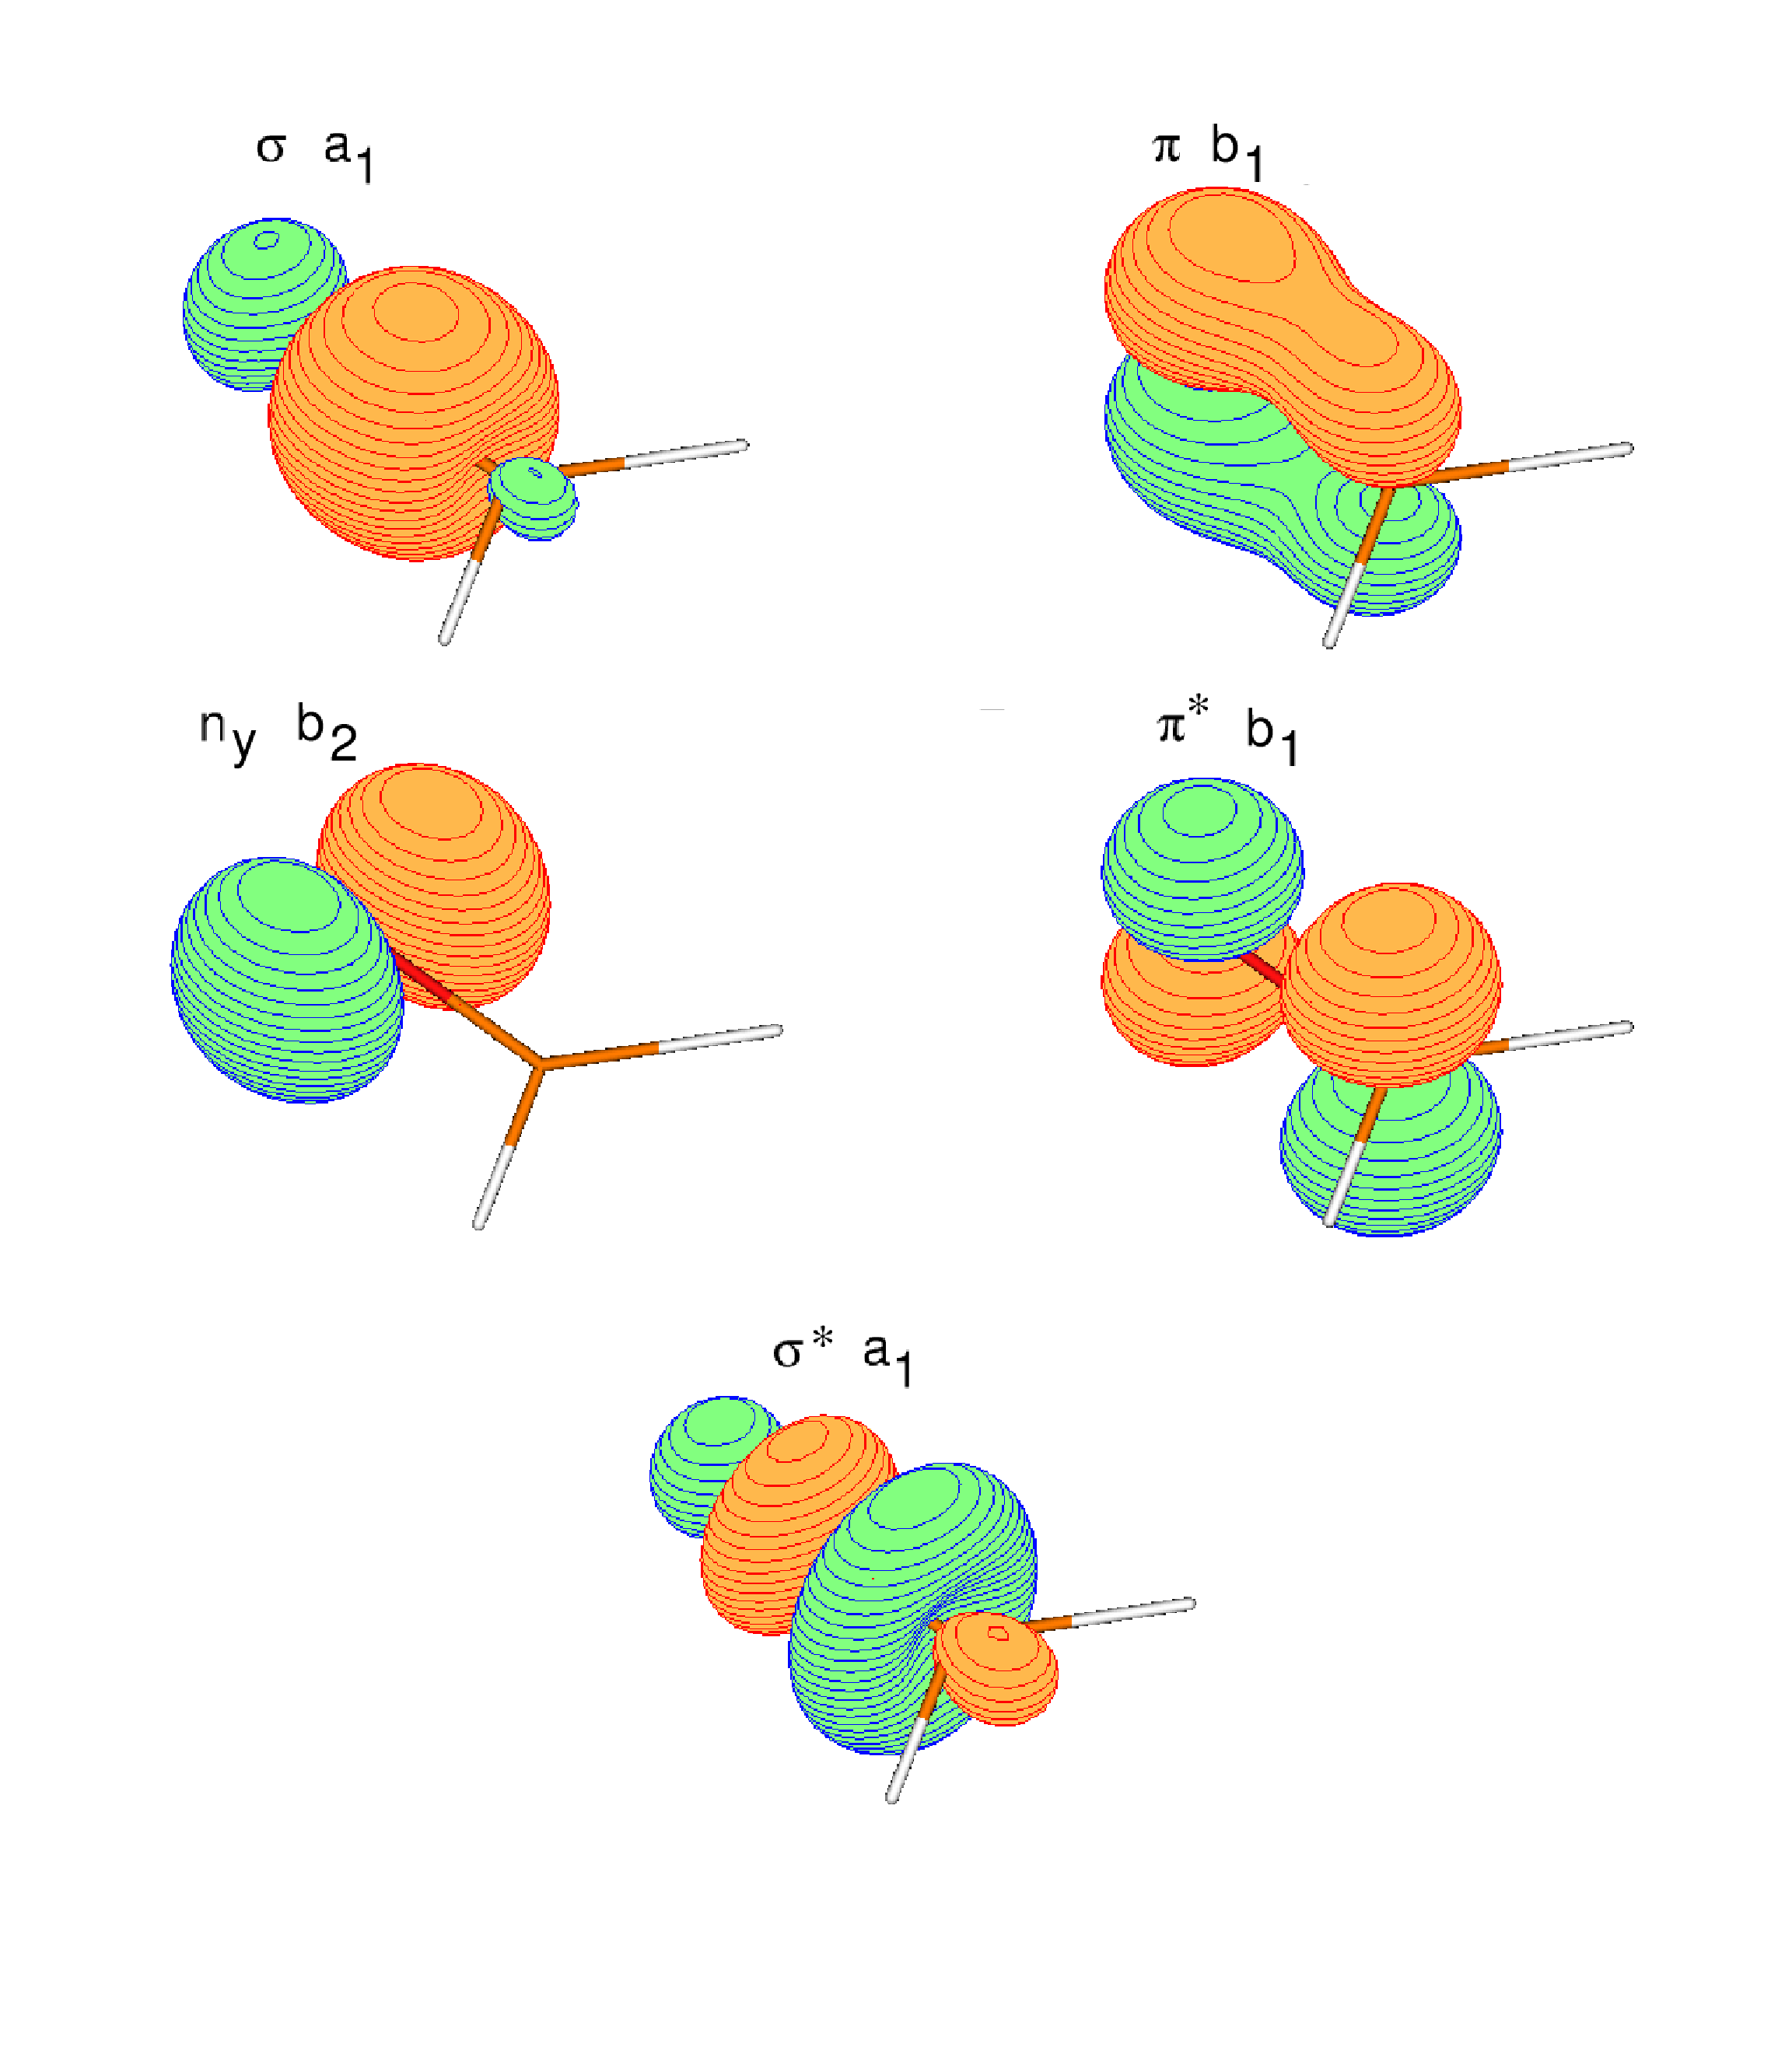
\includegraphics[width=8cm,keepaspectratio]{immagini/formaldeide/orbitali.eps}
\end{center}
\caption{Spazio CAS per la formaldeide}
\label{fig:formaldeide_orbitali}
\end{figure}

Nella trattazione HF gli orbitali doppiamente occupati sono
\begin{itemize}
\item 5 di simmetria A$_1$
\item 1 di simmetria B$_1$
\item 2 di simmetria B$_2$
\end{itemize}
Lo spazio CAS \`e stato costruito utilizzando, per lo spazio di core
(doppiamente occupato) 4 orbitali A$_1$ e 1 orbitale B$_2$,
mentre lo spazio attivo \`e stato definito da 2 orbitali A$_1$
(l'orbitale legante $\sigma$ e l'antilegante $\sigma^{*}$), 2 orbitali B$_1$
(un legante $\pi$ e l'antilegante $\pistar$) e 1 orbitale B$_2$ (non legante 
$n_y$), con 6 elettroni attivi e 10 elettroni di core.
Con questa scelta, sono necessarie 18 configurazioni per descrivere la molecola
nello stato fondamentale (simmetria A$_1$). 

Nel caso della transizione elettronica di interesse, si avr\`a la promozione
di un elettrone dall'orbitale $n_y$, di simmetria B$_2$, all'orbitale $\pistar$,
di simmetria B$_1$. La tabella dei prodotti diretti delle rappresentazioni
per il gruppo C$_{2v}$ 
\begin{center}
\begin{tabular}{|c|cccc|}
\hline
 C$_{2v}$ & A$_1$ & B$_1$ & B$_2$ & A$_2$ \\
\hline                                
    A$_1$ & A$_1$ &       &       &        \\
    B$_1$ & B$_1$ & A$_1$ &       &        \\
    B$_2$ & B$_2$ & A$_2$ & A$_1$ &        \\
    A$_2$ & A$_2$ & B$_2$ & B$_1$ & A$_1$  \\
\hline
\end{tabular}
\end{center}
indica per lo stato elettronico finale la simmetria B$_2 \otimes $B$_1 = $A$_2 $.

Il calcolo ha fornito, per lo spazio attivo del ground state, i seguenti numeri
di occupazione
\begin{verbatim}
 Simmetria A1 : 1.978929123   0.021519393
 Simmetria B1 : 1.929961079   0.070506119
 Simmetria B2 : 1.999084286
\end{verbatim}

L'energia CASSCF finale \`e -113.968732 Hartree, che si assume come energia
del ground state per il calcolo della transizione sulla base 6-311G*
a livello CASSCF.

%Limitatamente alla molecola di formaldeide sono state inoltre calcolate le
%energie di eccitazione per le transizioni $n_z \rightarrow \pistar$ e $\pi \rightarrow
%\pistar$, che comportano uno stato elettronico finale di simmetria $A_1 \otimes B_1 = B_1$
%e $B_1 \otimes B_1 = A_1$ rispettivamente. Di conseguenza, nel caso della
%transizione $\pi \rightarrow \pistar$, non avviene cambiamento di simmetria, dal momento
%che il ground state \`e anch'esso di simmetria $A_1$. L'energia dello stato eccitato
%sar\`a quindi la seconda radice della diagonalizzazione nella simmetria del ground state.

%In tabella \ref{tab:formaldeide_vertical} riportiamo i valori ottenuti per le varie transizioni,
%affiancate al dato sperimentale
%\begin{center}
%\begin{threeparttable}
%\caption{Formaldeide - energie di transizione verticale CAS/6-311G*}
%\label{tab:formaldeide_vertical}
%\small
%\begin{tabular}{|ccccc|}
%\hline
%							& Simm.		& Energia\tnote{1}	& Eccitato - GS\tnote{2} & Sperim.\tnote{2} \\
%\hline
%$GS$ 						& A1		& 1.96873 			& 0		& 0   \\
%$n_y \rightarrow \pistar$ 	& A2		& 1.80577 			& 4.43  & 4.07 \\
%$n_z \rightarrow \pistar$ 	& B1		& 1.59497			& 10.17 & 9.97 \tnote{3} \\
%$\pi \rightarrow \pistar$   & A1        & 1.55132           & 11.36 & 9.19 \tnote{3} \\
%\hline
%\end{tabular}
%\begin{tablenotes}
%\tiny
% \item[1] Energia come - (112 + valore) Hartree.
% \item[2] Valore in eV
% \item[3] Valore sperimentale non disponibile. Dati da CIS-MP2 su 6-311(2+,2+)G** (Cfr. \cite{jpc-97-17-1993-4293})
%\end{tablenotes}
%\end{threeparttable}
%\end{center}

Il calcolo effettuato sullo stato eccitato di simmetria A$_2$, mantenendo la
geometria ottimizzata per lo stato fondamentale (transizione verticale) ha fornito
invece un'energia di -113.80577 Hartree, comportando di conseguenza un'energia di
transizione elettronica pari a 4.43 eV, che confrontato al valore sperimentale
4.07 eV (Cfr. \cite{jpc-99-20-1995-8050}) evidenzia un errore di circa 0.4 eV. 
%Le altre transizioni non sono esattamente
%definite, e non vi sono ancora riferimenti bibliografici certi sull'assegnazione energetica
%della transizione $\pi \rightarrow \pistar$, che dovrebbe giacere tra i 9 e gli 11 eV. (Cfr.
%\cite{jpc-99-20-1995-8050}). Per questa ragione, tali calcoli non verranno affrontati su molecole
%pi\`u complesse, ma limiteremo il nostro studio alla sola transizione verticale e adiabatica
%$n_y \rightarrow \pistar$.

I numeri di occupazione confermano la transizione $n_y \rightarrow \pistar$
\begin{verbatim}
 Simmetria A1 : 1.984641659   0.015707156
 Simmetria B1 : 1.996255549   1.003395636
 Simmetria B2 : 1.000000000
\end{verbatim}

\`E stata successivamente condotta un'ottimizzazione di geometria per lo
stato eccitato, valutando di conseguenza la transizione adiabatica. In tali
condizioni, la simmetria del sistema cala da C$_{2v}$ a C$_s$, venendo a
mancare un piano di riflessione in seguito alla piramidalizzazione della
molecola.

\begin{center}
\begin{threeparttable}
\caption{\small Formaldeide - geometrie di transizione adiabatica}
\label{tab:formaldeide_geometrie_adiab}
\begin{tabular}{|c|cc|}
\hline
					& GS		& $n_y \rightarrow \pistar$ \\ %& $n_z \rightarrow \pistar$	\\
\hline
$r$(C-O)		 	& 1.2161	&  1.3817 				\\ %& 1.541100 					 \\
$r$(C-H)			& 1.0885	&  1.0762					\\ %& 1.078499					 \\
$\angle$(H-C-H)		& 117.20	&  119.44					\\ %& 115.812					 \\
$\angle$(H-C-O)		& 121.40	&  113.03					\\ %& 110.473					 \\
Energia 			& 1.968732	&  1.834522					\\ %& 1.673067					 \\
En. Eccitazione 	& 			&  3.65						\\ %& 8.04						 \\
En. Ecc. Exp.\tnote{1} & 	&  3.50						\\ %& 8.49						 \\
\hline
\end{tabular}
\begin{tablenotes}
\small
 \item[1] Cfr. \cite{sa-34a-1978-749} e \cite{jpc-97-17-1993-4293}
 \item[] Valori in Angstroms, angoli in gradi, Energie assolute come
  \mbox{-(112 + valore)} Hartree, energie di eccitazione in eV
\end{tablenotes}
\end{threeparttable}
\end{center}

La geometria da planare muta in piramidale. \`E osservabile uno spostamento
degli atomi di idrogeno fuori dal piano molecolare ed un allungamento del
legame C-O dovuto all'occupazione di un orbitale di antilegame $\pistar$,
accompagnato da una netta diminuzione dell'angolo di legame H-C-O verso
valori caratteristici di una geometria piramidale.

A causa del calo di simmetria del sistema, gli orbitali precedentemente
riconducibili alle rappresentazioni A$_1$ e B$_1$ appartengono ora alla
rappresentazione A$^{\prime}$, mentre gli orbitali appartenenti alle 
rappresentazioni B$_2$ e A$_2$ ora saranno di simmetria A$^{\prime\prime}$.
Lo spazio attivo precedentemente definito vedr\`a di conseguenza, 
$\sigma$, $\sigma^{*}$, $\pi$ e $\pistar$ appartenere ad A$^{\prime}$,
e $n_y$ ad A$^{\prime\prime}$. Una transizione elettronica $n_y \rightarrow
\pistar$ avr\`a simmetria A$^{\prime\prime} \otimes $A$^{\prime} =
$A$^{\prime\prime}$

Lo stato eccitato ha un'energia CASSCF pari a -113.834522
Hartree, che comporta un'energia di transizione di 3.65 eV, contro un valore
sperimentale di 3.50 eV (Cfr. \cite{jpc-97-17-1993-4293} e \cite{sa-34a-1978-749})

\subsubsection{Dipendenza dalla base atomica}

Per valutare la dipendenza dalla base atomica utilizzata si sono effettuati calcoli per
le transizioni verticale e adiabatica $ n_y \rightarrow \pistar $ su differenti 
set di base, in ordine di dimensionalit\`a:
\begin{itemize}
 \item 6-31G (Cfr. \cite{mp-27-1974-209})
 \item cc-pVDZ (Cfr. \cite{jcp-90-1989-1007})
 \item ano-1 (Cfr. \cite{jcp-55-1971-4798}) con riduzione 3s2p1d per il carbonio e 2s1p per l'idrogeno
 \item 6-311G* (Cfr. \cite{jcp-72-1980-5639})
 \item cc-pVTZ (Cfr. \cite{jcp-90-1989-1007})
 \item cc-pVQZ (Cfr. \cite{jcp-90-1989-1007})
\end{itemize}
Su ogni base \`e stata effettuata una ottimizzazione di geometria della
molecola, a livello CASSCF.

La tabella \ref{tab:formaldeide_vertical_basis} riporta i risultati ottenuti
per la transizione verticale. \`E evidente come basi a dimensionalit\`a molto
elevata, come cc-pVTZ e cc-pVQZ, portino a risultati pressoch\'e identici.
\`E quindi prevedibile che una ulteriore estensione della base non fornirebbe
risultati pi\`u accurati di quelli ottenuti, e comporterebbe un notevole incremento
dei tempi di calcolo. L'errore commesso a livello CASSCF resta
considerevole, essendo di 0.34 eV.  Una possibile soluzione alternativa \`e
ricercabile nell'allargamento dello spazio CAS, che aumenterebbe in modo
deciso la complessit\`a computazionale.

Di conseguenza, per cercare di migliorare i risultati CASSCF abbiamo
condotto dei calcoli perturbativi utilizzando la teoria NEV-PT, ottenendo
ottimi risultati con tempi di calcolo pi\`u che accettabili. La
tabella \ref{tab:formaldeide_vertical_basis} mostra quanto ottenuto, sia per
l'approccio Strongly Contracted (NEV-PT/SC) che per quello Partially Contracted
(NEV-PT/PC).

\begin{center}
\begin{threeparttable}
\caption{\small Formaldeide - Energia di transizione $n_y \rightarrow \pistar$ verticale di singoletto, metodi CASSCF e CASSCF/NEV-PT}
\label{tab:formaldeide_vertical_basis}
{
\small
\begin{tabular}{|c|ccc|ccc|}
\hline
 Base	& \multicolumn{3}{c}{GS\tnote{1}}				& \multicolumn{3}{c|}{$n_y \rightarrow \pistar$ vert.\tnote{2}} \\
		& CASSCF		& NEV-PT & NEV-PT	& CASSCF		& NEV-PT & NEV-PT \\
		& 				& SC	 & PC		& 				& SC 	& PC \\
\hline
6-31G	& 1.891188		& 2.019821		& 2.021959		& 3.85			& 3.73		& 3.72		    \\
cc-pVDZ	& 1.950044		& 2.183100		& 2.185533		& 4.38			& 4.07 		& 4.10			\\
ano-1	& 1.978883		& 2.207808		& 2.210750		& 4.36			& 4.02 		& 4.01			\\
6-311G*	& 1.968732		& 2.242321		& 2.244788		& 4.43 			& 4.07		& 4.11 			\\
cc-pVTZ & 1.985284 		& 2.316323		& 2.319135		& 4.40			& 4.04 		& 4.02			\\
cc-pVQZ & 1.994326		& 2.381916		& 2.384828		& 4.41			& 4.04		& 4.02			\\
\hline
\hline
Exp.	&				& 				&				& \multicolumn{3}{c|}{4.07} \\
\hline
\end{tabular}
}
\begin{tablenotes}
\small
 \item[1] Energia come -(112 + valore) Hartree
 \item[2] Valori in eV
\end{tablenotes}
\end{threeparttable}
\end{center}

Per quanto riguarda la transizione adiabatica, si \`e tenuto conto della differenza
tra le energie di punto zero (Zero Point Energy, ZPE) dei due stati elettronici. Questa differenza deriva
dalla diversa struttura della superficie di potenziale per lo stato fondamentale ed
eccitato, che si riflette in una diversa energia dello stato vibrazionale
fondamentale per i due stati elettronici. Assumendo che l'effetto perturbativo non attui modifiche
significative sulla struttura del potenziale CASSCF, ma si limiti ad una
traslazione energetica omogenea, le energie di punto zero per i calcoli
perturbativi possono essere assunte uguali a quella CASSCF. 
Ci\`o non \`e strettamente garantito, tuttavia \`e una approssimazione necessaria,
in quanto una accurata valutazione di questo effetto necessiterebbe di un
calcolo accurato di tutta la superficie di potenziale a livello
perturbativo.
Per questa ragione, la correzione ZPE
\`e stata applicata allo stesso modo sia sul calcolo CASSCF che sul calcolo 
perturbativo.

\begin{center}
\begin{threeparttable}
\caption{\small Formaldeide - Energia di transizione $n_y \rightarrow \pistar$ adiabatica di singoletto, calcolata a livello CASSCF e NEV-PT}
\label{tab:formaldeide_basis_energy}
{
\small
\begin{tabular}{|c|cccccc|}
\hline
Base	& ZPE 			& ZPE 				& $\Delta$ZPE	& CASSCF	& NEV-PT	& NEV-PT \\
		& (GS)			& (Ecc.)			& 				& ZPE 		&   SC/ZPE 	& PC/ZPE \\
\hline
6-31G	& 0.766			& 0.685				& -0.081		&  3.13		& 3.12			  & 3.14			\\
cc-pVDZ & 0.760			& 0.692				& -0.068        &  3.56		& 3.49			  & 3.50			\\
ano-1	& 0.764			& 0.696				& -0.068		&  3.55		& 3.43			  & 3.45			\\
6-311G* & 0.765			& 0.700				& -0.066		&  3.59		& 3.52			  & 3.57			\\
cc-pVTZ & 0.759         & 0.692				& -0.067		&  3.60		& 3.55			  & 3.56			\\
cc-pVQZ & 0.760			& 0.693				& -0.067		&  3.61		& 3.58			  & 3.59			\\
\hline
\hline
Exp.	&				& 					& 				& \multicolumn{3}{c|}{3.50}						\\
\hline
\end{tabular}
}
\begin{tablenotes}
\small
 \item[ ] Valori in eV
\end{tablenotes}
\end{threeparttable}
\end{center}

In figura \ref{fig:formaldeide_gs} sono rappresentate le energie elettroniche del
ground state a livello CASSCF (linea rossa), NEV-PT/SC (linea verde) e
NEV-PT/PC (linea blu), in funzione della base atomica scelta, in ordine di
dimensionalit\`a. Come si pu\`o notare, la NEV-PT/SC fornisce
risultati di pochissimo superiori in energia alla NEV-PT/PC.

\begin{figure}[ht]
\begin{center}
\includegraphics[angle=270,width=10cm,keepaspectratio]{immagini/formaldeide/gs.eps}
\parbox[h]{10cm}{
\caption{\small Formaldeide - Energia dello stato fondamentale a livello CASSCF (linea rossa),
NEV-PT/SC (linea verde) e NEV-PT/PC (linea blu). }
\label{fig:formaldeide_gs}
}
\end{center}
\end{figure}
\clearpage

Analogamente, le figure \ref{fig:formaldeide_vert} e
\ref{fig:formaldeide_adiab} forniscono la medesima rappresentazione
relativamente agli stati eccitati calcolati alla geometria di equilibrio
dello stato fondamentale e dello stato eccitato rispettivamente. 

\begin{figure}[ht]
\begin{center}
\includegraphics[angle=270,width=7cm,keepaspectratio]{immagini/formaldeide/vert.eps}
\parbox[h]{12cm}{
\caption{\small Formaldeide - Energia dello stato eccitato (transizione verticale)
a livello CASSCF (linea rossa), NEV-PT/SC (linea verde) e NEV-PT/PC (linea blu) come
funzione della base atomica. }
\label{fig:formaldeide_vert}
}
\end{center}
\end{figure}
\begin{figure}[ht]
\begin{center}
\includegraphics[angle=270,width=7cm,keepaspectratio]{immagini/formaldeide/adiab.eps}
\parbox[h]{12cm}{
\caption{\small Formaldeide - Energia dello stato eccitato (transizione
adiabatica) a livello CASSCF (linea rossa), NEV-PT/SC (linea verde) e NEV-PT/PC (linea blu) come
funzione della base atomica. }
\label{fig:formaldeide_adiab}
}
\end{center}
\end{figure}
\clearpage

Diagrammando l'energia della transizione verticale contro la base, si ottiene
il grafico in figura \ref{fig:formaldeide_energie_vert}. La simbologia
utilizzata \`e analoga a quella della figura precedente. La linea viola denota
il valore sperimentale di $4.07$ eV.

\begin{figure}[ht]
\begin{center}
\includegraphics[angle=270,width=12cm,keepaspectratio]{immagini/formaldeide/energie_vert.eps}
\parbox[h]{12cm}{
\caption{\small Formaldeide - energia di transizione verticale su basi differenti a livello CASSCF (linea rossa), NEV-PT/SC (linea verde) e NEV-PT/PC (linea blu) come funzione della base atomica.}
\label{fig:formaldeide_energie_vert}
}
\end{center}
\end{figure}

\`E possibile vedere come la transizione verticale venga descritta con buona accuratezza
anche con basi piccole, una volta che si sia introdotta la correzione perturbativa.
\clearpage

L'energia della transizione adiabatica in figura
\ref{fig:formaldeide_energie_adiab} mostra invece l'andamento di tale
parametro contro il valore sperimentale di $3.50$ eV.

\begin{figure}[ht]
\begin{center}
\includegraphics[angle=270,width=12cm,keepaspectratio]{immagini/formaldeide/energie_adiab.eps}
\parbox[h]{12cm}{
\caption{\small Formaldeide - energia di transizione adiabatica su basi differenti a livello CASSCF (linea rossa), NEV-PT/SC (linea verde) e NEV-PT/PC (linea blu) come funzione della base atomica.}
\label{fig:formaldeide_energie_adiab}
}
\end{center}
\end{figure}

\clearpage

%%%%%%%%%%%%%%%%%%%%%%%%%%%%%%%%%%%%%%%%%%%%%%%

\subsection{Acetone}

Analoga trattazione \`e stata effettuata nel caso della molecola di acetone.
La geometria iniziale, fornita attraverso z-matrix, possiede configurazione C$_{2v}$,
con gli atomi di idrogeno metilici sul piano, non affacciati.

\begin{figure}[ht]
\begin{center}
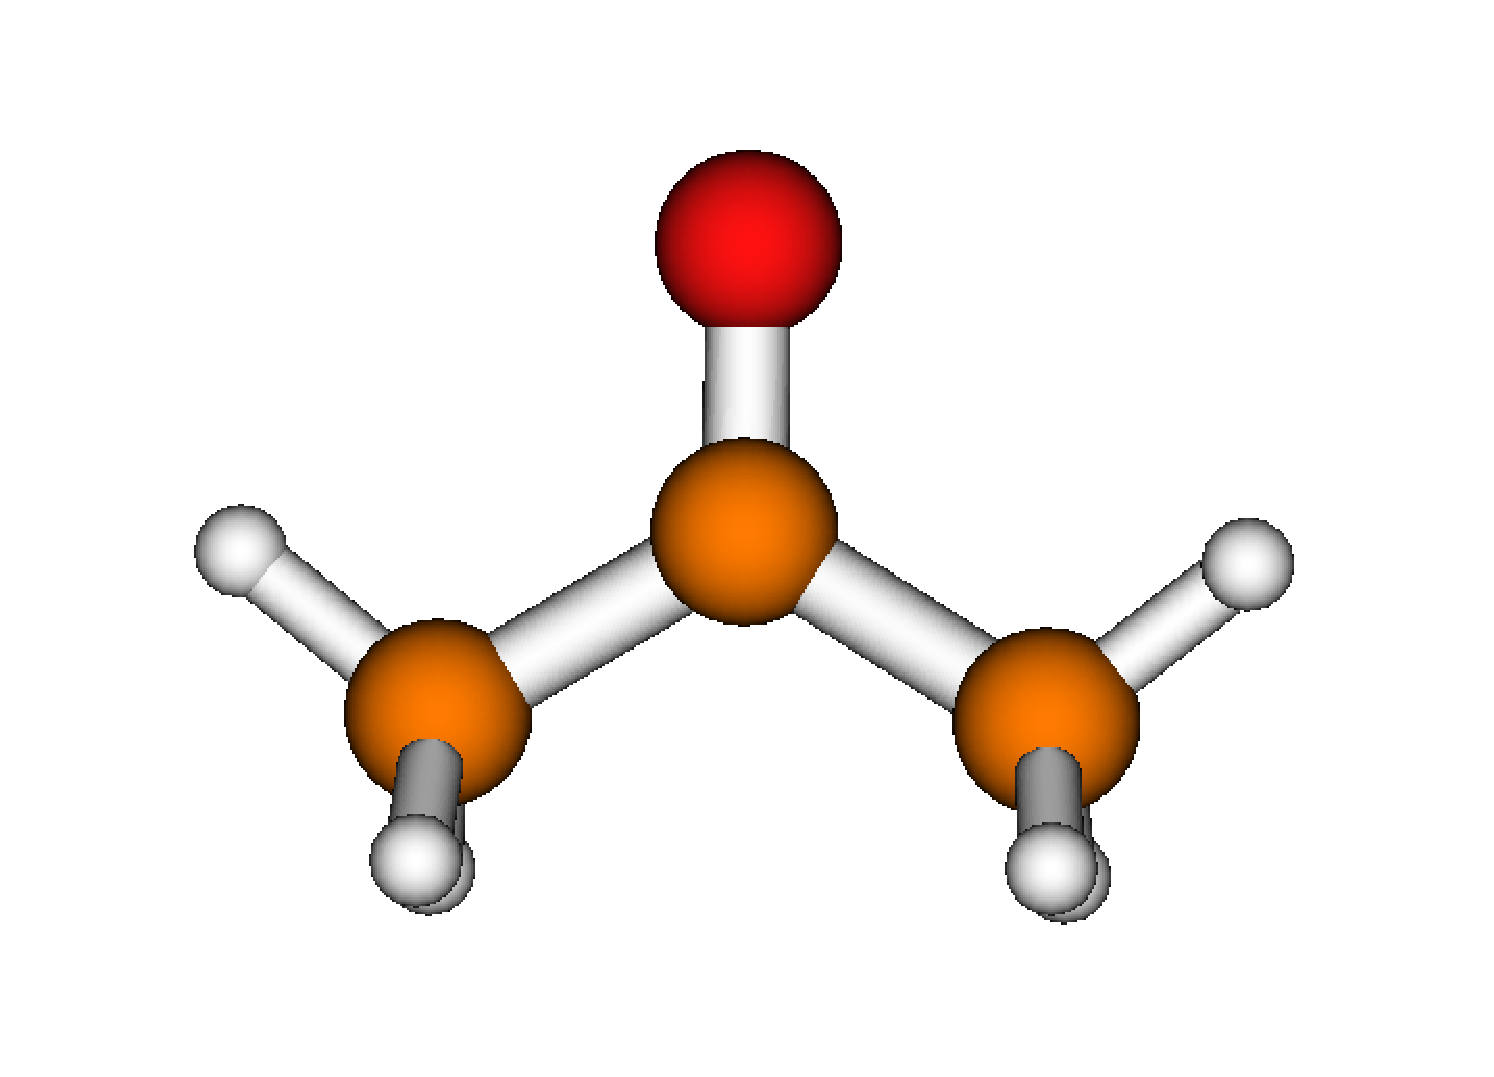
\includegraphics[angle=270,width=7cm,keepaspectratio]{immagini/acetone/geom.eps}
\parbox[h]{12cm}{
\caption{\small Acetone - configurazione spaziale per lo stato fondamentale}
\label{fig:acetone_geom}
}
\end{center}
\end{figure}

L'ottimizzazione di geometria \`e stata effettuata con base 6-311G* a livello CAS,
con uno spazio analogo a quello della formaldeide. La tabella \ref{tab:acetone_geom}
mette a confronto alcuni risultati con il dato sperimentale.
\begin{center}
\begin{threeparttable}
\caption{Acetone - geometria stato fondamentale}
\label{tab:acetone_geom}
\small
\begin{tabular}{|ccc|c|}
\hline
							& CASSCF	& Exp.\tnote{1} \\ 
\hline
$r$(C-O)\tnote{2}			& 1.221		& 1.222				\\
$r$(C-C)\tnote{2}			& 1.511		& 1.507				 \\
$r$(C-H$_1$)\tnote{3}			& 1.081		&			 		 \\
$r$(C-H$_2$)\tnote{3}			& 1.086		&				 	 \\
$\angle$(O-C-C)				& 121.33	& 121.49			 \\
$\angle$(C-C-C)				& 117.33	& 117.02			 \\
\hline
\end{tabular}
\begin{tablenotes}
\parbox[h]{6cm}{
\small
 \item[1] Cfr. \cite{jms-550-551-2000-281}, \cite{jms-120-1986-118} e
 \cite{mp-31-1976-1377}
 \item[] Distanze in Angstroms, angoli in gradi. H$_1$ fa riferimento agli
         idrogeni coplanari al carbonile. H$_2$ agli idrogeni sopra e sotto tale
         piano
}
\end{tablenotes}
\end{threeparttable}
\end{center}
Come si pu\`o notare, la distanza C=O aumenta leggermente, se confrontata
con quella della formaldeide di 1.216 \AA. Ci\`o \`e interpretabile in seguito
all'aumento di interazione sterica tra la nuvola di carica del carbonile e i
gruppi metilici.

La trattazione MCSCF ha richiesto
18 configurazioni, per uno spazio di 6 elettroni in 5 orbitali, illustrati
in figura \ref{fig:acetone_orbitali}. Dal momento che l'acetone possiede la
medesima simmetria della formaldeide, le rappresentazioni irriducibili a cui
apparterranno gli orbitali saranno le medesime elencate in precedenza: A$_1$, B$_1$,
B$_2$ e A$_2$. La distribuzione HF per la molecola di acetone sar\`a quindi
\begin{itemize}
\item 8 di simmetria A$_1$
\item 2 di simmetria B$_1$
\item 5 di simmetria B$_2$
\item 1 di simmetria A$_2$
\end{itemize}

Data la scelta dello spazio CAS, lo spazio inattivo risulta essere
costituito da 7 orbitali di simmetria A$_1$, 1 orbitale di simmetria B$_1$,
4 orbitali di simmetria B$_2$ e 1 orbitale di simmetria A$_2$. Analogamente
al caso della formaldeide, lo stato elettronico finale della transizione
$n_y \rightarrow \pistar$ sar\`a B$_2 \otimes $B$_1 = $A$_2 $.

\begin{figure}[htb]
\begin{center}
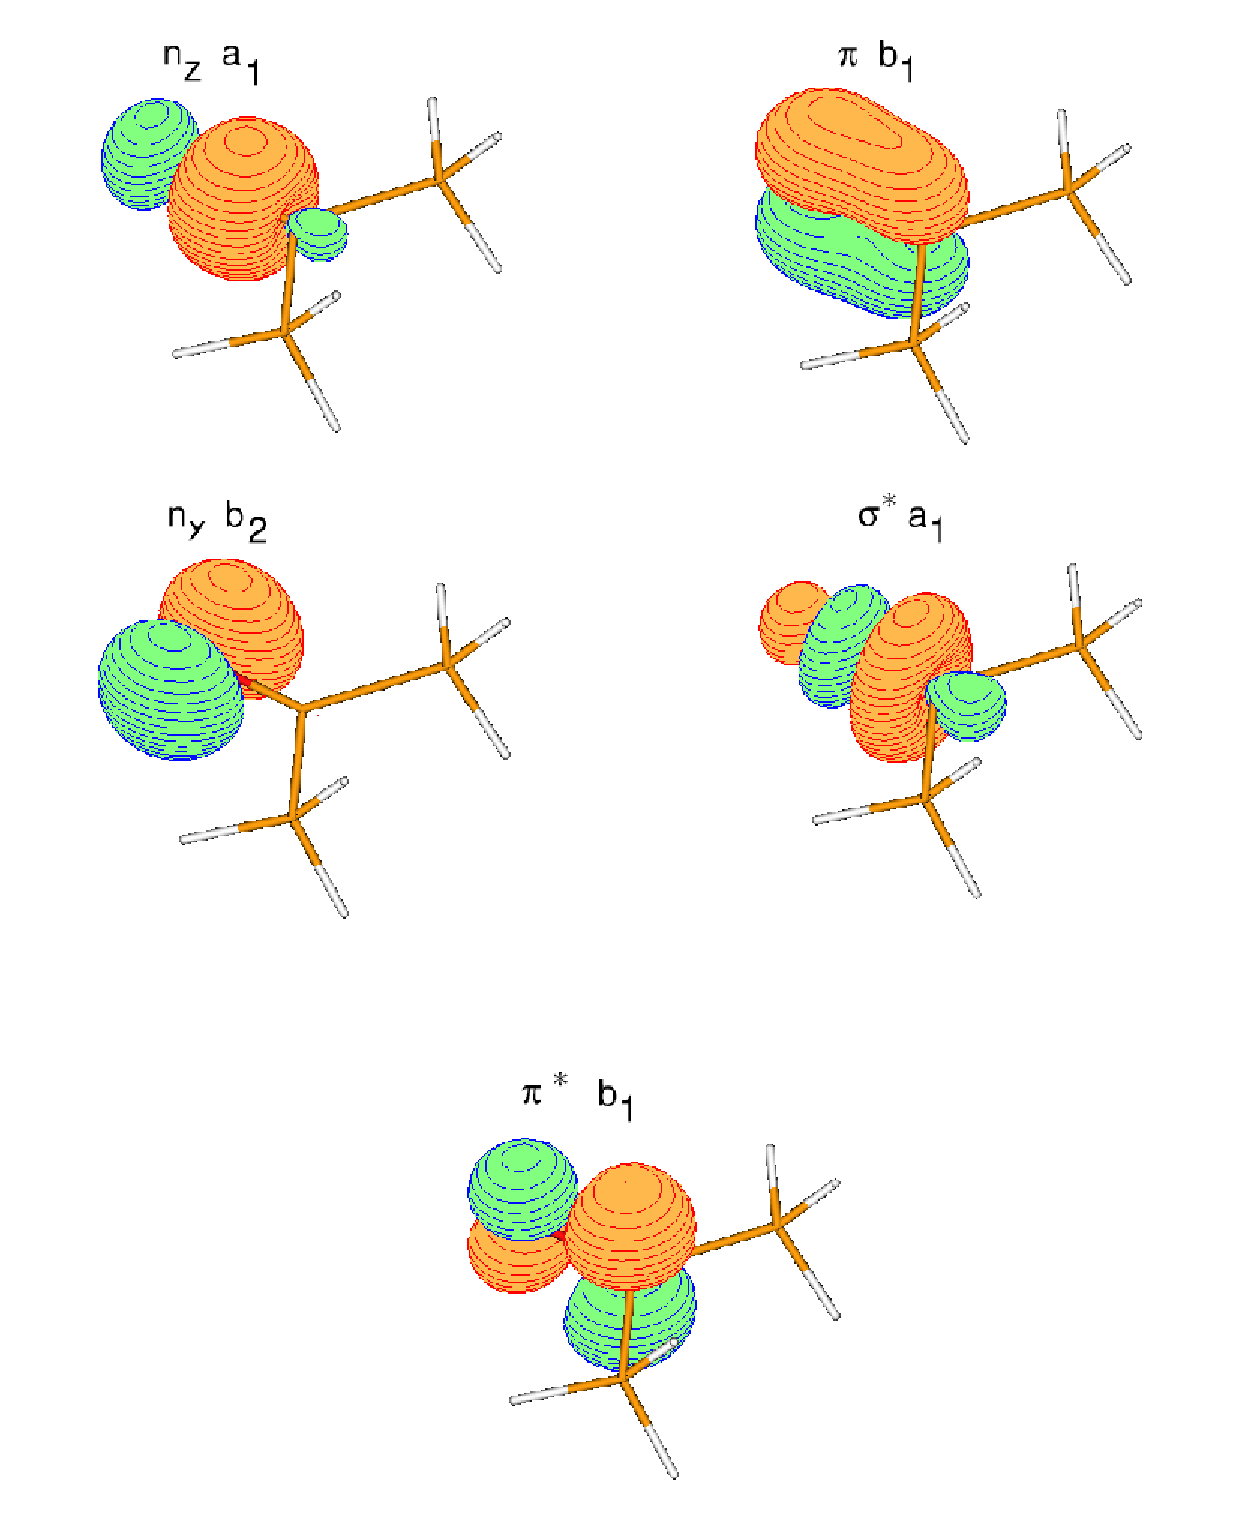
\includegraphics[width=8cm,keepaspectratio]{immagini/acetone/orbitali.eps}
\end{center}
\caption{Spazio CAS per l'acetone}
\label{fig:acetone_orbitali}
\end{figure}

La tabella mostra i numeri di occupazione per lo
stato fondamentale
\begin{verbatim}
 Simmetria A1 : 1.978732113   0.021697330
 Simmetria B1 : 1.938253072   0.062093260 
 Simmetria B2 : 1.999224225
\end{verbatim}

L'energia CASSCF finale per questa base (6-311G*) \`e -192.074240 Hartree.

L'analisi della transizione verticale ha fornito, per lo stato eccitato, un'energia 
-191.895199 Hartree, con una transizione rispetto allo stato fondamentale
di 4.87 eV, contro un valore sperimentale di 4.43 eV (Cfr. \cite{cpl-241-0-1995-26}).
La tabella seguente mostra i numeri di occupazione per lo
stato eccitato
\begin{verbatim}
 Simmetria A1 : 1.984561941   0.015780241 
 Simmetria B1 : 1.996558895   1.003098923
 Simmetria B2 : 1.000000000
\end{verbatim}

Il calcolo effettuato per la transizione adiabatica ha fornito un'energia finale di
-191.932347 Hartree, pari ad una transizione di 3.86 eV contro un valore sperimentale di 3.77 eV
(Cfr. \cite{jcp-111-1-1999-205}). Anche in questo caso, come \`e prevedibile,
il legame carbonilico si allunga in seguito all'occupazione dell'orbitale di
antilegame.
\begin{center}
\begin{threeparttable}
\caption{\small Acetone - geometria di transizione adiabatica}
\label{tab:acetone_geometrie_adiab}
\small
\begin{tabular}{|c|cc|}
\hline
				& CASSCF	& $n_y \rightarrow \pistar$  \\
\hline
$r$(C-O)			& 1.221		& 1.397				\\
$r$(C-C)		& 1.511		& 1.499				 \\
$r$(C-H$_1$)		& 1.080		& 1.084		 		 \\
$r$(C-H$_2$)		& 1.086		& 1.083			 	 \\
$r$(C-H$_3$)		& 1.086		& 1.089			 	 \\
$\angle$(O-C-C)		& 121.33	& 112.13			 \\
$\angle$(C-C-C)		& 117.33	& 121.32			 \\
\hline
\end{tabular}
\begin{tablenotes}
\small
 \item[] Distanze in Angstroms, angoli in gradi
\end{tablenotes}
\end{threeparttable}
\end{center}

\subsubsection{Dipendenza dalla base atomica}

Similmente alla molecola di formaldeide, abbiamo condotto calcoli a
livello CASSCF e perturbativo con le basi
\begin{itemize}
 \item 6-31G
 \item cc-pVDZ
 \item ano-1 (con riduzione 3s2p1d per il carbonio e 2s1p per l'idrogeno)
 \item 6-311G* 
 \item cc-pVTZ
 \item cc-pVQZ
\end{itemize}
i risultati sono mostrati in tabella \ref{tab:acetone_vertical_basis}
\begin{center}
\begin{threeparttable}
\caption{\small Acetone - Energia di transizione $n_y \rightarrow \pistar$ verticale di singoletto, metodi CASSCF e CASSCF/NEV-PT}
\label{tab:acetone_vertical_basis}
{
\small
\begin{tabular}{|c|ccc|ccc|}
\hline
 Base	& \multicolumn{3}{c|}{GS\tnote{1}}				& \multicolumn{3}{c|}{$n_y \rightarrow \pistar$ vert.\tnote{2}} \\
		& CASSCF		& NEV-PT	& NEV-PT	& CASSCF		& NEV-PT & NEV-PT \\
		& 				& SC		& PC		&				& SC 	&	 PC \\
\hline
6-31G	& 0.953869		& 1.263394		& 1.265603		& 4.31			& 4.19		& 4.19		    \\
cc-pVDZ	& 1.048077		& 1.567089		& 1.569608		& 4.84			& 4.50		& 4.50			\\
ano-1	& 1.095777		& 1.612795		& 1.615686 		& 4.87			& 4.54 		& 4.53			\\
6-311G*	& 1.074240		& 1.658429		& 1.660956		& 4.87 			& 4.53		& 4.54 			\\
cc-pVTZ & 1.104413		& 1.810794		& 1.813551		& 4.90			& 4.51 		& 4.51			\\
\hline
\hline
Exp.\tnote{3}	&				& 				&				& \multicolumn{3}{c|}{4.43} \\
\hline
\end{tabular}
}
\begin{tablenotes}
\small
 \item[1] Energia come -(191 + valore) Hartree.
 \item[2] Valori in eV.
 \item[3] Cfr. \cite{cpl-241-0-1995-26}
\end{tablenotes}
\end{threeparttable}
\end{center}

Per quanto riguarda la transizione adiabatica, in tabella \ref{tab:acetone_adiab_basis},
si \`e nuovamente tenuto conto della differenza di ZPE tra lo stato fondamentale e quello eccitato.

\begin{center}
\begin{threeparttable}
\caption{\small Acetone - Energia di transizione $n_y \rightarrow \pistar$ adiabatica di singoletto, metodi CASSCF e CASSCF/NEV-PT}
\label{tab:acetone_adiab_basis}
{
\small
\begin{tabular}{|c|ccc|ccc|}
\hline
Base	& ZPE		& ZPE 			& $\Delta$ZPE	& CASSCF & NEV-PT & NEV-PT \\
		& (GS)		& (Ecc.)		& 				& ZPE 	& SC/ZPE & PC/ZPE \\
\hline
6-31G	& 2.437			& 2.382				& -0.055		&  3.40		 & 3.36 		  & 3.38		\\
cc-pVDZ & 2.402			& 2.350				& -0.052		&  3.81		 & 3.70			  & 3.72		\\
ano-1	& 2.419 		& 2.369				& -0.050		&  3.81 	 & 3.69		  	  & 3.70		\\
6-311G* & 2.414			& 2.367				& -0.047		&  3.81		 & 3.72			  & 3.75		\\
cc-pVTZ & 2.399         & 2.350				& -0.049		&  3.84		 & 3.78		 	  & 3.80		\\
\hline
\hline
Exp.\tnote{1} &				& 					& 				& \multicolumn{3}{c|}{3.77}					\\
\hline
\end{tabular}
}
\begin{tablenotes}
\small
 \item[1] Cfr. \cite{jcp-111-1-1999-205}
 \item[] Valori in eV
\end{tablenotes}
\end{threeparttable}
\end{center}

Nelle figure \ref{fig:acetone_gs}, \ref{fig:acetone_vert} e
\ref{fig:acetone_adiab} sono diagrammate le energie assolute degli stati
fondamentale, eccitato verticale ed eccitato adiabatico rispettivamente,
a livello CASSCF (linea rossa), NEV-PT/SC (linea verde) e NEV-PT/PC
(linea blu).
\begin{figure}[ht]
\begin{center}
\includegraphics[angle=270,width=10cm,keepaspectratio]{immagini/acetone/gs.eps}
\parbox[h]{12cm}{
\caption{\small Acetone - Energia dello stato fondamentale a livello CASSCF (linea rossa),
NEV-PT/SC (linea verde) e NEV-PT/PC (linea blu) come funzione della base
atomica.}
\label{fig:acetone_gs}
}
\end{center}
\end{figure}
\begin{figure}[ht]
\begin{center}
\includegraphics[angle=270,width=10cm,keepaspectratio]{immagini/acetone/vert.eps}
\parbox[h]{12cm}{
\caption{\small Acetone - Energia dello stato eccitato (transizione verticale)
a livello CASSCF (linea rossa), NEV-PT/SC (linea verde) e NEV-PT/PC (linea blu)
come funzione della base atomica. }
\label{fig:acetone_vert}
}
\end{center}
\end{figure}
\begin{figure}[ht]
\begin{center}
\includegraphics[angle=270,width=10cm,keepaspectratio]{immagini/acetone/adiab.eps}
\parbox[h]{12cm}{
\caption{\small Acetone - Energia dello stato eccitato (transizione adiabatica)
a livello CASSCF (linea rossa), NEV-PT/SC (linea verde) e NEV-PT/PC (linea blu)
come funzione della base atomica. }
\label{fig:acetone_adiab}
}
\end{center}
\end{figure}
\pagebreak
\clearpage
Graficando l'energia delle transizioni verticale e adiabatica possiamo notare come
la trattazione perturbativa porti a migliori risultati anche in questo caso.
\begin{figure}[ht]
\begin{center}
\includegraphics[angle=270,width=9cm,keepaspectratio]{immagini/acetone/energie_vert.eps} \\
\includegraphics[angle=270,width=9cm,keepaspectratio]{immagini/acetone/energie_adiab.eps}
\parbox[h]{12cm}{
\caption{\small Acetone - energia di transizione verticale (in alto) e adiabatica (sopra) su basi differenti a livello CASSCF (linea rossa), NEV-PT/SC (linea verde) e NEV-PT/PC (linea blu) come funzione della base atomica.}
\label{fig:acetone_energie_vert_adiab}
}
\end{center}
\end{figure}
\clearpage
%\begin{figure}[ht]
%\begin{center}
%\includegraphics[angle=270,width=6cm,keepaspectratio]{immagini/acetone/energie_adiab.eps}
%\parbox[h]{12cm}{
%\caption{\small Acetone - energia di transizione adiabatica su basi differenti a livello CASSCF (linea rossa), NEV-PT/SC (linea verde) e NEV-PT/PC (linea blu) come funzione della base atomica.}
%\label{fig:acetone_energie_adiab}
%}
%\end{center}
%\end{figure}
%\clearpage

\subsection{Acetaldeide}

Abbiamo successivamente analizzato la molecola di acetaldeide
\begin{figure}[ht]
\begin{center}
\includegraphics[angle=270,width=7cm,keepaspectratio]{immagini/acetaldeide/geom.eps}
\parbox[h]{10cm}{
\caption{\small Acetaldeide - configurazione spaziale per lo stato fondamentale}
\label{fig:acetaldeide_geom}
}
\end{center}
\end{figure}

Appartenente al gruppo C$_s$, l'acetaldeide ha presentato maggiori
difficolt\`a durante la trattazione richiesta, a causa della ridotta
simmetria rispetto alle molecole precedentemente analizzate. Tale
diversit\`a non consente un perfetto controllo della natura degli orbitali
che definiscono lo spazio CAS: la
selezione degli orbitali gi\`a descritta in precedenza deve ora appartenere
a due sole rappresentazioni irriducibili, la A$^{\prime}$ e la A$^{\prime\prime}$.

Nella tabella dei caratteri qui sotto riportata abbiamo posto l'asse $z$
allineato con il gruppo carbonile, ed il piano $yz$ come elemento di
simmetria per la riflessione \begin{center}
\begin{tabular}{c|cc|c}
  C$_s$				& E		& $\sigma_{yz}$	&           \\
\hline
    A$^{\prime}$  		& 1		&   1			&  $y$, $z$	\\
    A$^{\prime\prime}$	& 1		&  -1			&  $x$      \\
\end{tabular}
\end{center}
In questo modo, \`e possibile interpretare la molecola di acetaldeide, dal
punto di vista della simmetria, in maniera analoga alle molecole viste in
precedenza. Per questa ragione, gli orbitali $\pi$ e $\pistar$ apparterranno alla
rappresentazione irriducibile A$^{\prime\prime}$, in quanto antisimmetrici
rispetto alla riflessione sul piano della molecola, mentre i restanti
orbitali $n_y$, $\sigma$ e $\sigma^{*}$ apparterranno alla rappresentazione
A$^{\prime}$.

Al solito, si \`e scelto uno spazio attivo compatibile alle precedenti
caratterizzazioni e si sono effettuati calcoli sulla base 6-311G* al fine di
ottenere la geometria dello stato fondamentale. 
La scelta ha comportato uno spazio inattivo costituito da 8 orbitali di
simmetria A$^{\prime}$ e 1 orbitale di simmetria A$^{\prime\prime}$, e uno
spazio attivo di 3 orbitali A$^{\prime}$ e 2 orbitali A$^{\prime\prime}$.
Con questa scelta, per descrivere la molecola sono necessarie 28
configurazioni nell'espansione CAS-CI.

La figura \ref{fig:acetaldeide_orbitali_5} mostra gli orbitali dello spazio
attivo per lo stato fondamentale

\begin{figure}[htb]
\caption{\small Spazio CAS per l'acetaldeide}
\label{fig:acetaldeide_orbitali_5}
\begin{center}
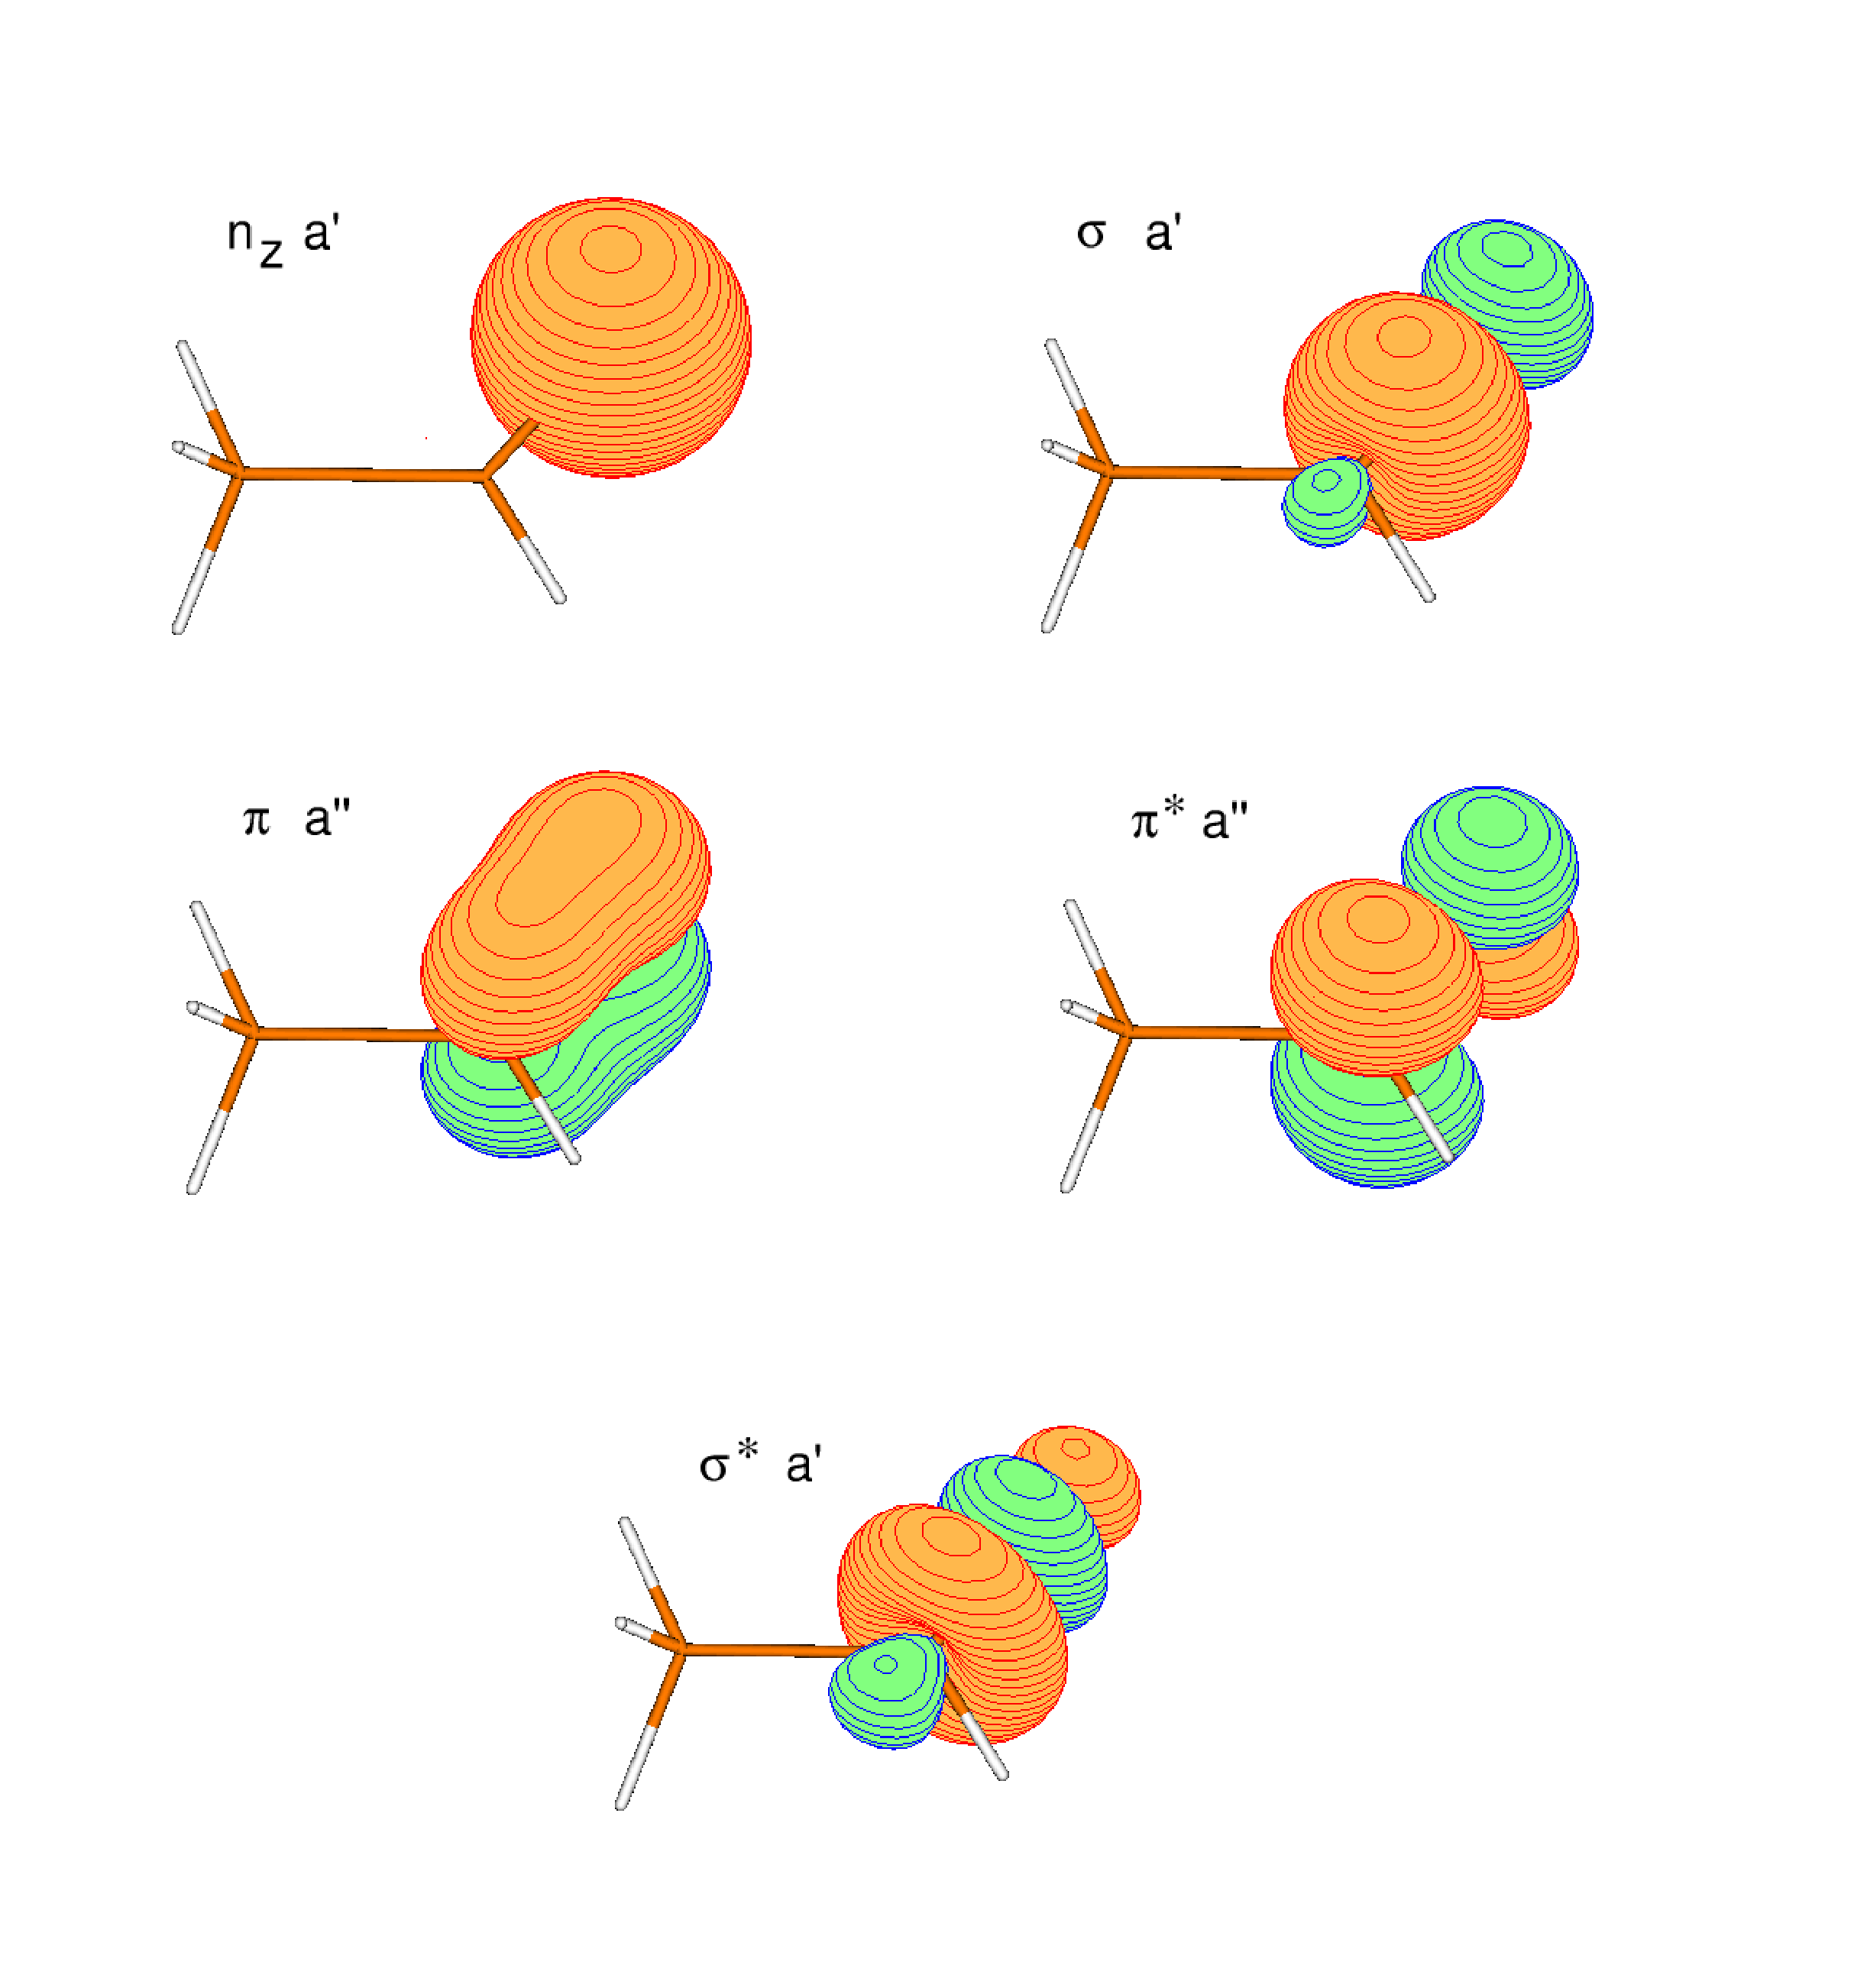
\includegraphics[width=9cm,keepaspectratio]{immagini/acetaldeide/orbitali_5.eps}
\end{center}
\end{figure}

\clearpage
Come \`e possibile notare, lo spazio attivo per lo stato fondamentale
\`e diverso da quello atteso: l'orbitale $n_y$ \`e stato
sostituito dall'orbitale $n_z$.

La ragione di tale variazione \`e imputabile al metodo di convergenza
dell'algoritmo CASSCF, che trova una migliore via di ottimizzazione (con
conseguente maggiore ottimizzazione variazionale dell'energia) attraverso
l'inclusione, nello spazio attivo, dell'orbitale $n_z$ anzich\'e dell'orbitale
$n_y$. Nei casi precedentemente trattati formaldeide e acetone, la simmetria
permetteva un controllo maggiore, in quanto gli orbitali $n_y$ ed $n_z$
appartenevano a rappresentazioni differenti.

Al contrario, lo stato eccitato di simmetria A$^{\prime\prime}$ ha il
corretto spazio attivo, in quanto il maggior contributo correlativo viene
ottenuto includendo gli orbitali interessati al fenomeno, e l'algoritmo
di ricerca del minimo energetico sceglie uno spazio fisicamente corretto.

Come conseguenza di tale errore, l'energia dello stato fondamentale \`e
troppo ottimizzata, perch\'e pi\`u bassa rispetto allo stato contenente
l'orbitale $n_y$ nello spazio attivo. Ne risulta perci\`o un'energia di
eccitazione sia verticale che adiabatica troppo alta.

Sebbene quindi uno spazio attivo cos\`i designato sia errato per questo tipo
di calcolo, la medesima strategia attuata su formaldeide e acetone \`e stata
attuata anche sull'acetaldeide, per meglio valutare come il metodo
perturbativo non sia in grado di porre rimedio ad una intrinseca incorretta
descrizione di uno degli stati di interesse. 
Seguir\`a uno studio ulteriore sulla molecola di
acetaldeide con uno spazio CAS allargato a 5 orbitali A$^{\prime}$ e 2
orbitali A$^{\prime\prime}$, che contenendo interamente la fisica di
interesse dovrebbe fornire, ed in effetti fornisce, risultati sensibilmente
pi\`u accurati.

L'ottimizzazione geometrica, riferita alla disposizione degli atomi mostrata
in figura, ha fornito i dati in tabella \ref{tab:acetaldeide_geom}

\begin{figure}[ht]
\begin{center}
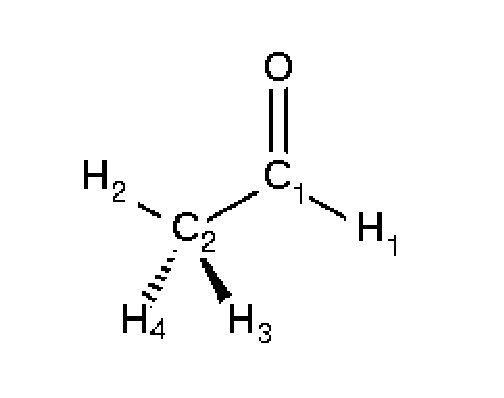
\includegraphics[angle=0,width=44mm,keepaspectratio]{immagini/acetaldeide/2d.eps}
\label{fig:acetaldeide_2d}
\end{center}
\end{figure}

\begin{center}
\begin{threeparttable}
\caption{\small Acetaldeide - geometria per lo stato fondamentale}
\label{tab:acetaldeide_geom}
\small
\begin{tabular}{|l|c|c|}
\hline
								& 6-311G*& Exp.\tnote{1} \\ %& 6-311G*/CAS $n_x \rightarrow \pistar$ \\
								& CAS(6,5)& 	 \\ %& 6-311G*/CAS $n_x \rightarrow \pistar$ \\
\hline
$r$(C$_1$-O)					& 1.21789		& 1.213 	\\%& 1.389869 \\
$r$(C$_1$-C$_2$)				& 1.50284		& 1.504		\\%& 1.497634 \\	
$r$(C$_1$-H$_1$)				& 1.09208		& 1.106		\\%& 1.078165 \\	
$r$(C$_2$-H$_2$)				& 1.08148		& 1.091		\\
$r$(C$_2$-H$_{3/4}$)			& 1.08588		& 1.085		\\
$\angle$(O-C$_1$-C$_2$)			& 124.007		& 124.0		\\%& 114.112 \\	
$\angle$(O-C$_1$-H$_1$)			& 119.395		& 121.1		\\%& 111.097 \\	
$\angle$(C$_2$-C$_1$-H$_1$)		& 116.598		& 114.9		\\%& 120.477 \\	
$\angle$(C$_1$-C$_2$-H$_{3/4}$)	& 110.148		& 110.6		\\%& 		 \\	
$\angle$(C$_1$-C$_2$-H$_2$)		& 110.347		& 110.6		\\%& 		 \\	
$\angle$(H$_3$-C$_2$-H$_4$)		& 107.232	 	&		\\%& 		 \\	
$\angle$(H$_2$-C$_2$-H$_{3/4}$)	& 109.454 		&		\\%& 		 \\	
$\tau$(O-C$_1$-C$_2$-H$_{3/4}$)	& $\pm120.959$	&		\\%& 		 \\	
\hline
\end{tabular}
\begin{tablenotes}
\small
 \item[1] Cfr. \cite{jpc-97-17-1993-4293}
 \item[] Distanze in Angstroms, angoli in gradi.
\end{tablenotes}
\end{threeparttable}
\end{center}

L'energia CASSCF a questa geometria \`e -153.024830 Hartree.
La transizione \mbox{$n_y \rightarrow \pistar$}, di simmetria $A^{\prime\prime}$,
ha energia CASSCF di -152.849283 Hartree. Conseguentemente, l'energia di transizione risulta essere 4.78 eV, contro
un valore sperimentale di 4.28 eV (Cfr. \cite{cpl-241-0-1995-26}).
Nel caso della transizione adiabatica, l'energia dello stato eccitato \`e -152.883379 Hartree, con una energia
di transizione pari a 3.85 eV, contro un valore sperimentale di 3.69 eV (Cfr. \cite{jpc-97-17-1993-4293})
La geometria di tale stato eccitato \`e mostrata in tabella \ref{tab:acetaldeide_geometrie_adiab}

\begin{center}
\begin{threeparttable}
\caption{\small Acetaldeide - geometria per lo stato eccitato adiabatico}
\label{tab:acetaldeide_geometrie_adiab}
\small
\begin{tabular}{|l|c|c|}
\hline
								& GS			&  $n_y \rightarrow \pistar$ \\ 
\hline
$r$($C_1$-O)					& 1.21789		& 1.38987 	\\
$r$($C_1$-$C_2$)				& 1.50284		& 1.49764	\\
$r$($C_1$-$H_1$)				& 1.09208		& 1.07816	\\
$r$($C_2$-$H_2$)				& 1.08148		& 1.08435	\\
$r$($C_2$-$H_3$)				& 1.08588		& 1.08290	\\
$r$($C_2$-$H_4$)				& 1.08588		& 1.08783	\\
$\angle$(O-$C_1$-$C_2$)			& 124.007		& 114.112	\\
$\angle$(O-$C_1$-$H_1$)			& 119.395		& 111.096	\\
$\angle$($C_1$-$C_2$-$H_1$)		& 116.598		& 120.478	\\
$\angle$($C_1$-$C_2$-$H_3$)		& 110.148		& 110.128	\\
$\angle$($C_1$-$C_2$-$H_4$)		& 110.148		& 111.455	\\
$\angle$($C_1$-$C_2$-$H_2$)		& 110.347		& 110.788   \\
$\angle$($H_3$-$C_2$-$H_4$)		& 107.232		& 108.365	\\
$\angle$($H_2$-$C_2$-$H_3$)		& 109.454		& 108.093	\\
$\angle$($H_2$-$C_2$-$H_4$)		& 109.454		& 107.902	\\
$\tau$(O-$C_1$-$C_2$-$H_4$)		& 120.959		&  65.135	\\
$\tau$(O-$C_1$-$C_2$-$H_3$)		& -120.959		& -174.562	\\
$\tau$(O-$C_1$-$C_2$-$H_2$)		& 0.0			& -55.029 	\\
$\tau$($H_2$-$C_2$-$C_1$-$H_1$)	& 180.0			& 168.836 	\\
\hline
\end{tabular}
\begin{tablenotes}
\small
 \item[] Distanze in Angstroms, angoli in gradi.
\end{tablenotes}
\end{threeparttable}
\end{center}
\subsubsection{Perturbazione su uno spazio CAS 6 elettroni/5 orbitali}

La tabella \ref{tab:acetaldeide_vertical_basis_5} presenta i risultati
ottenuti su un CAS con 6 elettroni in 5 orbitali, spazio CAS che, come gi\`a
enunciato, \`e errato in quanto descrive i due stati in modo sbilanciato.

\begin{center}
\begin{threeparttable}
\caption{\small Acetaldeide - Energia di transizione verticale {$n_y \rightarrow \pistar$} di singoletto, CAS 6 elettroni 5 orbitali}
\label{tab:acetaldeide_vertical_basis_5}
\small
\begin{tabular}{|c|ccc|ccc|}
\hline
Basis	& \multicolumn{3}{c|}{GS\tnote{1}}				& \multicolumn{3}{c|}{$n_y \rightarrow \pistar$ vert.\tnote{2}} \\
		& CASSCF		& NEV-PT	 	&	NEV-PT		& CASSCF		& NEV-PT	& NEV-PT  \\
		& 				& SC 			&	PC			& 				& SC		& PC 	 \\
\hline
6-31G	& 0.925561		& 1.143647		&	1.145329	& 4.19			& 4.07 		& 4.06	\\
cc-pVDZ	& 1.002377	 	& 1.380037		&	1.382306	& 4.74			& 4.49 		& 4.49	\\
ano-1	& 1.040915	 	& 1.415777		&	1.418769	& 4.74			& 4.51 		& 4.49	\\
6-311G*	& 1.024830	 	& 1.454798		&	1.457103	& 4.78			& 4.49 		& 4.50	\\
cc-pVTZ & 1.048304	 	& 1.568727		&	1.571395	& 4.78			& 4.48 		& 4.47	\\			
\hline
\hline
Exp.\tnote{3}&				& 				& 				& \multicolumn{3}{c|}{4.28} \\
\hline
\end{tabular}
\begin{tablenotes}
 \item[1] Energia come -(152 + valore) Hartree
 \item[2] Valori in eV
 \item[3] Cfr. \cite{jpc-97-17-1993-4293}
\end{tablenotes}
\end{threeparttable}
\end{center}

Come \`e possibile vedere, nonostante l'applicazione della trattazione
perturbativa, il risultato calcolato \`e ancora distante dal valore
sperimentale. Analogo risultato si ottiene dalla comparazione dei
valori per la transizione adiabatica

\begin{center}
\begin{threeparttable}
\caption{\small Acetaldeide - Energia di transizione adiabatica $n_y \rightarrow \pistar$ di singoletto, CAS 6 elettroni 5 orbitali}
\label{tab:acetaldeide_adiab_basis_5}
\small
\begin{tabular}{|c|ccc|ccc|}
\hline
Basis	& ZPE 			& ZPE 			& $\Delta$ZPE		& CASSCF	& NEV-PT			& NEV-PT  \\
		& 	(GS)		&  (Ecc.) 		& 					& ZPE		& SC/ZPE			& PC/ZPE  \\
\hline
6-31G	& 1.612			& 1.546			& -0.066			& 3.35			& 3.33			& 3.34 \\
cc-pVDZ & 1.593			& 1.534			& -0.059			& 3.78 			& 3.76			& 3.78 \\
ano-1	& 1.603			& 1.545			& -0.058			& 3.78			& 3.75 			& 3.77 \\
6-311G* & 1.600			& 1.545			& -0.055			& 3.79			& 3.78			& 3.80 \\
cc-pVTZ & 1.589			& 1.533			& -0.056			& 3.81			& 3.84			& 3.86 \\
\hline
\hline
Exp.\tnote{1}&				& 				& 					& \multicolumn{3}{c|}{3.69} \\
\hline
\end{tabular}
\begin{tablenotes}
 \item[1] Cfr. \cite{jpc-97-17-1993-4293}
 \item[ ] Valori in eV
\end{tablenotes}
\end{threeparttable}
\end{center}

Diagrammando le energie di transizione per questo caso, risulta ancora pi\`u
evidente come l'errore rispetto al dato sperimentale sia elevato, sia per la
transizione verticale che per quella adiabatica.

\begin{figure}[ht]
\begin{center}
\includegraphics[angle=270,width=10cm,keepaspectratio]{immagini/acetaldeide/energie_vert_5.eps} \\
\includegraphics[angle=270,width=10cm,keepaspectratio]{immagini/acetaldeide/energie_adiab_5.eps}
\parbox[h]{12cm}{
\caption{\small Acetaldeide - energia di transizione verticale (in alto) ed adiabatica (sopra) su basi differenti a livello CASSCF (linea rossa), NEV-PT/SC (linea verde) e NEV-PT/PC (linea blu) come funzione della base atomica.}
\label{fig:acetaldeide_energie_vert_5}
}
\end{center}
\end{figure}
\clearpage

\`E inoltre evidente come la trattazione perturbativa NEV-PT non riesca ad
effettuare una correzione significativa, in quanto lo scarto rispetto allo
sperimentale \`e causato da una differente natura fisica dello stato
fondamentale, sul quale la trattazione perturbativa non pu\`o recuperare.


\subsection{Acetaldeide - CAS 10 elettroni / 7 orbitali}

Al fine di migliorare la trattazione sull'acetaldeide, si \`e quindi scelto
uno spazio attivo compatibile con la necessit\`a di includere il doppietto $n_y$
sia nello stato fondamentale che nello stato eccitato.

La scelta ha portato ad ampliare lo spazio attivo, fino ad avere
5 orbitali A$^{\prime}$ e 2 orbitali A$^{\prime\prime}$,
e uno spazio di core costituito da 6 orbitali di simmetria A$^{\prime}$
e 1 orbitale di simmetria A$^{\prime\prime}$.
Con questa definizione, sono necessarie 106 configurazioni
nell'espansione CAS-CI, contro le 28 del precedente spazio attivo.

I risultati ottenuti sono rappresentati in tabella \ref{tab:acetaldeide_vertical_basis_7}
\begin{center}
\begin{threeparttable}
\caption{\small Acetaldeide - Energia di transizione verticale $n_y \rightarrow \pistar$ di singoletto, CAS 10 elettroni 7 orbitali}
\label{tab:acetaldeide_vertical_basis_7}
\small
\begin{tabular}{|c|ccc|ccc|}
\hline
Basis	& \multicolumn{3}{c|}{GS\tnote{1}}				& \multicolumn{3}{c|}{$n_y \rightarrow \pistar$ vert.\tnote{2}} \\
		& CASSCF		& NEV-PT	 	&	NEV-PT		& CASSCF		& NEV-PT	& NEV-PT	  \\
		& 				& SC 			&	PC			& 				& SC		& PC	 	 \\
\hline
6-31G	& 0.927916		& 1.138181		&	1.140489	& 4.06			& 4.01		& 4.03		\\
cc-pVDZ	& 1.004396		& 1.370583		&	1.373364	& 4.58			& 4.37		& 4.38		\\
ano-1	& 1.042885		& 1.405010		&	1.408962	& 4.59			& 4.35 		& 4.34		\\
6-311G*	& 1.026837		& 1.445053		&	1.447570	& 4.62			& 4.35		& 4.37		\\
cc-pVTZ & 1.050199		& 1.556482		&	1.559922	& 4.62			& 4.32		& 4.32		\\			
\hline
\hline
Exp.\tnote{3}&				& 				& 				& \multicolumn{3}{c|}{4.28} \\
\hline
\end{tabular}
\begin{tablenotes}
 \item[1] Energia come -(152 + valore) Hartree
 \item[2] Valori in eV
 \item[3] Cfr. \cite{jpc-97-17-1993-4293}
\end{tablenotes}
\end{threeparttable}
\end{center}

\`E evidente come, con uno spazio attivo allargato, si venga incontro alla
necessit\`a fisica di descrivere lo stato fondamentale e quello eccitato
nello stesso modo. I valori per la transizione a livello CAS restano
tuttavia relativamente distanti dal valore vero di 4.28 eV, nonostante il
numero di configurazioni sia considerevolmente aumentato. La perturbazione
consente di recuperare parte dell'energia di correlazione ed avvicinarsi
cos\`i in modo pi\`u deciso all'energia di transizione sperimentale.

Analoghe considerazioni per quanto riguarda la transizione adiabatica,
i cui risultati sono riportati in tabella \ref{tab:acetaldeide_adiab_basis_7}

\begin{center}
\begin{threeparttable}
\caption{\small Acetaldeide - Energia di transizione adiabatica $n_y \rightarrow \pistar$ di singoletto, CAS 10 elettroni 7 orbitali}
\label{tab:acetaldeide_adiab_basis_7}
\small
\begin{tabular}{|c|ccc|ccc|}
\hline
Basis	& ZPE 			& ZPE 			& $\Delta$ZPE		& CASSCF		& NEV-PT		& NEV-PT	 \\
		& (GS)			& (Ecc.) 		& 					& ZPE			& SC/ZPE		& PC/ZPE 	 \\
\hline
6-31G	& 1.612			& 1.544			& -0.068			& 3.32			& 3.30			& 3.33			 \\
cc-pVDZ & 1.592			& 1.531			& -0.062			& 3.73 			& 3.64			& 3.66			 \\
ano-1	& 1.603			& 1.542			& -0.060			& 3.73			& 3.60 			& 3.61			 \\
6-311G* & 1.600 		& 1.543			& -0.057			& 3.74			& 3.65			& 3.66			 \\
cc-pVTZ & 1.590			& 1.531			& -0.059			& 3.76			& 3.68			& 3.69			 \\
\hline
\hline
Exp.\tnote{1}&				& 				& 					& \multicolumn{3}{c|}{3.69} \\
\hline
\end{tabular}
\begin{tablenotes}
 \item[1] Cfr. \cite{jpc-97-17-1993-4293}
 \item[] Valori in eV
\end{tablenotes}
\end{threeparttable}
\end{center}

Come si pu\`o vedere, c'\`e un ottimo accordo tra il dato sperimentale e il
valore calcolato, gi\`a buono a livello CAS, che viene migliorato ulteriormente
dall'applicazione della perturbazione.

Al solito, i grafici \ref{fig:acetaldeide_energie_vert_7} e \ref{fig:acetaldeide_energie_adiab_7}
mostrano l'andamento dei dati sopra rappresentati, permettendo di
evidenziare in modo pi\`u netto l'andamento delle energie di transizione
verticale e adiabatica
\begin{figure}[ht]
\begin{center}
\includegraphics[angle=270,width=11cm,keepaspectratio]{immagini/acetaldeide/energie_vert_7.eps}
\parbox[h]{12cm}{
\caption{\small Acetaldeide - energia di transizione verticale su basi differenti a livello CASSCF (linea rossa), NEV-PT/SC (linea verde) e NEV-PT/PC (linea blu) come funzione della base atomica.}
\label{fig:acetaldeide_energie_vert_7}
}
\end{center}
\end{figure}
\pagebreak
\begin{figure}[ht]
\begin{center}
\includegraphics[angle=270,width=12cm,keepaspectratio]{immagini/acetaldeide/energie_adiab_7.eps}
\parbox[h]{12cm}{
\caption{\small Acetaldeide - energia di transizione adiabatica su basi differenti a livello CASSCF (linea rossa), NEV-PT/SC (linea verde) e NEV-PT/PC (linea blu) come funzione della base atomica.}
\label{fig:acetaldeide_energie_adiab_7}
}
\end{center}
\end{figure}

\clearpage


\section{Sistemi coniugati ciclici}

Lo studio degli stati eccitati \`e proseguito con un'analisi 
delle molecole coniugate cicliche di benzene e naftalene, con
diverse basi orbitaliche.

\subsection{Benzene}

La molecola di benzene, di simmetria D$_{6h}$ \`e stata caratterizzata nello
stato fondamentale e negli stati eccitati di singoletto appartenenti alle rappresentazioni
B$_{2u}$ e B$_{1u}$. A causa di imposizioni del programma \texttt{dalton},
si \`e lavorato con il sottogruppo D$_{2h}$.

Inizialmente si \`e condotto un calcolo esplorativo, su base 6-31G* con spazio
CAS 6/6 definito dagli orbitali $\pi$ e dai corrispondenti $\pistar$. Tale
calcolo ha fornito geometrie e valutazioni degli orbitali e delle loro
simmetrie.

In seguito, per affinare i risultati, si \`e provveduto ad effettuare altre
valutazioni, passando quindi alla base ano-1 definita 3s2p1d per il carbonio
e 2s1p per l'idrogeno, sia con il medesimo spazio CAS sopra descritto, sia
con uno spazio CAS ampliato, ottenuto raddoppiando gli orbitali per ogni
simmetria, e passando di conseguenza ad un CAS 6/12.

La molecola \`e stata posta sul piano $xy$, con l'asse principale orientato
lungo l'asse $z$.

I ben noti orbitali $\pi$ del benzene, orbitali che faranno parte dello
spazio attivo non espanso, in simmetria D$_{6h}$ sono assegnabili alle
rappresentazioni A$_{2u}$, E$_{1g}$, E$_{2u}$ e B$_{2g}$. In simmetria
D$_{2h}$ tali rappresentazioni si trasformano, rispettivamente e ricordando
che le rappresentazioni E sono bidimensionali, in B$_{1u}$, B$_{2g}$,
B$_{3g}$, B$_{1u}$, A$_{u}$ e B$_{2g}$. Gli orbitali appartenenti alle prime
tre rappresentazioni sono occupati.
Sempre in seguito alla diminuzione di simmetria, gli stati eccitati su cui
verranno effettuate valutazioni apparterranno, in simmetria D$_{2h}$,
alle rappresentazioni B$_{2u}$ e B$_{3u}$, anzich\'e B$_{2u}$ e B$_{1u}$,
rispettivamente, per la simmetria D$_{6h}$.

Le geometrie molecolari sono state ottimizzate nelle varie condizioni
operative. Nella tabella \ref{tab:benzene_geom} sono messe a confronto le
geometrie ottenute per via teorica con il dato sperimentale
\begin{center}
\begin{threeparttable}
\caption{\small Benzene - geometrie su diversi metodi/basi}
\label{tab:benzene_geom}
\small
\begin{tabular}{|l|c|c|}
\hline
							& R$_{CC}$		& R$_{CH}$ \\ 
\hline
CASSCF 6/6 / 6-31G*			& 1.396			&	1.075	 \\
CASSCF 6/6 / ano-1			& 1.398			&	1.080	 \\
CASSCF 6/12 / ano-1			& 1.398			&	1.081    \\
Exp.\tnote{1}				& 1.390			&	1.086    \\
\hline
\end{tabular}
\begin{tablenotes}
\small
 \item[1] Cfr. \cite{jms-148-1991-427}
 \item[] Valori in Angstroms
\end{tablenotes}
\end{threeparttable}
\end{center}

\subsubsection{Eccitazione B$_{2u}$ (B$_{2u}$ in D$_{2h}$)}

La transizione elettronica B$_{2u}$ \`e quella a minore energia. Analisi
sperimentali (Cfr. \cite{jcp-94-12-1991-7700}) forniscono per questa
transizione un valore di 4.90 eV, anche se in realt\`a lo spettro in fase gas
e jet-cooled forniscono un inviluppo vibrazionale che va da 4.79 eV
(transizione 0-0) fino a 5.35 eV, con un picco di massimo assorbimento
proprio a 4.90 eV, scelto come riferimento per la transizione Franck-Condon.

La tabella \ref{tab:benzene_b2u} mostra i risultati ottenuti con la
trattazione effettuata.
\begin{center}
\begin{threeparttable}
\caption{\small Benzene - Energia della transizione di singoletto B$_{2u}$
(B$_{2u}$ in D$_{2h}$)}
\label{tab:benzene_b2u}
{
\small
\begin{tabular}{|c|ccc|ccc|}
\hline
 				& \multicolumn{3}{c|}{GS\tnote{1}}				& \multicolumn{3}{c|}{Ecc. B$_{2u}$\tnote{2}} \\
				& CASSCF	& NEV-PT	& NEV-PT	& CASSCF		& NEV-PT	& NEV-PT \\
				&			& SC		& PC		& 				& SC		& PC \\
\hline
CAS(6,6)/6-31G*	& 0.775778	& 1.468765	& 1.469361	& 4.99			& 5.33		& 5.31		\\
CAS(6,6)/ano-1	& 0.830416	& 1.558968	& 1.559728	& 4.92			& 5.22		& 5.20		\\
CAS(6,12)/ano-1	& 0.844274	& 1.558662	& 1.564030	& 4.92			& 5.17		& 5.19		\\
\hline
\hline
Exp.\tnote{3}	&				& 				&				& \multicolumn{3}{c|}{4.90} \\
\hline
\end{tabular}
}
\begin{tablenotes}
\small
 \item[1] Energia come \mbox{-(230 + valore)} Hartree
 \item[2] Valori in eV
 \item[3] Cfr. \cite{jcp-94-12-1991-7700}
\end{tablenotes}
\end{threeparttable}
\end{center}

Apparentemente quindi, il risultato CASSCF \`e in buon accordo con il dato
sperimentale, e la trattazione perturbativa attua un allontanamento dal
valore esatto. Tuttavia, la Ref. \cite{jcp-112-6-2000-2798} sottolinea come
la differenza tra la transizione 0-0 ed il massimo della banda sia 0.19 eV,
mentre sui valori calcolati la differenza tra la transizione 0-0 e la
verticale \`e di 0.31 eV. Di conseguenza, il massimo della banda \`e spostato
di 0.12 eV pi\`u in basso rispetto all'energia verticale Franck-Condon.
Questo implica che il valore sperimentale di 4.90 eV comporta, per la
transizione verticale, un posizionamento a 5.02 eV, in migliore accordo
con i dati ottenuti a livello perturbativo.

\subsubsection{Eccitazione B$_{1u}$ (B$_{3u}$ in D$_{2h}$)}

La transizione B$_{1u}$ viene stimata attorno ai 6.20 eV (Cfr.
\cite{jcp-112-6-2000-2798} e \cite{tca-91-1995-91}). La tabella
\ref{tab:benzene_b1u} mostra i dati ottenuti
\begin{center}
\begin{threeparttable}
\caption{\small Benzene - Energia della transizione di simmetria B$_{1u}$
(B$_{3u}$ in D$_{2h}$)}
\label{tab:benzene_b1u}
{
\small
\begin{tabular}{|c|ccc|}
\hline
 				& \multicolumn{3}{c|}{ Ecc. B$_{1u}$\tnote{2}} \\
				& CASSCF		& NEV-PT/SC & NEV-PT/PC \\
\hline
CAS(6,6)/6-31G*	&  8.18			& 6.75		& 6.71		\\
CAS(6,6)/ano-1	&  7.87			& 6.33 		& 6.26		\\
CAS(6,12)/ano-1	&  7.46			& 6.54		& 6.50		\\
\hline
\hline
Exp.\tnote{3}	&	 \multicolumn{3}{c|}{6.20} \\
\hline
\end{tabular}
}
\begin{tablenotes}
\small
 \item[1] Valori in Hartree
 \item[2] Valori in eV
 \item[3] Cfr. \cite{jcp-112-6-2000-2798} e \cite{tca-91-1995-91}
\end{tablenotes}
\end{threeparttable}
\end{center}

\subsection{Naftalene}

Analoga trattazione \`e stata eseguita sul naftalene, molecola di simmetria
D$_{2h}$.
La molecola \`e stata orientata sul piano $xy$, con l'asse C$_2$ ortogonale al
piano molecolare lungo l'asse $z$.
Il calcolo \`e stato eseguito con base 6-31G* con spazio CAS 10 elettroni in
10 orbitali $\pi$ (per un totale di 4936 configurazioni) e successivamente
con base ano-1 definita 3s2p1d per il carbonio e 2s1p per l'idrogeno. Gli
orbitali facenti parte dello spazio attivo sono caratterizzati dalle
simmetrie B$_{1u}$, B$_{2g}$, B$_{3g}$, B$_{1u}$, A$_u$, B$_{2g}$, B$_{3g}$,
B$_{1u}$, A$_u$ e B$_{3g}$.  A livello HF, solo i primi 5 orbitali
(b$_{1u}$, b$_{2g}$, b$_{3g}$, b$_{1u}$, a$_u$) sono occupati.

La geometria \`e stata ottimizzata su entrambe le basi. Data l'assegnazione
per i legami data in figura

\begin{figure}[ht]
\begin{center}
\includegraphics[angle=0,width=4cm,keepaspectratio]{immagini/naftalene/geom.eps}
\end{center}
\end{figure}

i risultati, confrontati con il valore sperimentale (Cfr. \cite{prsls-258-1960-270})
sono visibili in tabella \ref{tab:naftalene_geom}
\begin{center}
\begin{threeparttable}
\caption{\small Naftalene - geometrie su diverse basi}
\label{tab:naftalene_geom}
\small
\begin{tabular}{|l|c|c|c|}
\hline
					& 6-31G*	& ano-1		&	Exp.\tnote{1}	\\ 
\hline
$r_1$				& 1.427		& 1.427		&	1.421	\\
$r_2$				& 1.373		& 1.375		&	1.364	\\
$r_3$				& 1.421		& 1.424		&	1.415	\\
$r_4$				& 1.416		& 1.415		&	1.418	\\
\hline
\end{tabular}
\begin{tablenotes}
\small
 \item[1] Cfr. \cite{prsls-258-1960-270}
 \item[] Valori in Angstroms
\end{tablenotes}
\end{threeparttable}
\end{center}

\subsubsection{Eccitazione B$_{3u}$}

La transizione elettronica che origina lo stato eccitato di simmetria
B$_{3u}$ risulta essere quella con minima energia. Il valore sperimentale
(Cfr. \cite{cpl-16-1972-464} e \cite{jms-26-1968-67}) \`e assegnato a 4.0 eV.

La tabella \ref{tab:naftalene_b3u} mostra i risultati ottenuti con la
trattazione effettuata. Come si vede, I risultati risentono di un certo
errore rispetto al valore sperimentale.
\begin{center}
\begin{threeparttable}
\caption{\small Naftalene - Energia della transizione di simmetria B$_{3u}$. CAS
10/10 su basi differenti}
\label{tab:naftalene_b3u}
{
\begin{tabular}{|c|ccc|ccc|}
\hline
\small
 				& \multicolumn{3}{c|}{GS\tnote{1}}				& \multicolumn{3}{c|}{Ecc. B$_{3u}$\tnote{2}} \\
				& CASSCF		& NEV-PT		& NEV-PT		& CASSCF		& NEV-PT	& NEV-PT \\
				&				& SC			& PC			& 				& SC		& PC	 \\
\hline
6-31G*			& 0.477577		& 1.629822		& 1.631355		& 4.32			& 4.54		& 4.52	\\
ano-1			& 0.565924		& 1.776676		& 1.778645		& 4.29			& 4.46		& 4.43	\\
\hline
\hline
Exp.\tnote{3}	&				& 				&				& \multicolumn{3}{c|}{4.0} \\
\hline
\end{tabular}
}
\begin{tablenotes}
\small
 \item[1] Energia come \mbox{-(383 + valore)} Hartree
 \item[2] Valori in eV
 \item[3] Cfr. \cite{cpl-16-1972-464} e \cite{jms-26-1968-67}
\end{tablenotes}
\end{threeparttable}
\end{center}


\subsubsection{Eccitazione B$_{2u}$}

Per quanto riguarda l'eccitazione B$_{2u}$, i risultati sono decisamente
migliori. A livello CASSCF l'errore \`e elevato, pi\`u di 2 eV. L'applicazione
della perturbazione porta a risultati praticamente coincidenti con il range
accertato per lo sperimentale.

\begin{center}
\begin{threeparttable}
\caption{\small Naftalene - Energia della transizione di simmetria B$_{2u}$}
\label{tab:naftalene_b2u}
{
\small
\begin{tabular}{|c|ccc|}
\hline
 				& \multicolumn{3}{c|}{ Ecc. B$_{2u}$ \tnote{2}} \\
				& CASSCF		& NEV-PT & NEV-PT \\
				& 				& SC	 & PC \\
\hline
6-31G*	&  6.62			& 4.88	 &  4.82 \\
ano-1	&  6.42			& 4.51	 & 4.42	\\
\hline
\hline
Exp.\tnote{3} &	 \multicolumn{3}{c|}{4.45-4.7} \\
\hline
\end{tabular}
}
\begin{tablenotes}
\small
 \item[1] Valori in Hartree
 \item[2] Valori in eV
 \item[3] Cfr. \cite{cpl-16-1972-464}, \cite{jms-26-1968-67} e \cite{jpb-25-1992-2197}
\end{tablenotes}
\end{threeparttable}
\end{center}


\section{Sistemi coniugati lineari}

Per ultimo, lo studio di sistemi coniugati lineari si \`e invece concentrato
sull'esatriene, previa caratterizzazione analoga sull'omologo inferiore
minimale etilene che, pur non essendo a rigore un sistema coniugato, ha
consentito la valutazione essenziale dei parametri e dei risultati in
studio: si \`e valutata la superficie di potenziale per lo stato
fondamentale, definita sui due gradi di libert\`a della rotazione del doppio
legame centrale e della posizione degli idrogeni interessati a tale
rotazione. 

Successivamente, sul sistema esatriene si \`e studiato il percorso di minima
energia (Minimum Energy Path, MEP) e le energie di eccitazione verticale ed
adiabatica, e la conseguente trattazione perturbativa.

\subsection{Etilene}

L'etilene \`e stato scelto quale composto di riferimento per la descrizione
della superficie di potenziale descritta dai gradi di libert\`a di interesse.
Per descrivere la molecola si \`e fatto uso della base 6-31G*, con un CAS 2/2
comprendente gli orbitali $\pi$ e $\pistar$

\begin{figure}[ht]
\begin{center}
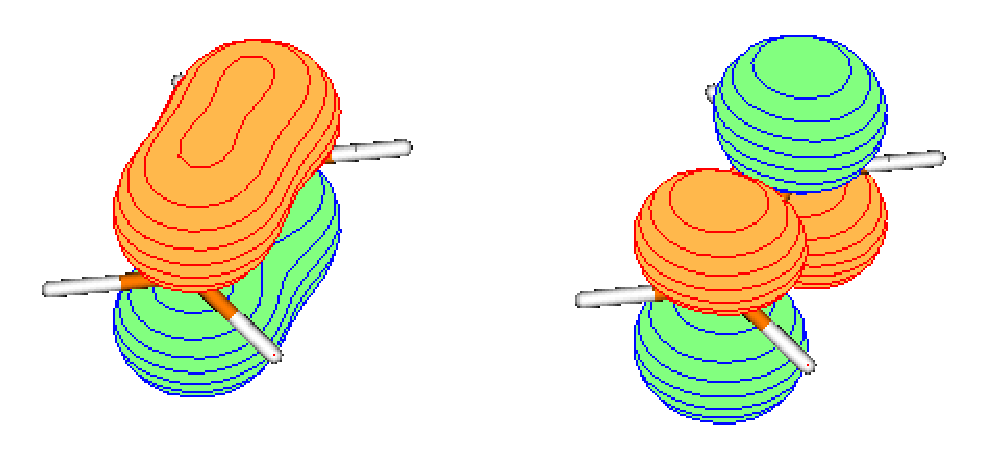
\includegraphics[angle=0,width=7cm,keepaspectratio]{immagini/etene/orbitali.eps}
\parbox[h]{10cm}{
\caption{\small Etilene - orbitali $\pi$ e $\pistar$}
\label{fig:etene_orbitali}
}
\end{center}
\end{figure}

I parametri geometrici in condizioni di equilibrio sono rappresentati in
tabella \ref{tab:etene_geom}, confrontati con un calcolo CASSCF
2/11 con base 6-311(2+)G* (Cfr . \cite{jcp-105-20-1996-9007})
\begin{center}
\begin{threeparttable}
\caption{\small Etilene - geometria per lo stato fondamentale}
\label{tab:etene_geom}
\small
\begin{tabular}{|ccc|c|}
\hline
							& GS		& GS CAS 2/11\tnote{1} \\ 
\hline
$r$(C-C)					& 1.338		& 1.338	\\
$r$(C-H)					& 1.076		& 1.076	 \\
$\angle$(H-C-C)				& 121.7		& 121.7	 \\
\hline
\end{tabular}
\begin{tablenotes}
\small
 \item[1] Cfr. \cite{jcp-105-20-1996-9007}
\end{tablenotes}
\end{threeparttable}
\end{center}

Facendo riferimento alla disposizione degli atomi data in figura
\begin{figure}[ht]
\begin{center}
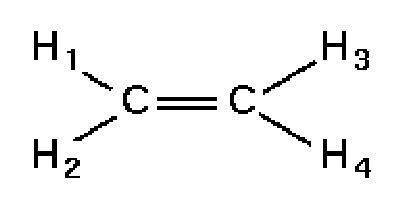
\includegraphics[angle=0,width=3cm,keepaspectratio]{immagini/etene/etene.eps}
\end{center}
\end{figure}
e assumendo che con angolo diedro A-B-C-D si intende l'angolo formato dai
piani definiti da A,B,C e B,C,D, la rotazione attorno al doppio legame 
viene studiata vincolando le torsioni H$_1$-C-C-H$_3$ e H$_2$-C-C-H$_4$, 
modificandone il valore da $0^{\circ}$ a $180^{\circ}$, ed eseguendo
l'ottimizzazione geometrica sui restanti gradi di libert\`a. Ne risulta
la superficie di potenziale, mostrata in figura \ref{fig:etene_3d}.

\begin{figure}[ht]
\begin{center}
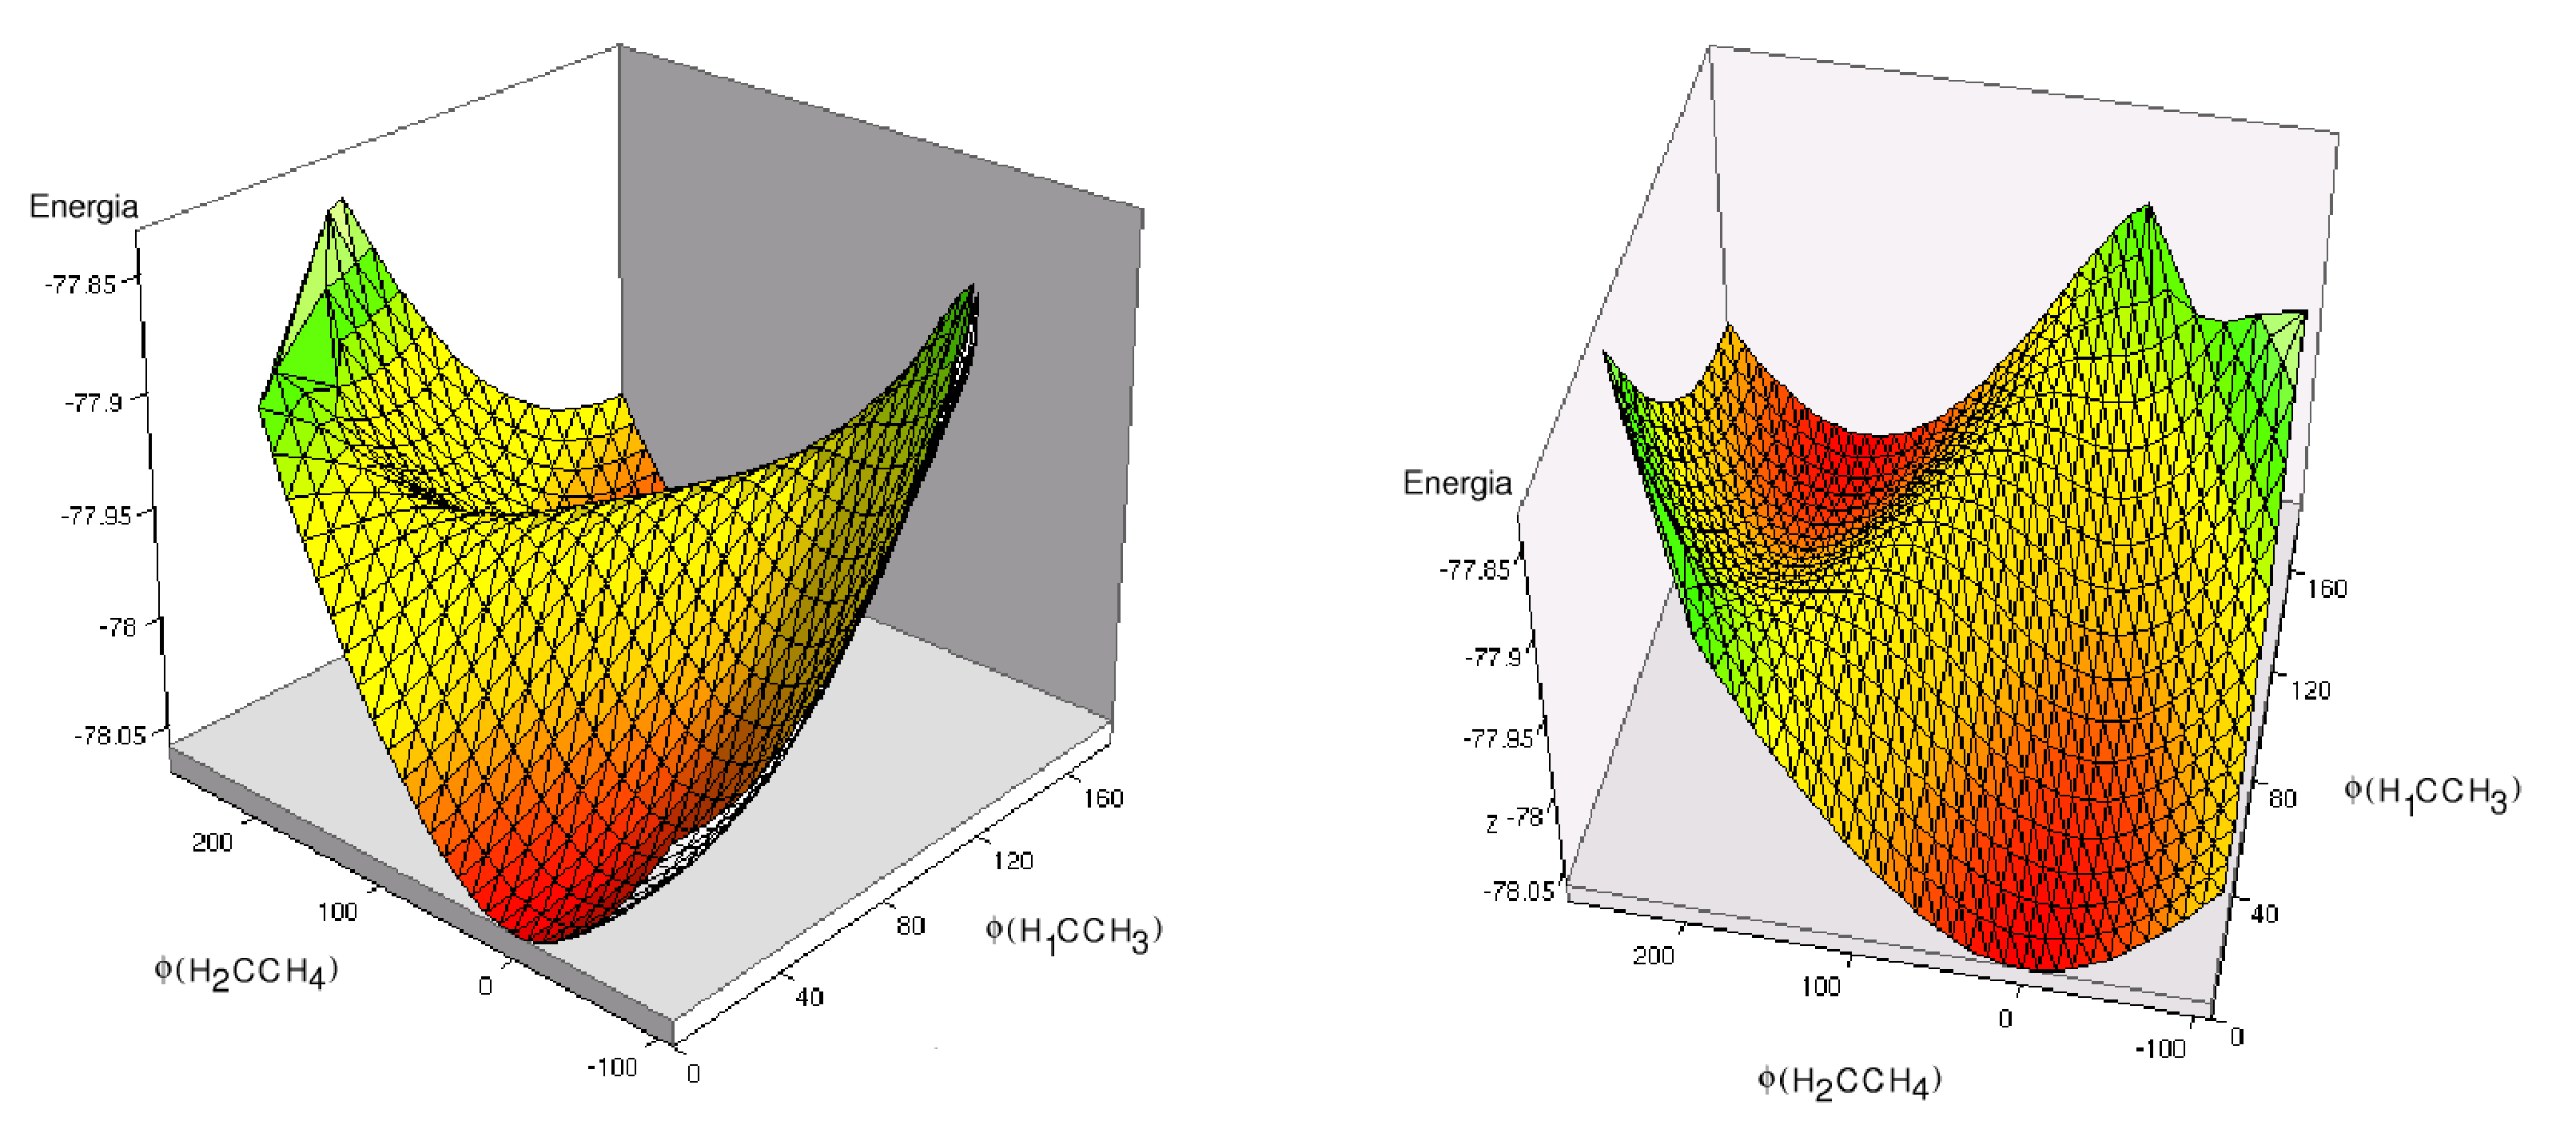
\includegraphics[angle=0,width=12cm,keepaspectratio]{immagini/etene/3d.eps}
\caption{\small Etilene - superfici di potenziale}
\label{fig:etene_3d}
\end{center}
\end{figure}

\`E possibile notare come tale superficie presenti due valli parallele,
ciascuna delle quali degenera in una spalla quando l'energia del minimo
diviene eccessivamente elevata. Una sezione della superficie a 
H$_1$-C-C-H$_3$ pari a 90$^{\circ}$ mostra un doppio minimo, con energie comparabili. 
\begin{figure}[ht]
\begin{center}
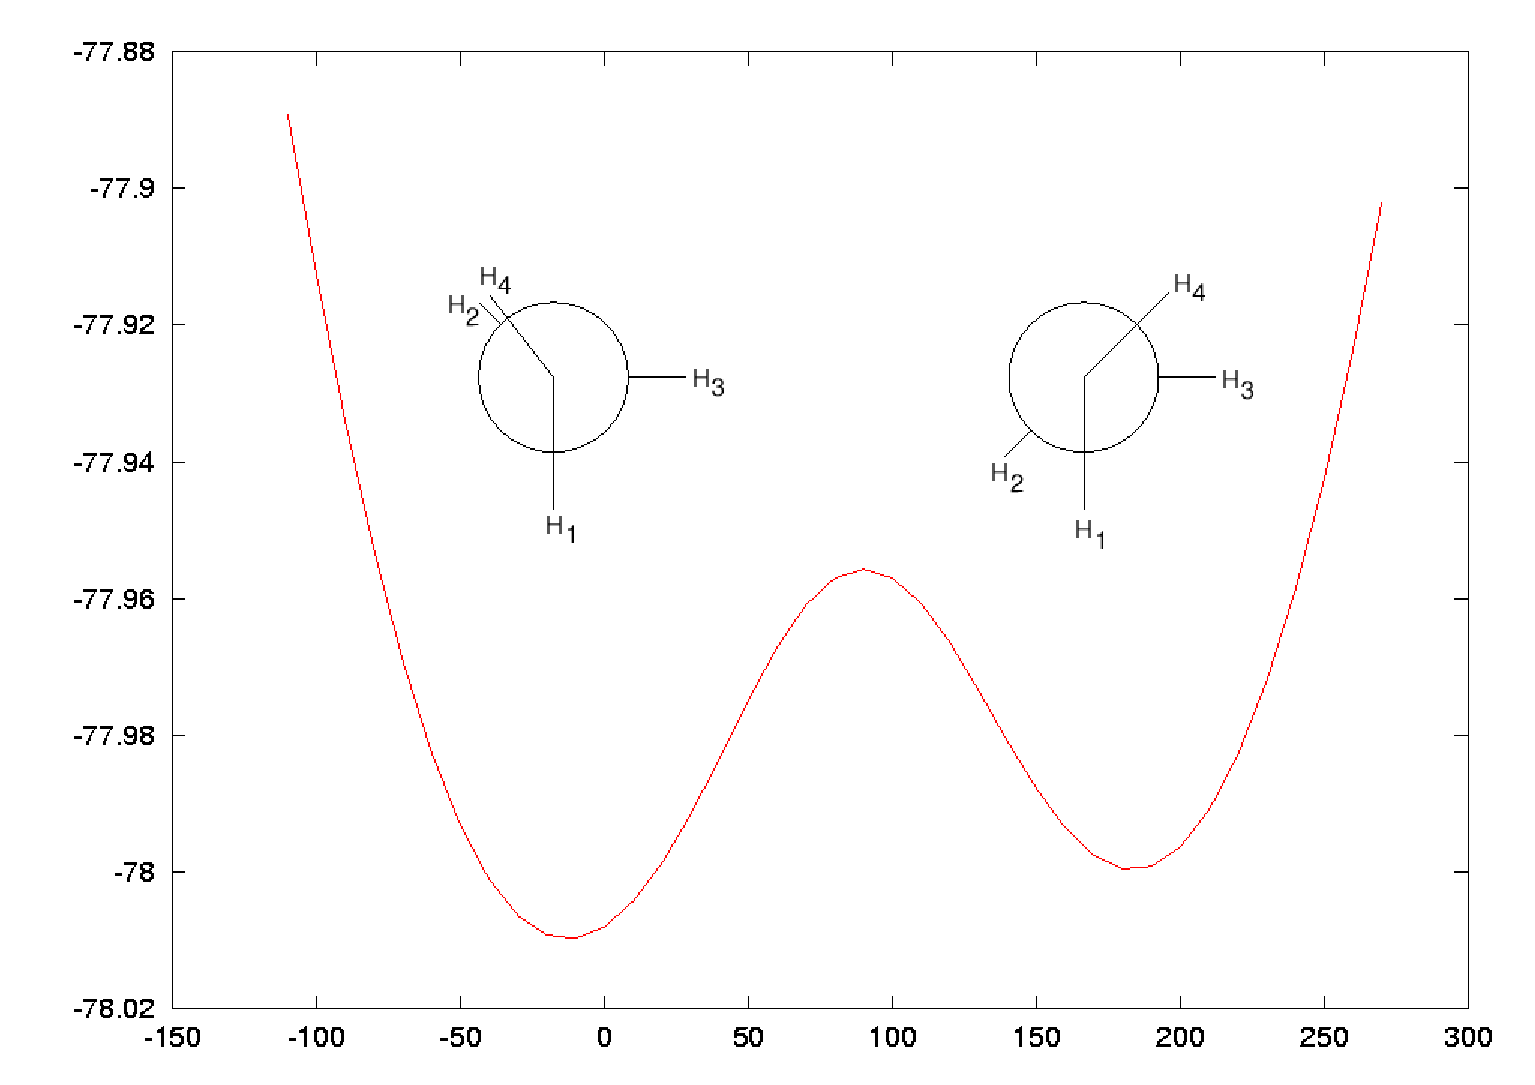
\includegraphics[angle=0,width=10cm,keepaspectratio]{immagini/etene/c090.eps}
\caption{\small Etilene - curva di potenziale rispetto all'angolo diedro
H$_2$-C-C-H$_4$. L'angolo diedro H$_1$-C-C-H$_3$ \`e fissato a 90$^{\circ}$}
\label{fig:etene_c090}
\end{center}
\end{figure}

Entrambi i minimi descrivono una possibile organizzazione spaziale a minima
energia della molecola in queste condizioni: la differenza, come \`e 
\begin{wrapfigure}{l}{6cm}
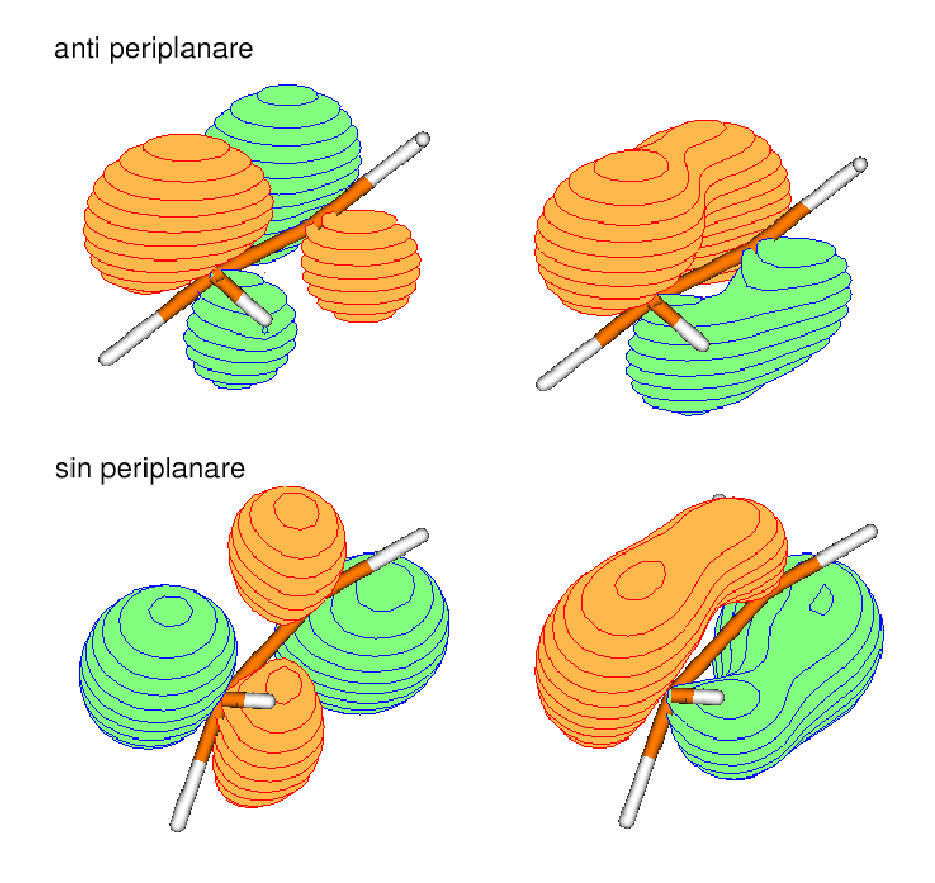
\includegraphics[angle=0,width=55mm,keepaspectratio]{immagini/etene/orbitali_c090.eps}
\caption{\small Etilene - orbitali dello spazio attivo (diedro H$_1$-C-C-H$_3$ a 90$^{\circ}$)}
\label{fig:etene_orbitali_c090}
\end{wrapfigure}
possibile notare dalla figura \ref{fig:etene_c090}, deriva dal diverso
posizionamento degli idrogeni H$_2$ e H$_4$, che assecondano i vincoli e la
necessit\`a di piramidalizzazione disponendosi in due diverse configurazioni
coplanari, una sin-periplanare, l'altra anti-periplanare. Il minimo
sin-periplanare possiede energia minore, anche a livello puramente nucleare,
sebbene presenti due atomi di idrogeno in posizione eclissata.
Gli orbitali attivi in queste due condizioni sono rappresentati in
figura \ref{fig:etene_orbitali_c090}.
La barriera di potenziale necessaria ad interconvertire, lungo questo grado
di libert\`a, la forma sin in forma anti \`e approssimativamente 1.45 eV, e passa per un
intermedio planare in cui gli orbitali $p$ degli atomi di carbonio sono
ortogonali.
L'utilizzo dell'etilene come esempio dimostrativo della superficie non
consente la distinzione tra isomero cis ed isomero trans, distinzione
che sar\`a apprezzabile nell'esatriene.


\subsection{Esatriene}

La molecola di esatriene \`e stata presa in esame sugli stessi parametri
dell'etilene, considerando la rotazione attorno al doppio legame centrale.

\begin{figure}[ht]
\begin{center}
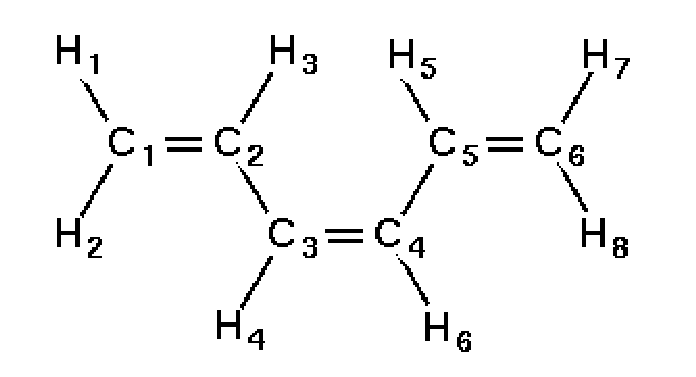
\includegraphics[angle=0,width=6cm,keepaspectratio]{immagini/esatriene/esatriene_cis.eps}
\end{center}
\end{figure}

Si \`e infatti valutata la superficie di potenziale associata ai due gradi di libert\`a
definiti dagli angoli diedri \mbox{C$_2$-C$_3$-C$_4$-C$_5$} e \mbox{H$_4$-C$_3$-C$_4$-H$_6$}.
La base usata per questa trattazione \`e la {6-31G*}. Lo spazio CAS \`e stato
definito in modo tale da includere 6 orbitali $\pi$ ed i corrispondenti
6 elettroni.
\begin{figure}[ht]
\begin{center}
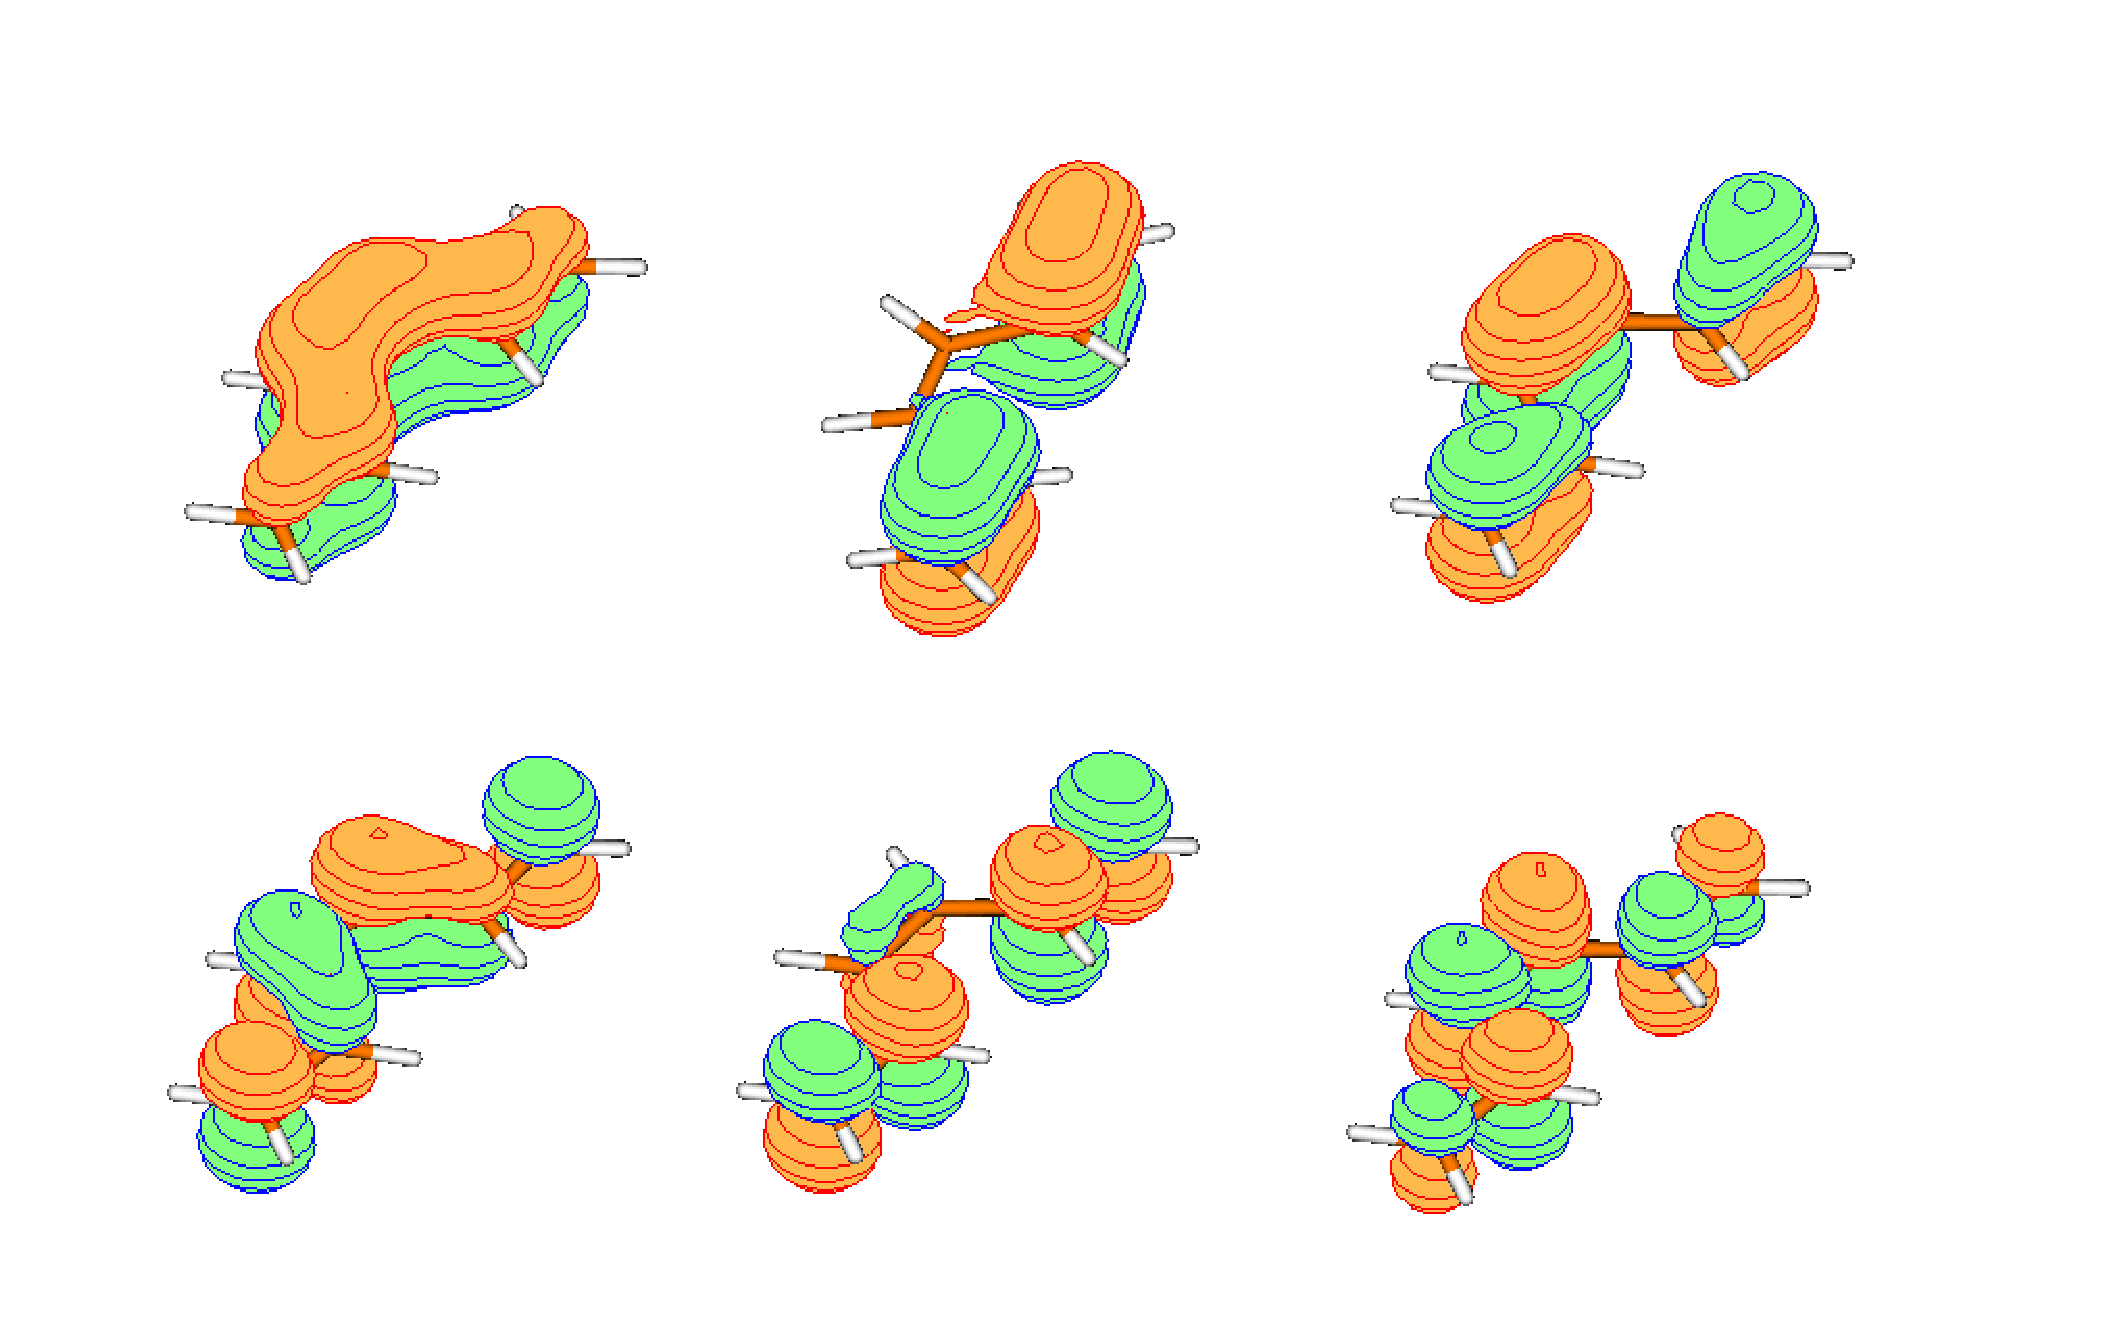
\includegraphics[angle=0,width=10cm,keepaspectratio]{immagini/esatriene/orbitali.eps}
\caption{\small Esatriene cis - orbitali nello spazio CAS 6/6}
\label{fig:esatriene_orbitali}
\end{center}
\end{figure}

\clearpage

La geometria dell'esatriene cis all'equilibrio \`e definita in tabella
\ref{tab:esatriene_geometrie}.
\begin{center}
\begin{threeparttable}
\caption{\small Esatriene cis - geometria stato fondamentale}
\label{tab:esatriene_geometrie}
\small
\begin{tabular}{|ccc|c|}
\hline
							& CASSCF	& Exp.\tnote{1} \\ 
\hline
$r$(C$_1$=C$_2$)			& 1.3456	& 1.336				\\
$r$(C$_2$-C$_3$)			& 1.4634	& 1.462				\\
$r$(C$_3$=C$_4$)			& 1.3537	& 1.362				\\
$r$(C$_1$-H$_1$)			& 1.0745	& 1.090				\\
$r$(C$_1$-H$_2$)			& 1.0763	& 1.090				\\
$r$(C$_2$-H$_3$)			& 1.0757	& 1.090				\\
$r$(C$_3$-H$_4$)			& 1.0775	& 1.090				\\
$\angle$(C$_1$C$_2$C$_3$)	& 123.293	& 122.1			 \\
$\angle$(C$_2$C$_3$C$_4$)	& 127.097	& 125.9		 \\
$\angle$(C$_2$C$_1$H$_1$)	& 121.546	& 124.0		 \\
$\angle$(C$_2$C$_1$H$_2$)	& 121.712	& 124.0		 \\
$\angle$(C$_4$C$_3$H$_4$)	& 117.476	& 118.0		 \\
$\angle$(C$_3$C$_2$H$_3$)	& 118.140	& 121.0		 \\
\hline
\end{tabular}
\begin{tablenotes}
\small
 \item[1] Cfr. \cite{jcp-114-4-2001-1631}
\end{tablenotes}
\end{threeparttable}
\end{center}

A tale geometria, ovviamente, gli angoli diedri \mbox{C$_2$-C$_3$-C$_4$-C$_5$} e
\mbox{H$_4$-C$_3$-C$_4$-H$_6$} sono entrambi pari a 0.

Successivamente si \`e proceduto ad effettuare la rotazione attorno al
doppio legame, facendo variare \mbox{C$_2$-C$_3$-C$_4$-C$_5$}. Per ragioni
strettamente numeriche la procedura seguita \`e stata differente da quella
ideale: dal punto di vista pratico si \`e partiti da una geometria gi\`a
ruotata, con diedro \mbox{C$_2$-C$_3$-C$_4$-C$_5$} pari a 90$^{\circ}$ e
diedro \mbox{H$_4$-C$_3$-C$_4$-H$_6$} pari a 0$^{\circ}$, e successivamente
si \`e effettuato un calcolo Restricted Open Shell. Questa procedura si \`e
resa necessaria per creare un buon set di orbitali da utilizzare nelle
successive ottimizzazioni. Utilizzando questo guess orbitalico si \`e quindi
effettuato il calcolo CASSCF alla medesima geometria, e si \`e fatto uso
degli orbitali ottenuti come guess per i successivi valori dell'angolo diedro
\mbox{H$_4$-C$_3$-C$_4$-H$_6$}.  La curva ottenuta \`e rappresentata in
figura \ref{fig:esatriene_c090}.

\begin{figure}[htb]
\caption{\small Esatriene - curva di potenziale rispetto al diedro
\mbox{H$_4$-C$_3$-C$_4$-H$_6$}, con diedro \mbox{C$_2$-C$_3$-C$_4$-C$_5$}
pari a 90$^{\circ}$}
\label{fig:esatriene_c090}
\begin{center}
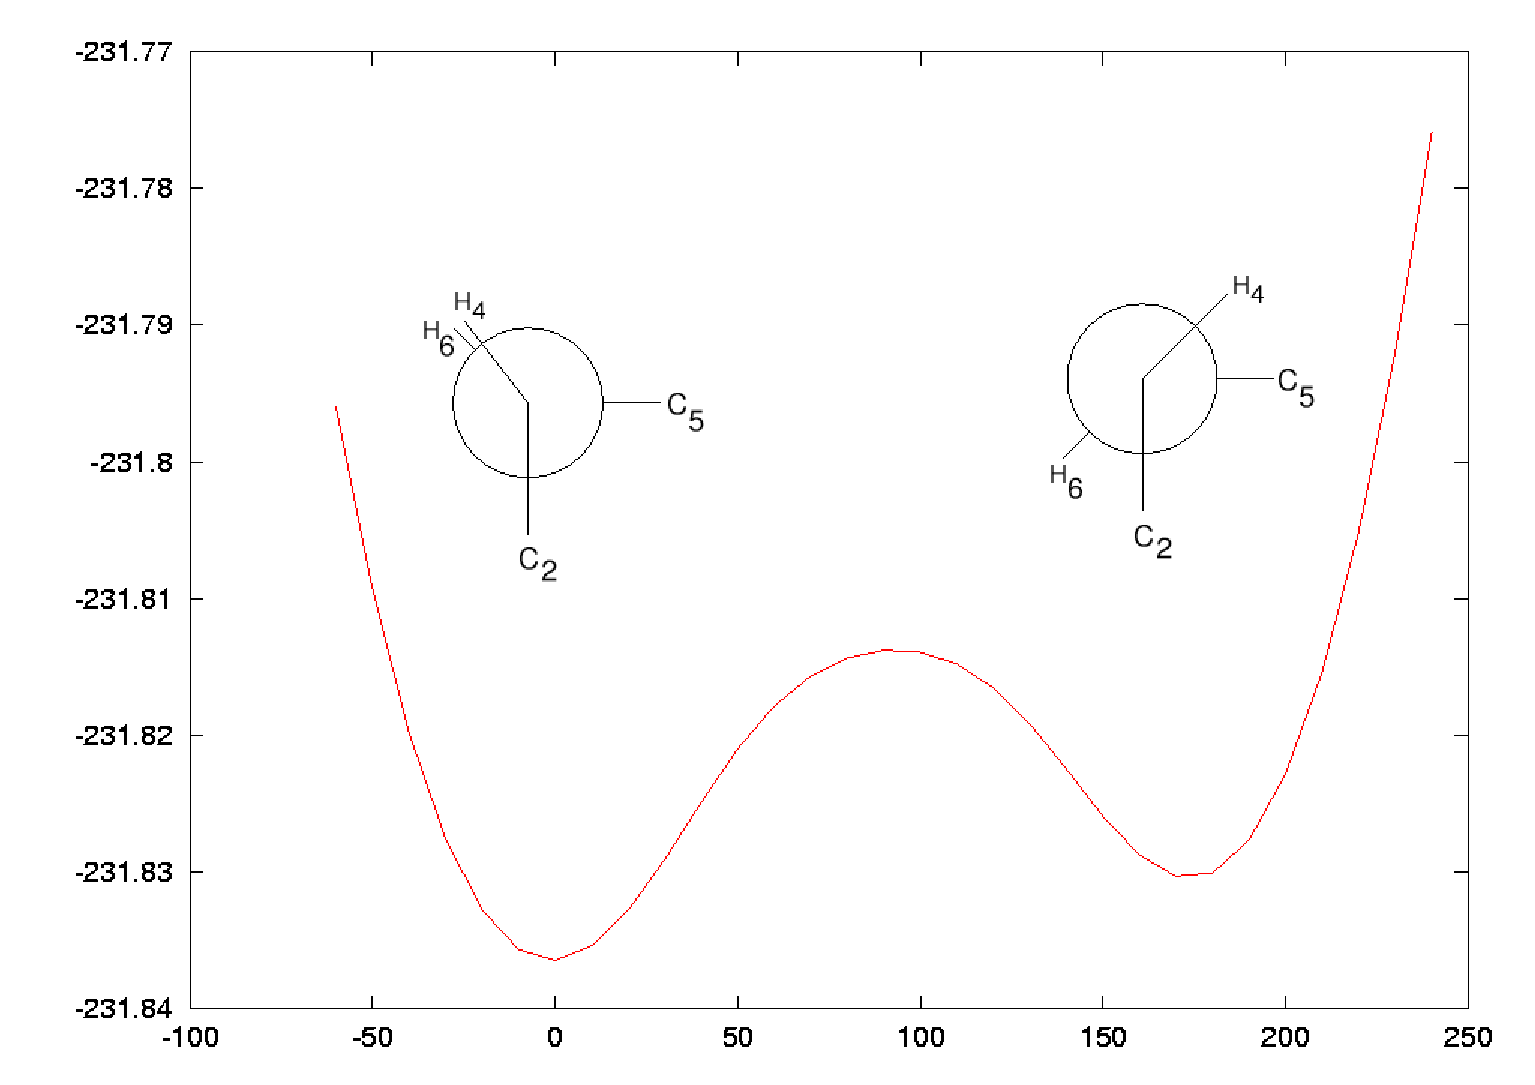
\includegraphics[width=10cm,keepaspectratio]{immagini/esatriene/c090.eps}
\end{center}
\end{figure}


Come \`e possibile notare, sono presenti due minimi, esattamente come nel
caso dell'etilene. Ciascun minimo rappresenta una possibile struttura di
equilibrio relativamente alla posizione degli idrogeni, una
approssimativamente sin-periplanare, l'altra approssimativamente
anti-periplanare. A differenza dell'etilene, tuttavia, \`e da notare che la
barriera di interconversione dalla sin alla anti \`e pi\`u bassa
(0.618 eV contro 1.45 eV per l'etilene). Questo \`e giustificabile
probabilmente in virt\`u della stabilizzazione dei due frammenti creati in
seguito alla rottura del doppio legame centrale. La formazione di due
frammenti vinilici contribuisce a ridurre l'energia della forma definita
dall'angolo diedro \mbox{H$_4$-C$_3$-C$_4$-H$_6$} a 90$^{\circ}$, in quanto tale forma
vede i frammenti privi di piramidalizzazione. Nel caso dell'etilene, si
ottenevano due orbitali $p$ completamente ortogonali che non potevano in
alcun modo interagire. Nel caso dell'esatriene e di tutti gli omologhi
superiori, ciascuno dei due orbitali \`e stabilizzato, e l'energia della
barriera risulta conseguentemente minore.

In queste condizioni, gli orbitali assumono combinazioni opportune: data la
simmetria C$_2$ della configurazione, si avranno combinazioni di simmetria
A o B sui gruppi di ciascun frammento.

Dal momento che ogni frammento pu\`o essere considerato un gruppo vinilico,
gli orbitali molecolari dello spazio attivo in questa situazione saranno 
definiti come in figura \ref{fig:esatriene_orbitali_c90_h90}
\pagebreak

\begin{figure}[htb]
\caption{\small Esatriene - spazio CAS per la configurazione con 
\mbox{H$_4$-C$_3$-C$_4$-H$_6$}=90$^{\circ}$ e
\mbox{C$_2$-C$_3$-C$_4$-C$_5$}=90$^{\circ}$ }
\label{fig:esatriene_orbitali_c90_h90}
\begin{center}
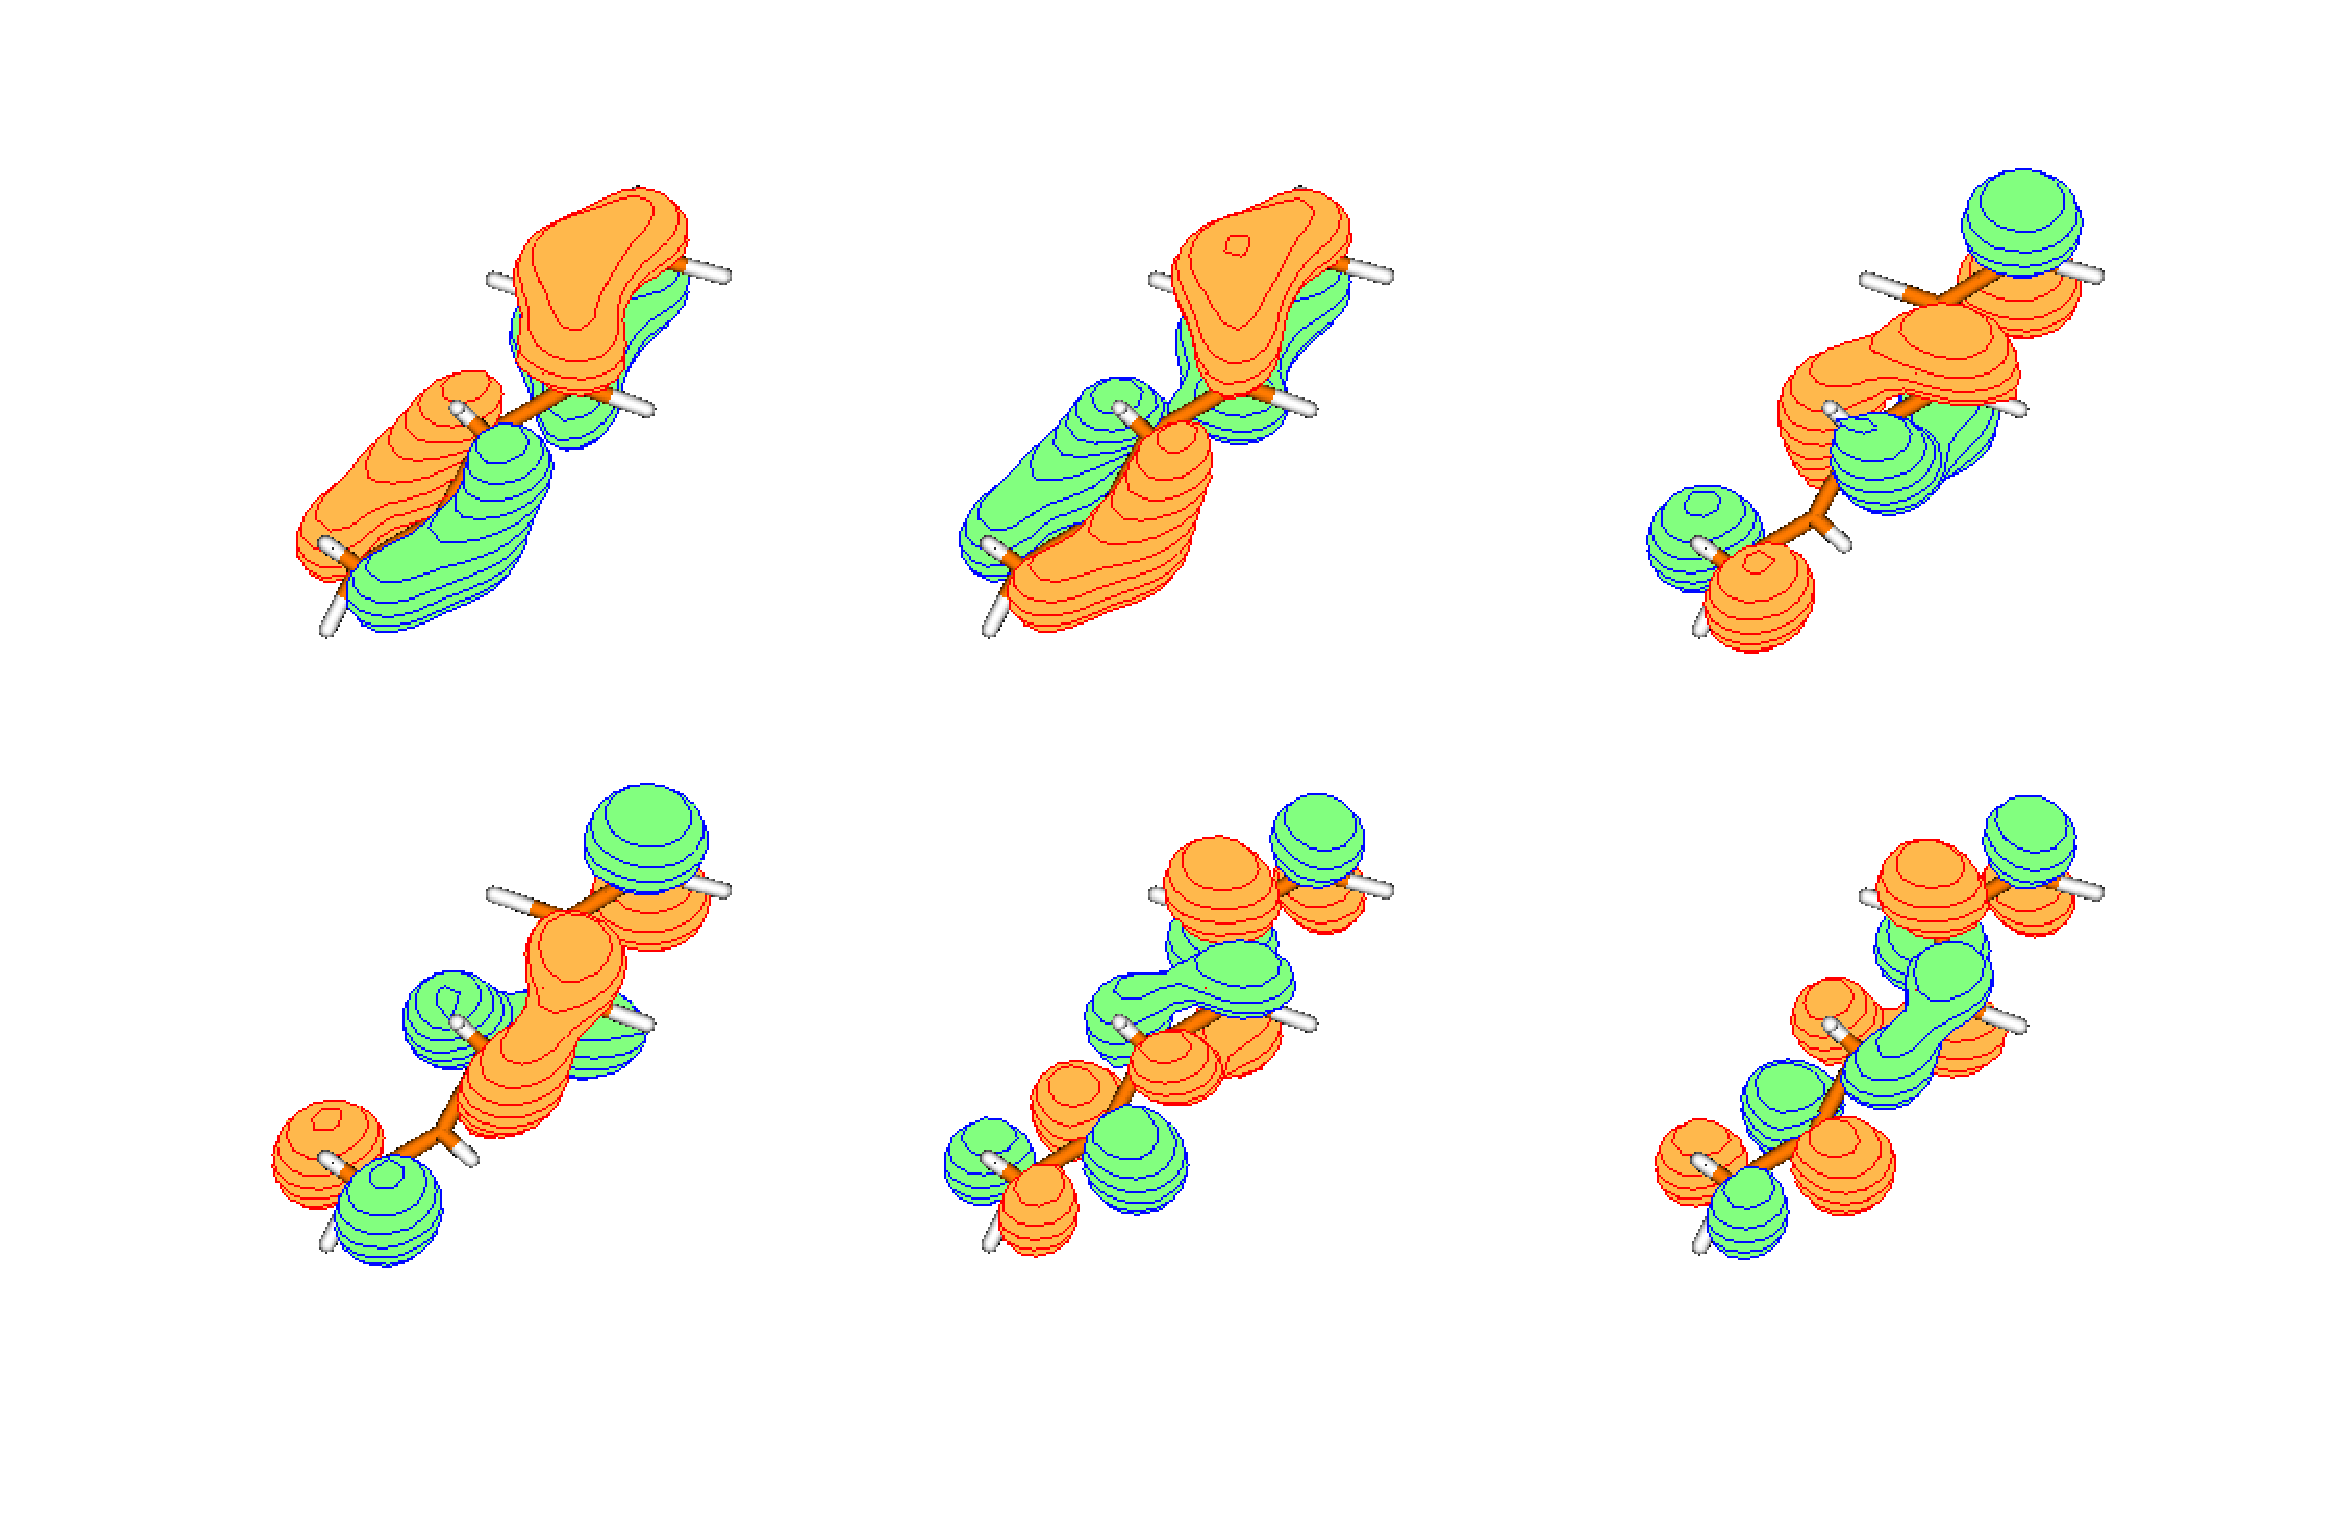
\includegraphics[width=12cm,keepaspectratio]{immagini/esatriene/orbitali_c90_h90.eps}
\end{center}
\end{figure}

Una volta ottenuto un set di orbitali per ogni posizione degli atomi di
idrogeno, si sono utilizzati come guess per ottenere le curve con angoli
diedri \mbox{C$_2$-C$_3$-C$_4$-C$_5$} inferiori e superiori di 90$^{\circ}$.

\begin{wrapfigure}{l}{8cm}
\includegraphics[angle=270,width=75mm,keepaspectratio]{immagini/esatriene/inviluppo.eps}
\caption{\small Esatriene - sezioni della superficie a vari angoli diedri C-C-C-C }
\label{fig:esatriene_inviluppo}
\end{wrapfigure}

Alcuni leggeri interventi si sono resi necessari nel caso che non si
ottenesse convergenza, tipicamente utilizzando il punto precedente o
successivo della curva. Alla fine si \`e ottenuta una superficie di
potenziale analoga a quella ottenuta per l'etilene ma, come gi\`a considerato
precedentemente, con una barriera a pi\`u bassa energia. 

\clearpage
\pagebreak

La superficie ottenuta si presta ad alcune considerazioni: \`e evidente che una
eventuale interconversione lungo questi gradi di libert\`a \`e difficilmente
realizzabile, sia perch\'e non vi \`e alcuna garanzia che questi gradi di
libert\`a siano gli unici in gioco nella interconversione, sia perch\'e questo
percorso prevede un forte spostamento di masse.

\begin{figure}[ht]
\begin{center}
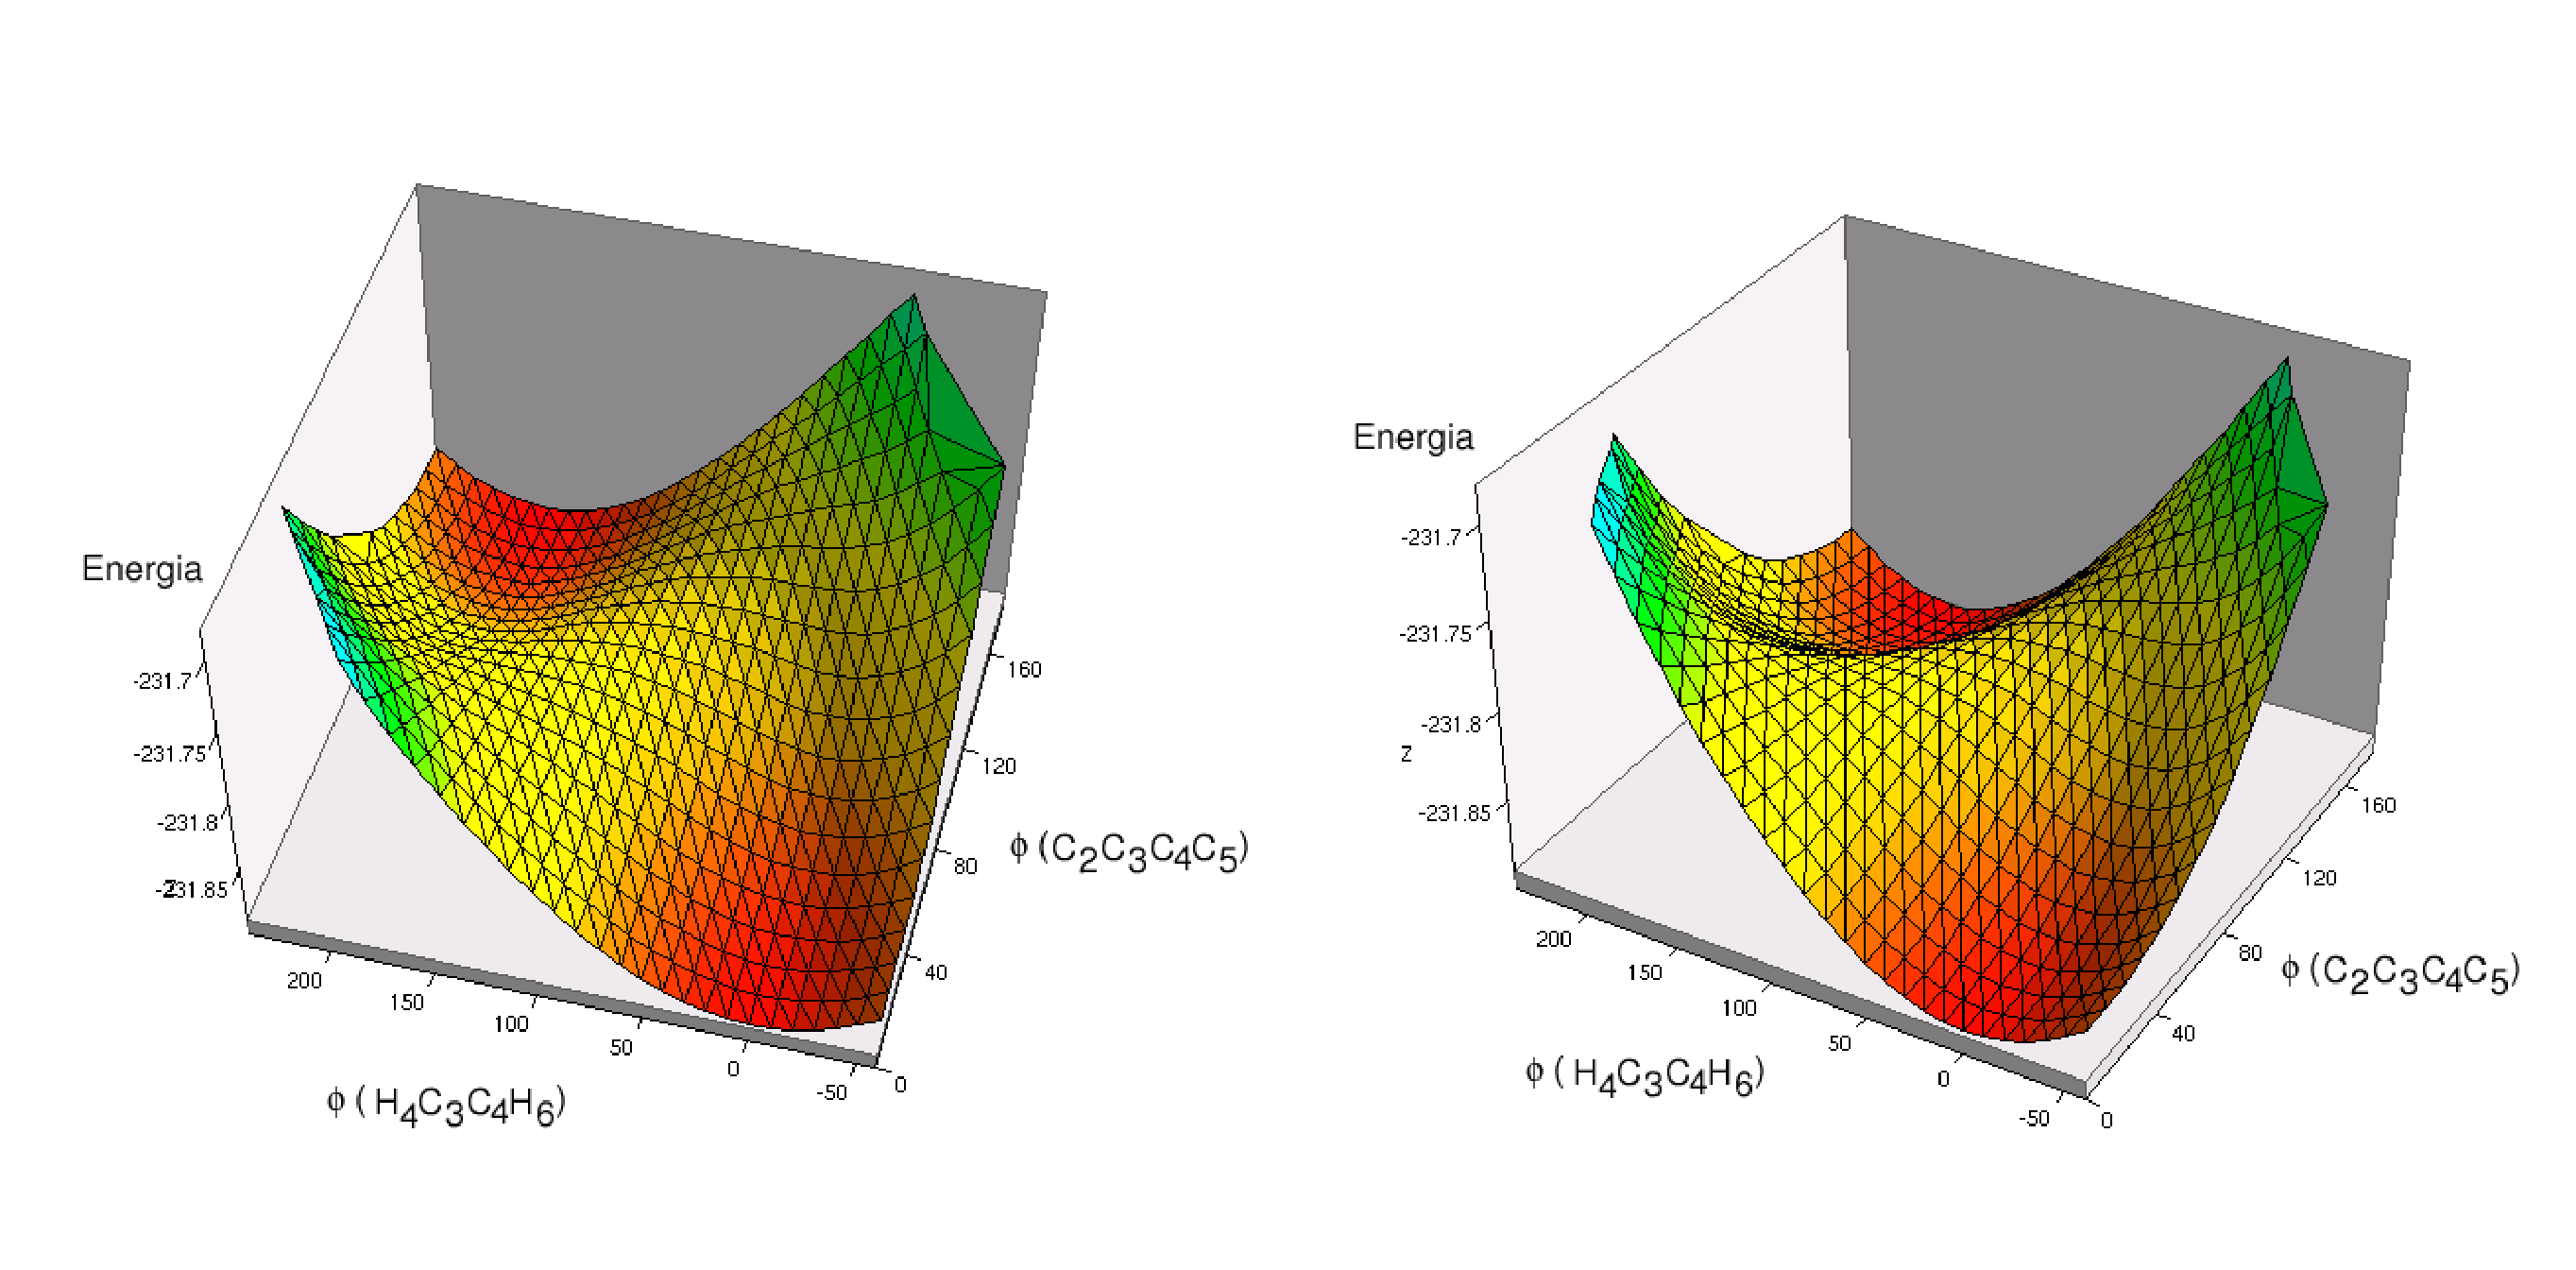
\includegraphics[angle=0,width=12cm,keepaspectratio]{immagini/esatriene/3d.eps}
\caption{\small Esatriene - superfici di potenziale}
\label{fig:esatriene_3d}
\end{center}
\end{figure}

Come conseguenza, difficilmente si tratta di una via di reale minimo energetico.
Nondimeno, una interconversione cis-trans che interessi esclusivamente lo stato
fondamentale deve necessariamente avvenire per via termica. Essendo i
polieni sistemi modello per molecole quali carotenoidi e acido retinoico,
precursori biologici di sistemi ad alta coniugazione responsabili di alcune
modalit\`a di pigmentazione e quali recettori luminosi, sar\`a centrale
nella loro interconversione il coinvolgimento di stati eccitati.
Tuttavia, \`e possibile evidenziare alcune caratteristiche interessanti:
\begin{itemize}
\item la forma sin periplanare correla, dal punto di vista strutturale, con
la forma cis del poliene. Al contrario la forma trans periplanare darebbe
origine ad un poliene i cui idrogeni centrali sono perpendicolari, e su
facce opposte, al piano molecolare, conformazione sicuramente non stabile,
come mostrato dalla ripidit\`a della curva a $\phi($C-C-C-C$) = 0^{\circ}$ e
$\phi($C-C-C-C$) = 180$.
\item analogamente, la forma trans-periplanare correla strutturalmente con
la forma trans del poliene. La forma cis-periplanare avrebbe sarebbe
analogamente non stabile, data la posizione degli idrogeni, ortogonali al
piano della molecola.
\item L'interconversione dalla forma cis ($\phi($C-C-C-C$) = 0^{\circ}$) alla forma
trans ($\phi($C-C-C-C$) = 180^{\circ}$) del poliene lungo i gradi di libert\`a definiti
impone un salto di una barriera energetica la cui altezza diminuisce via via
che l'angolo diedro $\phi($C-C-C-C$)$ aumenta. Questa barriera tende ad una
spalla che forza la risoluzione della specie verso la forma quasi
periplanare pi\`u stabile, in questo caso la trans. Analogo comportamento si
ottiene nell'interconversione dalla specie trans alla specie cis.
\end{itemize}

In virt\`u di quest'ultimo punto, il percorso di interconversione cis-trans
\`e differente dal percorso trans-cis. La molecola tende a seguire il minimo
locale della struttura che correla al meglio con lo stato di partenza, fino
a quando tale struttura non fornisce pi\`u uno stato di minimo energetico.
Quando ci\`o avviene, la struttura evolve verso lo stato di minimo energetico
modificando opportunamente la posizione degli idrogeni.

La figura \ref{fig:esatriene_mep_1} mostra i due differenti percorsi di
interconversione. Con la griglia di punti attuata per questa descrizione
(ogni 10 gradi del diedro tra i carboni)  \`e difficile localizzare dove
avvenga il rilassamento alla struttura geometricamente pi\`u stabile. Una
ulteriore difficolt\`a deriva dalla lentissima convergenza del calcolo di
ottimizzazione geometrica nelle vicinanze della spalla, punto nel quale il
gradiente \`e quasi nullo e, di conseguenza, l'eventuale riarrangiamento
verso il minimo assoluto procede molto lentamente.
La figura \ref{fig:esatriene_punti_minimo} fa riferimento alla posizione di
tali punti sul piano dei diedri.
\begin{figure}[ht]
\begin{center}
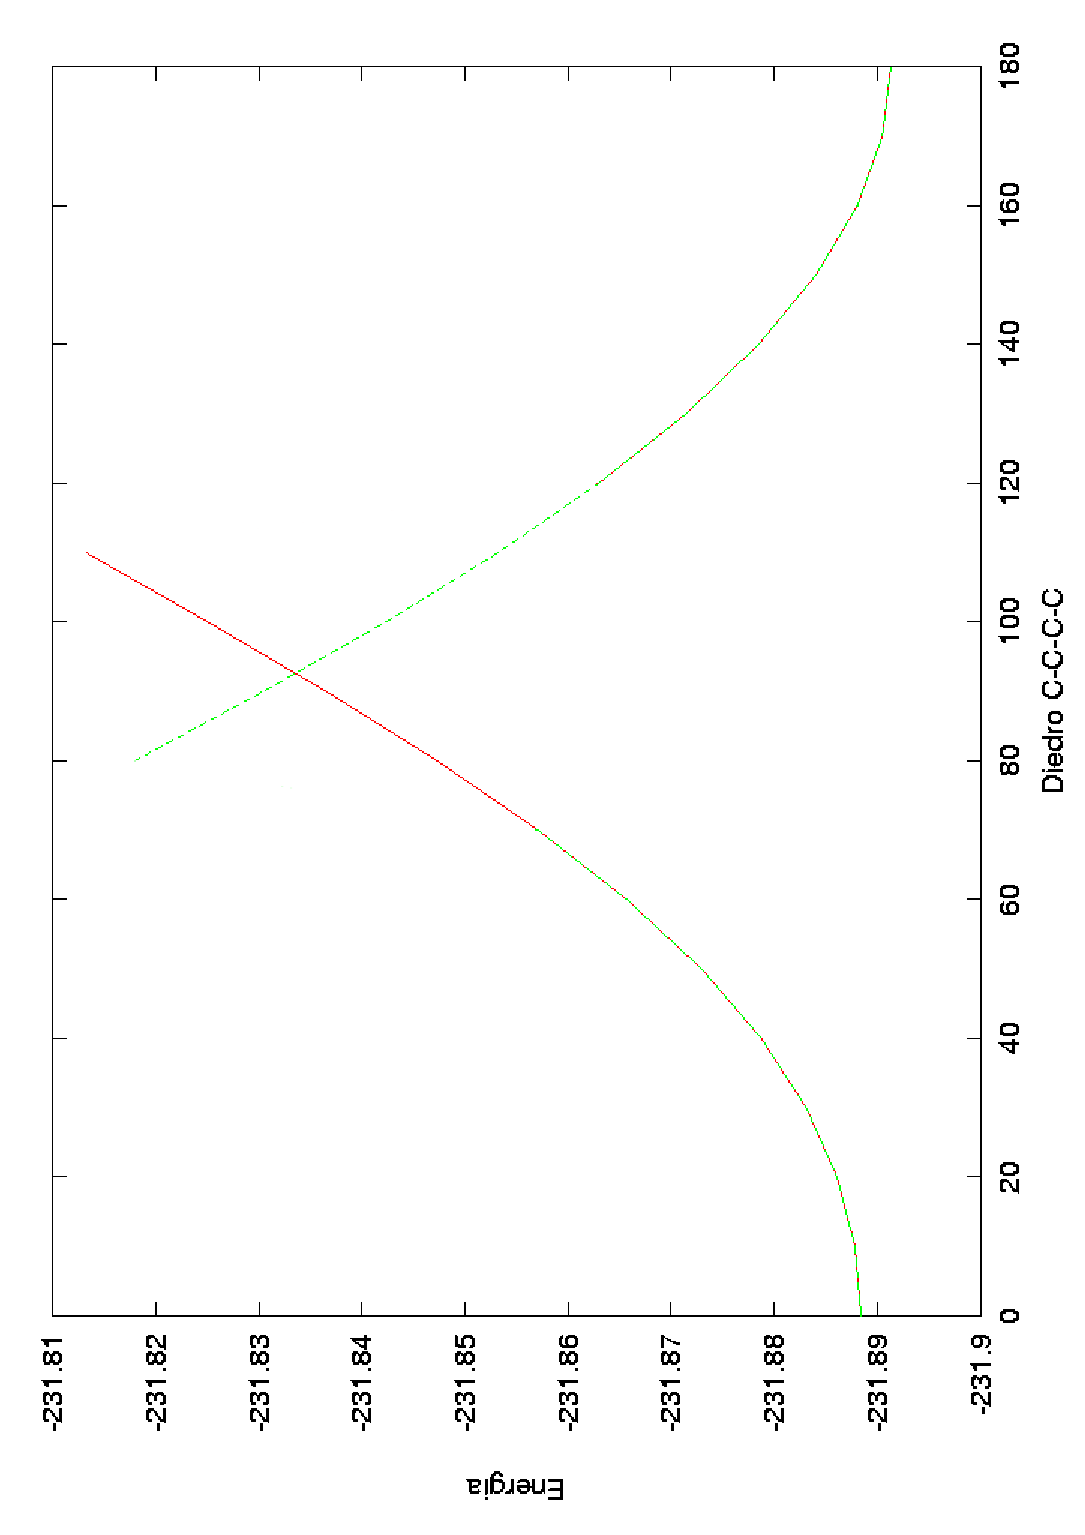
\includegraphics[angle=270,width=10cm,keepaspectratio]{immagini/esatriene/mep_1.eps}
\caption{\small Esatriene - percorso a minima energia lungo i gradi di
libert\`a definiti. Energie assolute}
\label{fig:esatriene_mep_1}
\end{center}
\end{figure}
\clearpage

\begin{figure}[ht]
\begin{center}
\includegraphics[angle=270,width=12cm,keepaspectratio]{immagini/esatriene/punti_minimo.eps}
\caption{\small Esatriene - percorso a minima energia lungo i gradi di
libert\`a definiti. Posizione sul piano definito dai diedri}
\label{fig:esatriene_punti_minimo}
\end{center}
\end{figure}

\`E quindi possibile approssimativamente definire tali punti di
interconversione in un intervallo compreso tra 70-80$^{\circ}$ per il mep
trans-cis e 110-120$^{\circ}$ per il mep cis-trans.

\subsubsection{Analisi perturbativa NEV-PT}

Successivamente allo studio approfondito a livello CASSCF, si \`e valutata
la variazione della struttura della superficie in seguito alla trattazione
perturbativa NEV-PT.

Sono state studiate le curve di potenziale rispetto al diedro H-C-C-H,
con angolo diedro C-C-C-C fissato a 0, 90 e 180$^{\circ}$. Tutte le
curve perturbative sono state traslate con opportuni valori al
fine di confrontarle dal punto di vista strutturale. Tali valori sono
di 0.710535 Hartree per le curve della trattazione strongly contracted e
0.710911 Hartree per le curve della partially contracted, valori che
rappresentano lo scarto tra le curve perturbative e la curva CASSCF nel 
punto con diedri C-C-C-C e H-C-C-H uguali a zero (ovvero la condizione di
equilibrio per l'isomero cis). 

L'analisi dell'andamento della perturbazione sulla curva a 0$^{\circ}$ ha
fornito il risultato in figura \ref{fig:esatriene_perturb_c0}.
Come si pu\`o notare, l'effetto perturbativo non introduce variazioni
nell'andamento della curva, ma si limita ad effettuare una traslazione
energetica dovuta al migliore contributo correlativo. In altri termini, il
contributo correlativo fornito dalla NEV-PT sulla funzione CASSCF \`e
uniforme per ogni punto della curva.

\begin{figure}[ht]
\begin{center}
\includegraphics[angle=270,width=12cm,keepaspectratio]{immagini/esatriene/perturb_c0.eps}
\caption{\small Esatriene - curva CASSCF (in rosso) con diedro C-C-C-C = 0$^{\circ}$, e curve perturbative
strongly (in verde) e partially (in blu), queste ultime traslate di 0.710535 e 0.710911 Hartree rispettivamente. Le
curve sono praticamente sovrapposte.}
\label{fig:esatriene_perturb_c0}
\end{center}
\end{figure}

Risultato molto simile si \`e ottenuto per la curva a 180$^{\circ}$, visibile
in figura \ref{fig:esatriene_perturb_c180}. In tale condizione \`e possibile
notare come il contributo perturbativo innalzi leggermente l'energia della
condizione pi\`u sfavorevole, ovvero quella per l'isomero trans con idrogeni
quasi ortogonali.

\begin{figure}[ht]
\begin{center}
\includegraphics[angle=270,width=12cm,keepaspectratio]{immagini/esatriene/perturb_c180.eps}
\caption{\small Esatriene - curva CASSCF (in rosso) con diedro C-C-C-C = 180$^{\circ}$, e curve perturbative
strongly (in verde) e partially (in blu), queste ultime traslate di 0.710535 e 0.710911 Hartree rispettivamente.}
\label{fig:esatriene_perturb_c180}
\end{center}
\end{figure}

Per quanto riguarda infine la curva con diedro C-C-C-C = 90$^{\circ}$,
incontriamo invece un certo cambiamento ad opera della trattazione
perturbativa: la barriera si innalza e si restringe, cos\`i come anche le due
buche di potenziale caratterizzanti i due stati coplanari per gli idrogeni. 

\begin{figure}[ht]
\begin{center}
\includegraphics[angle=270,width=12cm,keepaspectratio]{immagini/esatriene/perturb_c90.eps}
\caption{\small Esatriene - curva CASSCF (in rosso) con diedro C-C-C-C = 90$^{\circ}$, e curve perturbative
strongly (in verde) e partially (in blu), queste ultime traslate di 0.710535 e 0.710911 Hartree rispettivamente.}
\label{fig:esatriene_perturb_c90}
\end{center}
\end{figure}

\clearpage
\pagebreak

Il programma \texttt{dypc2} fornisce, nell'output, dettagli sul contributo
(come norma della correzione al primo ordine alla funzione d'onda e come energia)
sia per la correzione parzialmente contratta che
per quella fortemente contratta. Nelle figure \ref{fig:esatriene_norme_sc},
\ref{fig:esatriene_norme_pc}, \ref{fig:esatriene_energie_sc} e
\ref{fig:esatriene_energie_pc} sono mostrati rispettivamente gli andamenti,
rispetto al diedro H-C-C-H, dei valori delle norme strongly e partially e
delle correzioni alle energie strongly e partially, con diedro C-C-C-C
fissato a 90$^{\circ}$.

\`E possibile notare come il maggiore contributo alla correzione perturbativa
venga portato principalmente da $V(0)$ e $V(0')$, denotando chiaramente come 
le doppie eccitazioni siano fondamentali per la descrizione della molecola. %(Cfr. \cite{jcp-114-4-2001-1631} e \cite{jcp-112-2-2000-613})

\pagebreak
\begin{figure}[ht]
\begin{center}
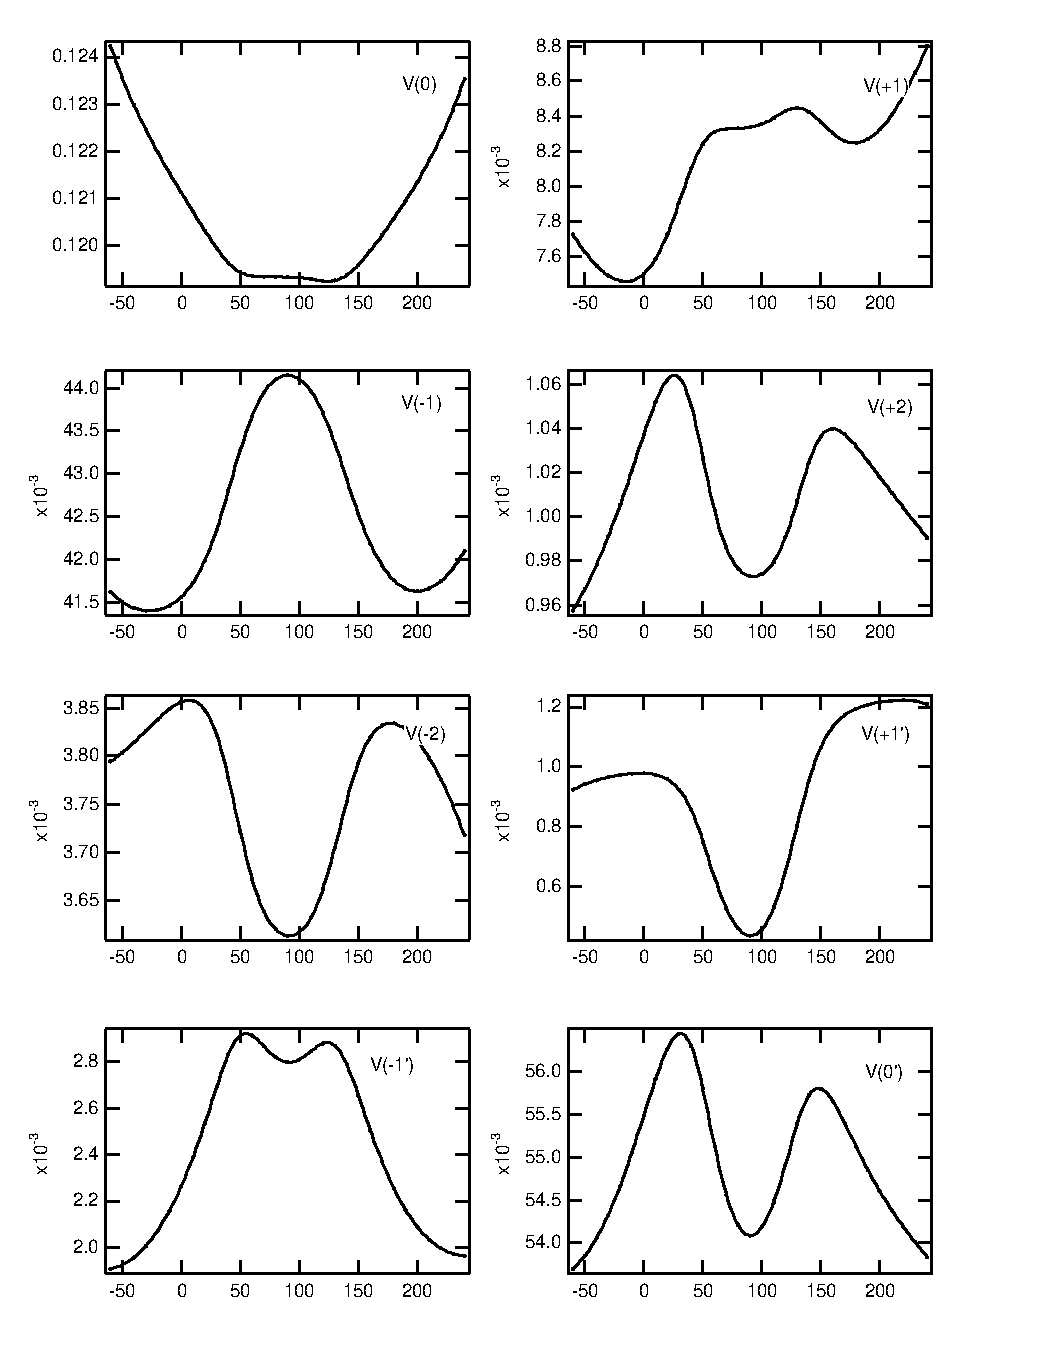
\includegraphics[angle=0,width=14cm,keepaspectratio]{immagini/esatriene/norme_sc.eps}
\caption{\small Esatriene - Norme per la correzione alla funzione d'onda.
Trattazione strongly contracted. }
\label{fig:esatriene_norme_sc}
\end{center}
\end{figure}
\pagebreak
\begin{figure}[ht]
\begin{center}
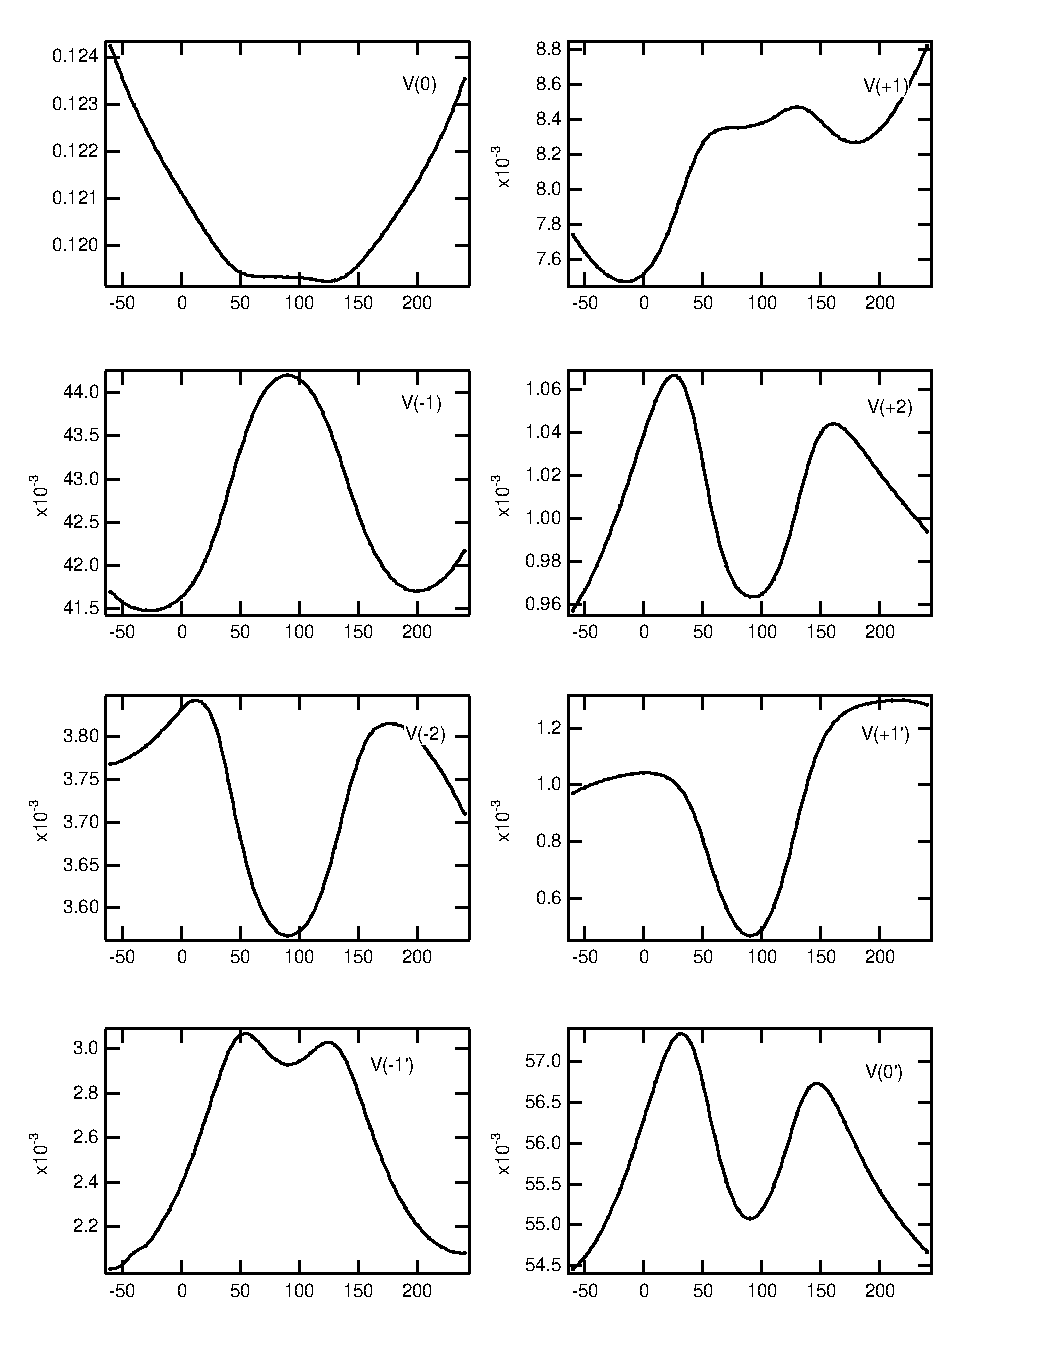
\includegraphics[angle=0,width=14cm,keepaspectratio]{immagini/esatriene/norme_pc.eps}
\caption{\small Esatriene - Norme per la correzione alla funzione d'onda.
Trattazione partially contracted. }
\label{fig:esatriene_norme_pc} 
\end{center}
\end{figure}
\pagebreak
\begin{figure}[ht]
\begin{center}
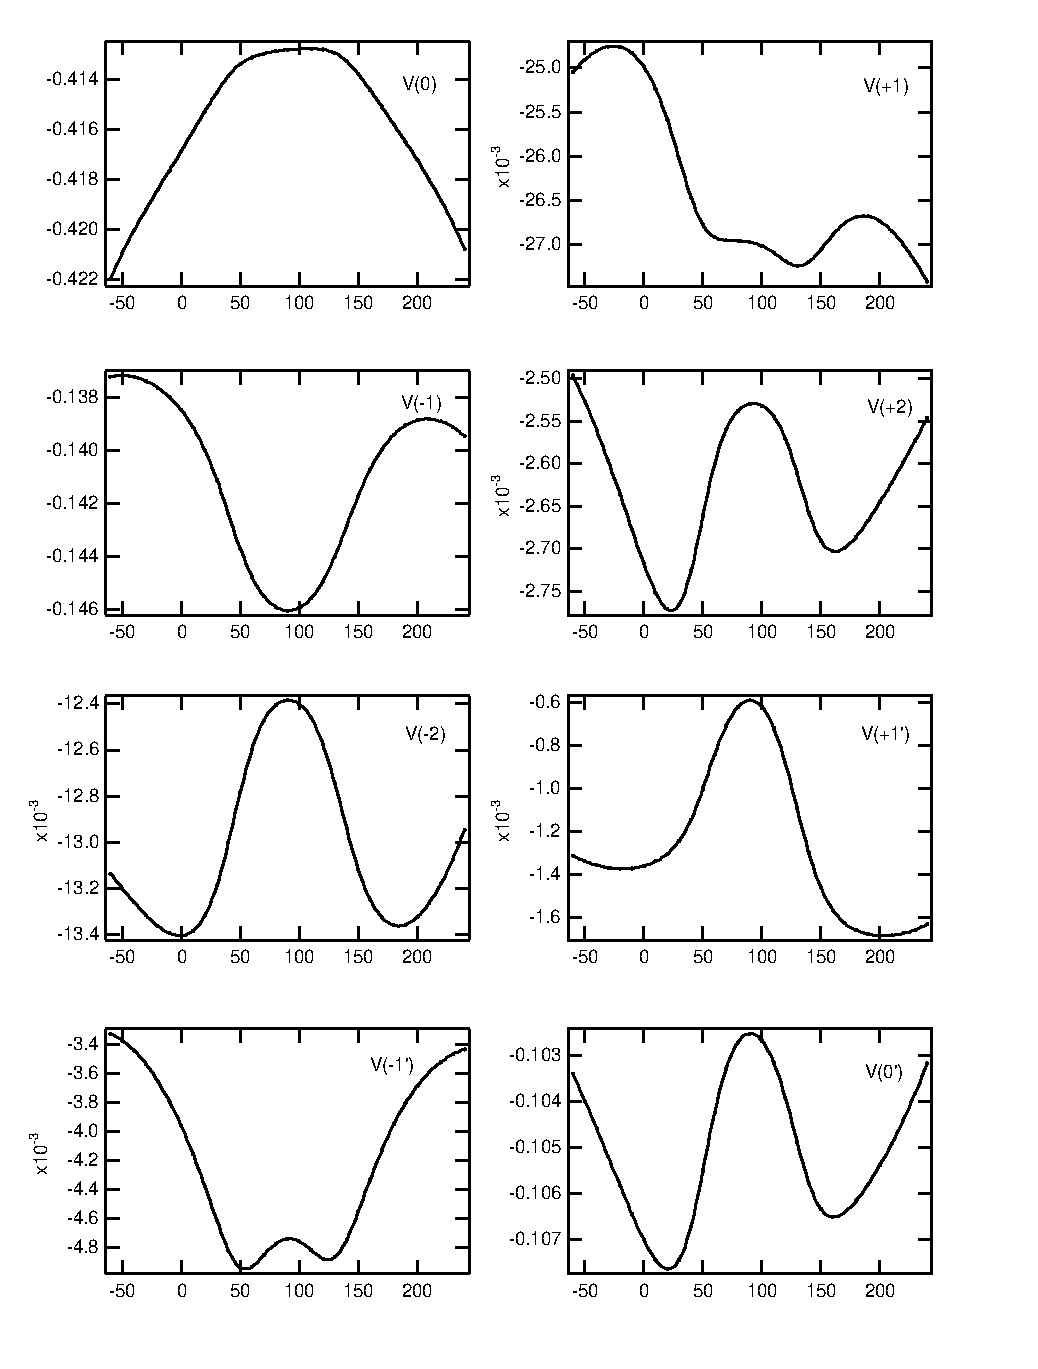
\includegraphics[angle=0,width=14cm,keepaspectratio]{immagini/esatriene/energie_sc.eps}
\caption{\small Esatriene - Contributi all'energia per l'applicazione
strongly contracted. Valori in Hartree. }
\label{fig:esatriene_energie_sc}
\end{center}
\end{figure}
\pagebreak
\begin{figure}[ht]
\begin{center}
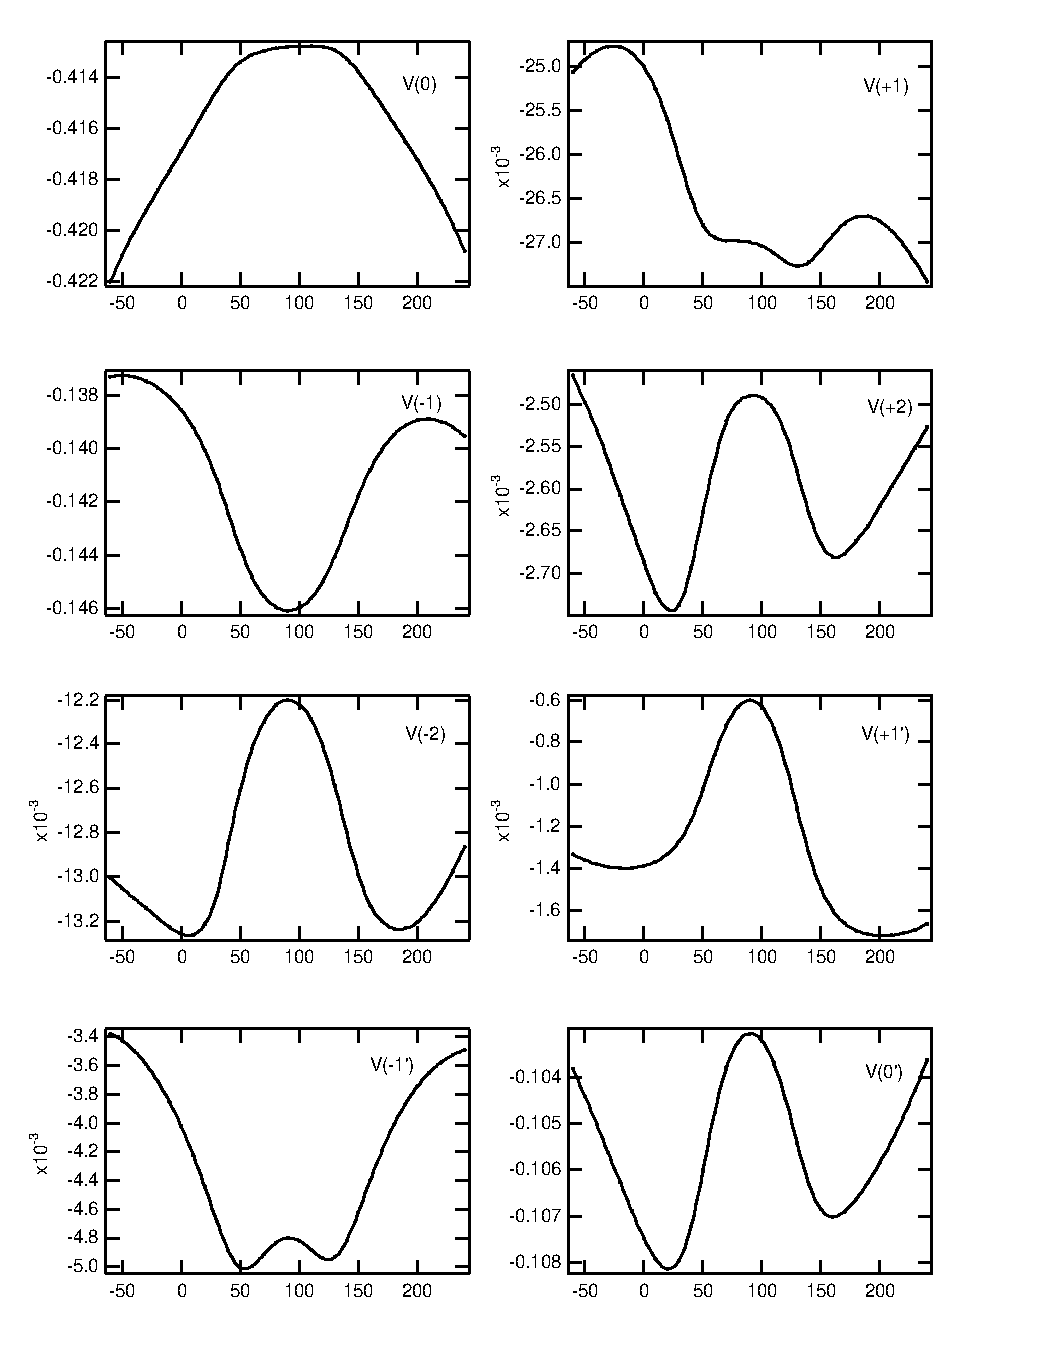
\includegraphics[angle=0,width=14cm,keepaspectratio]{immagini/esatriene/energie_pc.eps}
\caption{\small Esatriene - Contributi all'energia per l'applicazione
partially contracted. Valori in Hartree. }
\label{fig:esatriene_energie_pc}
\end{center}
\end{figure}
\pagebreak

\clearpage

\subsubsection{Energie di eccitazione verticale}

Sempre sulla molecola di esatriene si sono effettuati calcoli di valutazione
dell'energia di eccitazione verticale sia sull'isomero cis che sull'isomero
trans.

L'isomero cis, con simmetria $C_{2v}$, \`e stato ottimizzato con base 6-31G*
a livello CAS. Lo spazio attivo \`e costituito dai 6 elettroni
negli orbitali di natura $\pi$, orbitali appartenenti alle rappresentazioni
B$_1$ e A$_2$. La trattazione ha richiesto 92 configurazioni.
Al termine della procedura CASSCF, i numeri di occupazione per lo stato
fondamentale erano i seguenti
\begin{verbatim}
 Simmetria B1

   1.937856768   1.862253783   0.085298882

 Simmetria A2

   1.913147630   0.144502101   0.056940836
\end{verbatim}

Alla medesima geometria \`e stato condotto successivamente il calcolo per lo
stato eccitato 2A$_1$. I numeri di occupazione risultano essere
\begin{verbatim}
 Simmetria B1

   1.836468224   1.016224575   0.339483529

 Simmetria A2

   1.661825866   1.015253102   0.130744704
\end{verbatim}

\`E evidente la diversa distribuzione elettronica in questo stato eccitato.
A questo livello, l'energia di transizione risulta essere di 5.71 eV. Il
valore sperimentale \`e incerto, sebbene esistano alcuni riferimenti
(Cfr. \cite{jcp-114-4-2001-1631}) che forniscono un range da 4.57 a 5.04 eV.
Applicando la trattazione perturbativa, il risultato non cambia
notevolmente: l'approccio strongly contracted fornisce 5.69 eV, mentre il
partially contracted 5.67 eV. 

La medesima procedura \`e stata svolta per l'isomero trans, di simmetria
C$_{2h}$, relativamente allo stato eccitato 2$A_g$. Riferimenti esistenti
forniscono valori approssimativi, che spaziano in un range da
4.26 fino anche a 6.45 eV (vedere \cite{pccp-3-2001-2567}, \cite{jcp-112-2-2000-613},
\cite{jcp-92-1990-4622}). Il calcolo \`e stato condotto su base 6-31G* con
spazio CAS 6/6, ed il risultato ottenuto \`e 5.68 eV. A livello perturbativo,
il risultato resta sostanzialmente invariato: 5.68 eV su strongly contracted e
5.67 eV su partially.

Al fine di valutare meglio questa transizione, si \`e fatto uso di uno spazio
CAS espanso, ottenuto aggiungendo un orbitale virtuale per ogni simmetria.
In seguito a tale variazione, per descrivere il sistema sono ora necessarie
600 configurazioni per entrambi gli isomeri, contro le 92 dello spazio CAS
precedente.

La transizione per l'isomero cis fornisce, a livello CASSCF, 5.72 eV, e i
valori ricavati dalla trattazione perturbativa sono 5.74 e 5.72 eV, 
rispettivamente per strongly e partially.
L'isomero trans invece fornisce 5.69 eV, 5.73 e 5.70 rispettivamente per
CASSCF, strongly e partially.



\addcontentsline{toc}{chapter}{Conclusioni}
\pagebreak
\thispagestyle{empty}
{ \Large \textbf{Conclusioni} } 
\vspace{6mm} \\
In questo lavoro di tesi si sono eseguiti studi applicativi su sistemi di
varia natura, sfruttando la teoria perturbativa multireference NEV-PT. Gli
scopi prefissi sono stati raggiunti, ed in particolare si \`e dimostrata

\begin{itemize}
\item l'efficienza numerica della NEV-PT, che ottiene buoni risultati
mantenendo una buona scalabilit\`a, sia in termini di tempi macchina che in
termini di risorse hardware, questo grazie alla necessit\`a di effettuare
operazioni numeriche implicanti esclusivamente lo spazio attivo, di
dimensionalit\`a normalmente ridotta rispetto a quella della base orbitalica
totale.
\item la solidit\`a dell'algoritmo. In nessuno dei casi sottoposti ad
analisi si sono incontrate difficolt\`a computazionali come divergenze o
instabilit\`a.
\item l'applicabilit\`a dell'algoritmo perturbativo sia allo stato
fondamentale che agli stati eccitati. La descrizione di tali stati comporta
errori simili, in modo tale da rendere accettabile il risultato finale per
l'energia di transizione.
\item l'utilizzo di un approccio strongly contracted fornisce valori di poco
differenti da un'analoga trattazione partially contracted, con un costo
computazionale alquanto minore.
\item la risoluzione di molti problemi di tipo formale, 
quali la separabilit\`a stretta (size consistence) e l'assenza di stati
intrusi.
\end{itemize}


\addcontentsline{toc}{chapter}{Bibliografia}
\nocite{*}
\bibliographystyle{acs}
\bibliography{tesi}

\end{document}
